\documentclass[edeposit,fullpage,11pt]{uiucthesis2009}
% Use draftthesis for notes and date markings on every page.  Useful when you
%   have multiple copies floating around.
% Use offcenter for the extra .5 inch on the left side. Needed with fullpage and fancy.
% Use mixcasechap for compatibility with hyperref package, which does NOT like all caps default
% Use edeposit for the adviser/committee on the title page.
% Use tocnosub to suppress subsection and lower entries in the TOC.
% PhD candidates use "proquest" for the proquest abstract.

\makeatletter

\usepackage{setspace}
%\usepackage{epsfig}  % for figures
\usepackage{graphicx}  % another package that works for figures
\usepackage{multirow}
\usepackage{placeins}
\usepackage{caption}  % allows center figures caption
\usepackage{booktabs} % nice rules (thick lines) for tables
\usepackage{array}
\usepackage{tabularx}
\usepackage[table]{xcolor}
\newcolumntype{b}{>{\hsize=1.0\hsize}X}
\newcolumntype{s}{>{\hsize=.5\hsize}X}
\newcolumntype{m}{>{\hsize=.75\hsize}X}
\newcolumntype{x}{>{\hsize=.25\hsize}X}
\newcolumntype{L}{>{\raggedright\arraybackslash}X}
\newcolumntype{R}{>{\raggedleft\arraybackslash}X} 
\def\arraystretch{1}
\graphicspath{{figures/}}
%\usepackage{subfigure}  % for subfigures
\usepackage{amsmath}  % for math spacing
%\usepackage{amssymb}  % for math spacing
%\usepackage{url}  % Hyphenation of URLs.
\usepackage{lscape}  % Useful for wide tables or figures.
\usepackage[justification=raggedright]{caption}	% makes captions ragged right - thanks to Bryce Lobdell
%\usepackage[font=small,labelfont=bf]{caption}
\usepackage[acronym,toc]{glossaries}  % acronyms inclusion
\usepackage{color,soul}
\makeglossary
\usepackage{xspace}
\usepackage{float}
\usepackage{subcaption}
\newcommand{\Cyclus}{\textsc{Cyclus}\xspace}%
\newcommand{\Cycamore}{\textsc{Cycamore}\xspace}%
\newcommand{\deploy}{\texttt{d3ploy}\xspace}%
\glspatchtabularx

\usepackage{amsmath}%
\usepackage{MnSymbol}%
\usepackage{wasysym}%
\usepackage{adjustbox}
\usepackage{hyperref}
\usepackage{enumitem}

\usepackage{tikz}
\usetikzlibrary{positioning, arrows, decorations, shapes}
\usetikzlibrary{shapes.geometric,arrows}
\def\checkmark{\tikz\fill[scale=0.4](0,.35) -- (.25,0) -- (1,.7) -- (.25,.15) -- cycle;} 

\definecolor{illiniblue}{HTML}{B1C6E2}
\definecolor{illiniorange}{HTML}{f8c2a2}
\definecolor{pink}{HTML}{e2b1c2}
\definecolor{green}{HTML}{c2e2b1}
\definecolor{purple}{HTML}{b9b1e2}
\tikzstyle{snoblock} = [rectangle, 
text width=5em, text centered,  minimum height=0em]
\tikzstyle{noblock} = [rectangle, 
text width=5em, text centered,  minimum height=3em]
\tikzstyle{loblock} = [rectangle, draw, fill=illiniorange, 
text width=15em, text centered, rounded corners, minimum height=3em]
\tikzstyle{lbblock} = [rectangle, draw, fill=illiniblue, 
text width=15em, text centered, rounded corners, minimum height=3em]
\tikzstyle{oblock} = [rectangle, draw, fill=illiniorange, 
text width=10em, text centered, rounded corners, minimum height=3em]
\tikzstyle{bblock} = [rectangle, draw, fill=illiniblue, 
text width=10em, text centered, rounded corners, minimum height=3em]
\tikzstyle{arrow} = [thick,->,>=stealth]
\tikzstyle{pblock} = [rectangle, draw, fill=pink, 
text width=10em, text centered, rounded corners, minimum height=3em]
\tikzstyle{gblock} = [rectangle, draw, fill=green, 
text width=10em, text centered, rounded corners, minimum height=3em]
\tikzstyle{ppblock} = [rectangle, draw, fill=purple, 
text width=10em, text centered, rounded corners, minimum height=3em]
\tikzstyle{lppblock} = [rectangle, draw, fill=purple, 
text width=15em, text centered, rounded corners, minimum height=3em]
\tikzstyle{arrow} = [thick,->,>=stealth]
\tikzstyle{bbblock} = [rectangle, draw, fill=illiniblue, 
text width=1em, text centered, rounded corners, minimum height=1em]
\tikzstyle{boblock} = [rectangle, draw, fill=illiniorange, 
text width=1em, text centered, rounded corners, minimum height=1em]
\tikzstyle{bpblock} = [rectangle, draw, fill=pink, 
text width=1em, text centered, rounded corners, minimum height=1em]
\tikzstyle{bgblock} = [rectangle, draw, fill=green, 
text width=1em, text centered, rounded corners, minimum height=1em]
\tikzstyle{bppblock} = [rectangle, draw, fill=purple, 
text width=1em, text centered, rounded corners, minimum height=1em]
\usepackage[document]{ragged2e}
% Uncomment the appropriate one of the following four lines:
%\msthesis
\phdthesis
%\otherdoctorate[abbrev]{Title of Degree}
%\othermasters[abbrev]{Title of Degree}

\title{Generative Reactor Design}
\author{Gwendolyn J.Y. Chee}
\department{Nuclear, Plasma, and Radiological Engineering}
\degreeyear{2021}

% Advisor name is required for
% - doctoral students for the ProQuest abstract
% - master's students who do not have a master's committee
%\advisor{Professor Kathryn D. Huff}

% Uncomment the \committee command for
% - all doctoral students
% - master's students who have a master's committee
\committee{Assistant Professor Kathryn D. Huff, Advisor \\
           Associate Professor Tomasz Kozlowski \\
           Professor James F. Stubbins} 

\begin{document}
%\newacronym{<++>}{<++>}{<++>}
\newacronym[longplural={metric tons of heavy metal}]{MTHM}{MTHM}{metric ton of heavy metal}
\newacronym{3D CAD}{3D CAD}{three-dimensional Computer-Aided Design}
\newacronym{ABM}{ABM}{agent-based modeling}
\newacronym{ACDIS}{ACDIS}{Program in Arms Control \& Domestic and International Security}
\newacronym{AHTR}{AHTR}{Advanced High Temperature Reactor}
\newacronym{AI}{AI}{Artificial Intelligence}
\newacronym{AM}{AM}{Additive Manufacturing}
\newacronym{AMAFT}{AMAFT}{Additive Manufacturing as an Alternative Fabrication Technique}
\newacronym{ANDRA}{ANDRA}{Agence Nationale pour la gestion des D\'echets RAdioactifs, the French National Agency for Radioactive Waste Management}
\newacronym{ANL}{ANL}{Argonne National Laboratory}
\newacronym{ANS}{ANS}{American Nuclear Society}
\newacronym{API}{API}{application programming interface}
\newacronym{ARE}{ARE}{Aircraft Reactor Experiment}
\newacronym{ARFC}{ARFC}{Advanced Reactors and Fuel Cycles}
\newacronym{ARMA}{ARMA}{Autoregressive Moving Average}
\newacronym{ARCH}{ARCH}{Autoregressive Heteroskedasticity}
\newacronym{ARIMA}{ARIMA}{Auto-Regressive Integrated Moving Averages}
\newacronym{ASME}{ASME}{American Society of Mechanical Engineers}
\newacronym{ATWS}{ATWS}{Anticipated Transient Without Scram}
\newacronym{BDBE}{BDBE}{Beyond Design Basis Event}
\newacronym{BIDS}{BIDS}{Berkeley Institute for Data Science}
\newacronym{BNL}{BNL}{Brookhaven National Laboratory}
\newacronym{CAFCA}{CAFCA}{ Code for Advanced Fuel Cycles Assessment }
\newacronym{CDTN}{CDTN}{Centro de Desenvolvimento da Tecnologia Nuclear}
\newacronym{CFD}{CFD}{Computational Fluid Dynamics}
\newacronym{CEA}{CEA}{Commissariat \`a l'\'Energie Atomique et aux \'Energies Alternatives}
\newacronym{CI}{CI}{continuous integration}
\newacronym{CIEMAT}{CIEMAT}{Centro de Investigaciones Energéticas, Medioambientales y Tecnológicas}
\newacronym{CNEN}{CNEN}{Comiss\~{a}o Nacional de Energia Nuclear}
\newacronym{CNERG}{CNERG}{Computational Nuclear Engineering Research Group}
\newacronym{CNRS}{CNRS}{Le Centre National De La Recherche Scientifique}
\newacronym{COSI}{COSI}{Commelini-Sicard}
\newacronym{COTS}{COTS}{commercial, off-the-shelf}
\newacronym{CSNF}{CSNF}{commercial spent nuclear fuel}
\newacronym{CTAH}{CTAHs}{Coiled Tube Air Heaters}
\newacronym{CUBIT}{CUBIT}{CUBIT Geometry and Mesh Generation Toolkit}
\newacronym{CURIE}{CURIE}{Centralized Used Fuel Resource for Information Exchange}
\newacronym{DAG}{DAG}{directed acyclic graph}
\newacronym{DANESS}{DANESS}{Dynamic Analysis of Nuclear Energy System Strategies}
\newacronym{DBE}{DBE}{Design Basis Event}
\newacronym{DEAP}{DEAP}{Distributed Evolutionary Algorithms in Python}
\newacronym{DESAE}{DESAE}{Dynamic Analysis of Nuclear Energy Systems Strategies}
\newacronym{DHS}{DHS}{Department of Homeland Security}
\newacronym{DNBR}{DNBR}{Departure from nucleate boiling ratio}
\newacronym{DOE}{DOE}{Department of Energy}
\newacronym{dpa}{dpa}{displacements per atom}
\newacronym{DRACS}{DRACS}{Direct Reactor Auxiliary Cooling System}
\newacronym{DRE}{DRE}{dynamic resource exchange}
\newacronym{DSNF}{DSNF}{DOE spent nuclear fuel}
\newacronym{DYMOND}{DYMOND}{Dynamic Model of Nuclear Development }
\newacronym{EBM}{EBM}{electron beam melting}
\newacronym{EBS}{EBS}{Engineered Barrier System}
\newacronym{EDF}{EDF}{Électricité de France}
\newacronym{EDZ}{EDZ}{Excavation Disturbed Zone}
\newacronym{EG}{EG}{Evaluation Group}
\newacronym{EIA}{EIA}{U.S. Energy Information Administration}
\newacronym{EPA}{EPA}{Environmental Protection Agency}
\newacronym{EPR}{EPR}{European Pressurized Reactors}
\newacronym{EP}{EP}{Engineering Physics}
\newacronym{EU}{EU}{European Union}
\newacronym{FCM}{FCM}{fully ceramic microencapsulated}
\newacronym{FCO}{FCO}{Fuel Cycle Options}
\newacronym{FCT}{FCT}{Fuel Cycle Technology}
\newacronym{FEHM}{FEHM}{Finite Element Heat and Mass Transfer}
\newacronym{FEPs}{FEPs}{Features, Events, and Processes}
\newacronym{FHR}{FHR}{Fluoride-Salt-Cooled High-Temperature Reactor}
\newacronym{FLiBe}{FLiBe}{Fluoride-Lithium-Beryllium}
\newacronym{FM}{FM}{ferritic/martensitic}
\newacronym{FP}{FP}{Fission Product}
\newacronym{GA}{GA}{Genetic Algorithm}
\newacronym{GDSE}{GDSE}{Generic Disposal System Environment}
\newacronym{GDSM}{GDSM}{Generic Disposal System Model}
\newacronym{GENIUSv1}{GENIUSv1}{Global Evaluation of Nuclear Infrastructure Utilization Scenarios, Version 1}
\newacronym{GENIUSv2}{GENIUSv2}{Global Evaluation of Nuclear Infrastructure Utilization Scenarios, Version 2}
\newacronym{GENIUS}{GENIUS}{Global Evaluation of Nuclear Infrastructure Utilization Scenarios}
\newacronym{GFR}{GFR}{Gas-Cooled Fast Reactor System}
\newacronym{GHG}{GHG}{Greenhouse Gas}
\newacronym{GPAM}{GPAM}{Generic Performance Assessment Model}
\newacronym{GRSAC}{GRSAC}{Graphite Reactor Severe Accident Code}
\newacronym{GUI}{GUI}{graphical user interface}
\newacronym{HFIR}{HFIR}{High Flux Isotope Reactor}
\newacronym{HLW}{HLW}{high level waste}
\newacronym{HPC}{HPC}{high-performance computing}
\newacronym{HTC}{HTC}{high-throughput computing}
\newacronym{HTGR}{HTGR}{High Temperature Gas-Cooled Reactor}
\newacronym{IAEA}{IAEA}{International Atomic Energy Agency}
\newacronym{IEMA}{IEMA}{Illinois Emergency Mangament Agency}
\newacronym{IHLRWM}{IHLRWM}{International High Level Radioactive Waste Management}
\newacronym{INL}{INL}{Idaho National Laboratory}
\newacronym{IPRR1}{IRP-R1}{Instituto de Pesquisas Radioativas Reator 1}
\newacronym{IRP}{IRP}{Integrated Research Project}
\newacronym{IRSN}{IRSN}{Institute for Radiological Protection and Nuclear Safety}
\newacronym{ISFSI}{ISFSI}{Independent Spent Fuel Storage Installation}
\newacronym{ISRG}{ISRG}{Independent Student Research Group}
\newacronym{JAEA}{JAEA}{Japanese Atomic Energy Agency}
\newacronym{JFNK}{JFNK}{Jacobian-Free Newton Krylov}
\newacronym{LANL}{LANL}{Los Alamos National Laboratory}
\newacronym{LBNL}{LBNL}{Lawrence Berkeley National Laboratory}
\newacronym{LCOE}{LCOE}{levelized cost of electricity}
\newacronym{L-DED}{L-DED}{laser directed energy deposition}
\newacronym{LDRD}{LDRD}{laboratory directed research and development}
\newacronym{LEU}{LEU}{low-enriched uranium}
\newacronym{LFR}{LFR}{Lead-Cooled Fast Reactor}
\newacronym{LLNL}{LLNL}{Lawrence Livermore National Laboratory}
\newacronym{LMFBR}{LMFBR}{Liquid Metal Fast Breeder Reactor}
\newacronym{LOFC}{LOFC}{Loss of Forced Cooling}
\newacronym{LOHS}{LOHS}{Loss of Heat Sink}
\newacronym{LOLA}{LOLA}{Loss of Large Area}
\newacronym{LP}{LP}{linear program}
\newacronym{LPD}{LPD}{Local power density}
\newacronym{LWR}{LWR}{Light Water Reactor}
\newacronym{MAGNOX}{MAGNOX}{Magnesium Alloy Graphie Moderated Gas Cooled Uranium Oxide Reactor}
\newacronym{MA}{MA}{minor actinide}
\newacronym{MCNP}{MCNP}{Monte Carlo N-Particle code}
\newacronym{MILP}{MILP}{mixed-integer linear program}
\newacronym{MIT}{MIT}{Massachusetts Institute of Technology}
\newacronym{MOAB}{MOAB}{Mesh-Oriented datABase}
\newacronym{MOOSE}{MOOSE}{Multiphysics Object-Oriented Simulation Environment}
\newacronym{MOSART}{MOSART}{Molten Salt Actinide Recycler and Transmuter}
\newacronym{MOX}{MOX}{mixed oxide}
\newacronym{MPI}{MPI}{Message Passing Interface}
\newacronym{MSBR}{MSBR}{Molten Salt Breeder Reactor}
\newacronym{MSFR}{MSFR}{Molten Salt Fast Reactor}
\newacronym{MSRE}{MSRE}{Molten Salt Reactor Experiment}
\newacronym{MSR}{MSR}{Molten Salt Reactor}
\newacronym{NAGRA}{NAGRA}{National Cooperative for the Disposal of Radioactive Waste}
\newacronym{NEA}{NEA}{Nuclear Energy Agency}
\newacronym{NEAMS}{NEAMS}{Nuclear Engineering Advanced Modeling and Simulation}
\newacronym{NEUP}{NEUP}{Nuclear Energy University Programs}
\newacronym{NFC}{NFC}{Nuclear Fuel Cycle}
\newacronym{NFCSim}{NFCSim}{Nuclear Fuel Cycle Simulator}
\newacronym{NGNP}{NGNP}{Next Generation Nuclear Plant}
\newacronym{NMR-50}{NMR-50}{Purdue Novel Modular Reactor}
\newacronym{NMWPC}{NMWPC}{Nuclear MW Per Capita}
\newacronym{NNL}{NNL}{National Nuclear Laboratory}
\newacronym{NNSA}{NNSA}{National Nuclear Security Administration}
\newacronym{NPP}{NPP}{Nuclear Power Plant}
\newacronym{NPRE}{NPRE}{Department of Nuclear, Plasma, and Radiological Engineering}
\newacronym{NQA1}{NQA-1}{Nuclear Quality Assurance - 1}
\newacronym{NRC}{NRC}{Nuclear Regulatory Commission}
\newacronym{NSF}{NSF}{National Science Foundation}
\newacronym{NSSC}{NSSC}{Nuclear Science and Security Consortium}
\newacronym{NUWASTE}{NUWASTE}{Nuclear Waste Assessment System for Technical Evaluation}
\newacronym{NWF}{NWF}{Nuclear Waste Fund}
\newacronym{NWTRB}{NWTRB}{Nuclear Waste Technical Review Board}
\newacronym{OCRWM}{OCRWM}{Office of Civilian Radioactive Waste Management}
\newacronym{OECD}{OECD}{Organisation for Economic Co-operation and Development}
\newacronym{ORION}{ORION}{ORION}
\newacronym{ORNL}{ORNL}{Oak Ridge National Laboratory}
\newacronym{PARCS}{PARCS}{Purdue Advanced Reactor Core Simulator}
\newacronym{PCA}{PCA}{Particle Collision Algorithm}
\newacronym{PBAHTR}{PB-AHTR}{Pebble Bed Advanced High Temperature Reactor}
\newacronym{PBFHR}{PB-FHR}{Pebble-Bed Fluoride-Salt-Cooled High-Temperature Reactor}
\newacronym{PEI}{PEI}{Peak Environmental Impact}
\newacronym{PH}{PRONGHORN}{PRONGHORN}
\newacronym{PIRT}{PIRT}{Phenomena Identification and Ranking Table}
\newacronym{PPF}{PPF}{Power peaking factor}
\newacronym{PRIS}{PRIS}{Power Reactor Information System}
\newacronym{PRKE}{PRKE}{Point Reactor Kinetics Equations}
\newacronym{PSPG}{PSPG}{Pressure-Stabilizing/Petrov-Galerkin}
\newacronym{PWAR}{PWAR}{Pratt and Whitney Aircraft Reactor}
\newacronym{PWR}{PWR}{Pressurized Water Reactor}
\newacronym{PyNE}{PyNE}{Python toolkit for Nuclear Engineering}
\newacronym{PyRK}{PyRK}{Python for Reactor Kinetics}
\newacronym{QA}{QA}{quality assurance}
\newacronym{RDD}{RD\&D}{Research Development and Demonstration}
\newacronym{RD}{R\&D}{Research and Development}
\newacronym{REE}{REE}{rare earth element}
\newacronym{RELAP}{RELAP}{Reactor Excursion and Leak Analysis Program}
\newacronym{RIA}{RIA}{Reactivity Insertion Accident}
\newacronym{RIF}{RIF}{Region-Institution-Facility}
\newacronym{SA}{SA}{Sensitivity Analysis}
\newacronym{SCK CEN}{SCK CEN}{Studiecentrum voor Kernenergie}
\newacronym{SCWR}{SCWR}{Supercritical-Water-Cooled Reactor System}
\newacronym{SFR}{SFR}{Sodium-Cooled Fast Reactor}
\newacronym{SF-TMSR}{SF-TMSR}{Solid Fuel Thorium Molten Salt Reactor}
\newacronym{SiC}{SiC}{silicon carbide}
\newacronym{SINAP}{SINAP}{Shanghai Institute of Applied Physics}
\newacronym{SINDAG}{SINDA{\textbackslash}G}{Systems Improved Numerical Differencing Analyzer $\backslash$ Gaski}
\newacronym{SKB}{SKB}{Svensk K\"{a}rnbr\"{a}nslehantering AB}
\newacronym{SLM}{SLM}{selective laser melting}
\newacronym{SmAHTR}{SmAHTR}{Small Modular AHTR}
\newacronym{SNF}{SNF}{spent nuclear fuel}
\newacronym{SNL}{SNL}{Sandia National Laboratory}
\newacronym{SLM}{SLM}{selective laser melting}
\newacronym{STC}{STC}{specific temperature change}
\newacronym{SUPG}{SUPG}{Streamline-Upwind/Petrov-Galerkin}
\newacronym{SWF}{SWF}{Separations and Waste Forms}
\newacronym{SWU}{SWU}{Separative Work Unit}
\newacronym{TCR}{TCR}{Transformational Challenge Reactor}
\newacronym{TRIGA}{TRIGA}{Training Research Isotope General Atomic}
\newacronym{TRISO}{TRISO}{Tristructural Isotropic}
\newacronym{TSM}{TSM}{Total System Model}
\newacronym{TSPA}{TSPA}{Total System Performance Assessment for the Yucca Mountain License Application}
\newacronym{ThOX}{ThOX}{thorium oxide}
\newacronym{UFD}{UFD}{Used Fuel Disposition}
\newacronym{UML}{UML}{Unified Modeling Language}
\newacronym{UOX}{UOX}{uranium oxide}
\newacronym{UQ}{UQ}{uncertainty quantification}
\newacronym{US}{US}{United States}
\newacronym{USC}{USC}{University of South Carolina}
\newacronym{UIUC}{UIUC}{University of Illinois at Urbana-Champaign}
\newacronym{UT Austin}{UT Austin}{The University of Texas at Austin}
\newacronym{UW}{UW}{University of Wisconsin}
\newacronym{VISION}{VISION}{the Verifiable Fuel Cycle Simulation Model}
\newacronym{VHTR}{VHTR}{Very-High-Temperature Reactor System}
\newacronym{VVER}{VVER}{Voda-Vodyanoi Energetichesky Reaktor (Russian Pressurized Water Reactor)}
\newacronym{VV}{V\&V}{verification and validation}
\newacronym{YMR}{YMR}{Yucca Mountain Repository Site}

%%%%%%%%%%%%%%%%%%%%%%%%%%%%%%%%%%%%%%%%%%%%%%%%%%%%%%%%%%%%%%%%%%%%%%%%%%%%%%%
% TITLE
%
%\maketitle
\justify
\parindent 2em%

%\frontmatter
%%%%%%%%%%%%%%%%%%%%%%%%%%%%%%%%%%%%%%%%%%%%%%%%%%%%%%%%%%%%%%%%%%%%%%%%%%%%%%%
% ABSTRACT
%
%\begin{abstract}
    %\vspace{-1.5cm}
The nuclear power industry must overcome cost and safety challenges to ensure 
continued global use and expansion of nuclear energy technology to provide 
low-carbon electricity worldwide.
The Generation IV International Forum identified six nuclear reactor systems 
that promise significant advances in safety, sustainability, efficiency, 
and cost over existing designs.
The \acrfull{FHR} system, specifically the \acrfull{AHTR} design, combines the 
best aspects of two identified Generation IV systems: \acrfull{MSR} and \acrfull{VHTR}. 
The \acrshort{AHTR} uses the \acrshort{MSR}'s low-pressure liquid fluoride-salt 
coolant and \acrshort{VHTR}'s high-temperature coated-particle fuel. 
The \acrshort{AHTR}'s fuel geometry has triple heterogeneity, resulting in complex 
reactor physics and significant modeling challenges. 
To further understand and address the technical challenges associated with the 
\acrshort{AHTR} design, this work proposes participation in the \acrlong{OECD}-\acrlong{NEA}'s 
\acrshort{FHR} benchmarking exercise by modeling its neutronics and thermal-hydraulics 
with OpenMC and Moltres nuclear software. 
In the proposed work, I will also explore the impact of additive manufacturing
technology advancements on reactor geometry optimization, specifically for the 
\acrshort{AHTR} design.
Leveraging additive manufacturing technology enables us to surpass classical manufacturing
constraints, such as straight fuel channels or homogenous fuel enrichment, and optimize for
arbitrary geometries and parameters such as non-uniform channel shapes and 
inhomogeneous fuel distribution throughout the core.
This work proposes to design and demonstrate an optimization tool that uses the 
evolutionary algorithm optimization technique with neutron transport and 
thermal-hydraulics software to find new optimal reactor geometries enabled by 
additive manufacturing technology.
%\end{abstract}

%%%%%%%%%%%%%%%%%%%%%%%%%%%%%%%%%%%%%%%%%%%%%%%%%%%%%%%%%%%%%%%%%%%%%%%%%%%%%%%
% TABLE OF CONTENTS
%
\tableofcontents

%%%%%%%%%%%%%%%%%%%%%%%%%%%%%%%%%%%%%%%%%%%%%%%%%%%%%%%%%%%%%%%%%%%%%%%%%%%%%%%
% LIST OF TABLES
%
% The List of Tables is not strictly necessary. Omitting the List of Tables will
% simplify the thesis check and reduce the number of corrections.
%\listoftables

%%%%%%%%%%%%%%%%%%%%%%%%%%%%%%%%%%%%%%%%%%%%%%%%%%%%%%%%%%%%%%%%%%%%%%%%%%%%%%%
% LIST OF FIGURES
%
% The List of Figures is not strictly necessary. Omitting the List of Figures will
% simplify the thesis check and reduce the number of corrections.
%\listoffigures

%%%%%%%%%%%%%%%%%%%%%%%%%%%%%%%%%%%%%%%%%%%%%%%%%%%%%%%%%%%%%%%%%%%%%%%%%%%%%%%
% LIST OF ABBREVIATIONS
%
% The List of Abbreviations is not strictly necessary.
%\chapter{LIST OF ABBREVIATIONS}

%\printacronyms
%\begin{symbollist*}
%\item[MSBR] Molten Salt Breeder Reactor
%\item[MSR] Molten Salt Reactor
%\item[ORNL] Oak Ridge National Laboratory
%\end{symbollist*}


%%%%%%%%%%%%%%%%%%%%%%%%%%%%%%%%%%%%%%%%%%%%%%%%%%%%%%%%%%%%%%%%%%%%%%%%%%%%%%%
% LIST OF SYMBOLS
%
%\begin{symbollist}[0.7in]
%\item[$\tau$] Time taken to drink one cup of coffee.
%\end{symbollist}

\mainmatter

%%%%%%%%%%%%%%%%%%%%%%%%%%%%%%%%%%%%%%%%%%%%%%%%%%%%%%%%%%%%%%%%%%%%%%%%%%%%%%%
% INSERT REAL CONTENT HERE
%
\chapter{Introduction}
\label{chap:intro}
% Main Gist 
% - Reactor design optimization is a highly iterative process which requires
%   back and forth between neutronics and thermal hydraulics designers. 
%   It requires years of experience to have intuition on a global optimum 
%   solution. AI applications can help with this. 
% - I will be applying AI methods to the salt-cooled reactor type because its 
%   an awesome reactor type. 
% Structure 
% - Motivation 
% - Outline of dissertation
%   - FHR Benchmark 
%   - Create a python package to couple genetic algorithm to neutronics / 
%     hydraulics code 
%   - Demonstrate realm with openmc 
%   - Demonstrate realm with moltres
%   - Evaluate the moltres' heat transfer interface and improve on it


\section{Motivation}
The impact of climate change on natural and human systems is increasingly 
apparent \cite{noauthor_climate_2018}.
Increases in global average surface temperatures, sea levels, and larger climate 
extremes are a few consequences brought on by elevated \gls{GHG} concentrations 
\cite{noauthor_climate_2018}.
Energy use and production contribute to two-thirds of the total \gls{GHG}
emissions \cite{noauthor_climate_2018}.
Furthermore, as the human population increases and previously under-developed 
nations rapidly urbanize, global energy demand is forecasted to increase.  
Energy generation technology selection profoundly impacts climate change via 
growing energy demand. 
Large scale deployment of emissions free nuclear power plants could 
significantly reduce GHG production \cite{noauthor_climate_2018}.  
However, large scale nuclear power deployment faces challenges of cost and 
safety \cite{petti_future_2018}. 
The nuclear power industry must overcome these challenges to ensure continued 
global use and expansion of nuclear energy technology to provide low-carbon 
electricity in the global effort to battle climate change. 

In an effort to enhance the role of nuclear energy in our global energy 
eco-system, the Generation IV International Forum was created to lead and plan 
the research and development roadmap to support a new generation IV of innovative 
nuclear energy systems \cite{gif_technology_2002}.
The goals of Generation IV nuclear systems are defined in four areas: 
sustainability, economics, safety and reliability, and proliferation resistance 
and physical protection \cite{gif_technology_2002}. 
Table \ref{tab:goals-gen4} summarizes the goals in each area. 

\begin{table}[]
    \centering
    \onehalfspacing
    \caption{Goals of Generation IV Nuclear Systems \cite{gif_technology_2002,
    behar_technology_2014}}
	\label{tab:goals-gen4}
    \small
    \begin{tabular}{l|l}
    \hline
                               \textbf{Area} & \textbf{Goals} \\ \hline
    Sustainability   & - Have a positive impact on the environment through displacement of \\
    & polluting energy and transportation sources by nuclear electricity generation \\
    & and nuclear-produced hydrogen \\ 
    & - Promote long-term availability of nuclear fuel \\
    & - Minimize volume, lifetime and toxicity of nuclear waste \\ \hline
    Economics & - Have a life cycle and energy production cost advantage over other energy \\
    & sources \\ 
    & - Reduce economic risk to nuclear projects by developing plants using \\
    & innovative fabrication and construction techniques \\ \hline
    Safety and Reliability   & - Increase the use of inherent safety features, robust designs, and \\
    & transparent safety features that can be understood by non experts \\ 
    & - Enhance public confidence in the safety of nuclear energy \\\hline
    Proliferation Resistance & - Provide continued effective proliferation resistance of nuclear energy \\
    and Physical Protection & systems through improved design features and other measures \\ 
    & - Increase robustness of new facilities \\ \hline
    \end{tabular}
    \end{table}

Based on the goals, an evaluation and selection methodology was developed which 
culminated in the selection of six Generation IV systems: \gls{GFR}, 
\gls{LFR}, \gls{MSR}, \gls{SFR}, \gls{SCWR}, and \gls{VHTR} \cite{gif_technology_2002}. 
The reactor systems of interest in this dissertation are the \gls{MSR} and \gls{VHTR} systems. 
The \gls{MSR} system produces fission power in a circulating molten salt 
fuel mixture and has a closed fuel cycle tailored to the efficient 
utilization of plutonium and minor actinides. 
Molten fluoride salts have very low vapor pressure which reduces stress on the 
system and there is also inherent system safety due to fail-safe drainage, passive 
cooling, and a low inventory of volatile fission products in the fuel.  
The \gls{MSR} system is top-ranked in sustainability because of its closed 
fuel cycle and excellent performance in waste burndown. 
It is rated good in safety, and in proliferation resistance and physical 
protection due to its inherent safety features, and its rated neutral in economics 
because of its large number of subsystems \cite{gif_technology_2002}.  
The \gls{VHTR} system has a once-through uranium cycle and is primarily aimed 
at use with high-temperature process heat applications, such as hydrogen 
production. 
It is a graphite-moderated, helium-cooled reactor that uses \gls{TRISO} fuel 
which does not degrade at high burnup and temperature.  
The \gls{VHTR} system is highly ranked in economics because of its high hydrogen 
production efficiency, and in safety and reliability because of the inherent 
safety features of the fuel and reactor. 
It is rated good in proliferation resistance and physical protection, and 
neutral in sustainability because of its open fuel cycle \cite{gif_technology_2002}. 

% maybe need a better connection from MSR VHTR to FHR? 
In this dissertation, we will be exploring the \gls{FHR} reactor concept, which 
is a combination of the best aspects of \gls{MSR} and \gls{VHTR} technologies. 
The \gls{FHR} uses high-temperature coated-particle fuel (similar to the \gls{VHTR}) 
and a low pressure liquid fluoride-salt coolant (similar to the \gls{MSR})
\cite{forsberg_fluoride-salt-cooled_2012,facilitators_fluoride-salt-cooled_2013}.

In recent years, additive manufacturing technology has advanced and  
altered the way in which components are designed and manufactured 
\cite{simpson_considerations_2019}. 
Key additive manufacturing technologies relevant to nuclear reactor core 
structures are \gls{SLM}, \gls{EBM}, and \gls{L-DED}. 
The \gls{SLM} and \gls{EBM} techniques have been used for automotive and aircraft component 
fabrication \cite{murr_frontiers_2016}.  
Successful examples of additive manufacturing applied in the the aircraft industry 
are Boeing’s use of additive manufacturing to reduce weight in the 787 Dreamliner
\cite{noauthor_printed_2017} and SES-15 spacecraft \cite{noauthor_boeing_nodate}. 
Similar to the nuclear industry, the aerospace industry is highly regulated, thus 
successful applications of additive manufacturing to the aerospace industry 
is promising for the nuclear industry.  
Using additive manufacturing to fabricate nuclear reactor components will 
drastically reduce cost, timelines, increase safety and performance by 
tailoring local material properties and redesigning geometries for optimal load paths 
\cite{simpson_considerations_2019}. 

With further advancement of these additive manufacturing technologies, a reactor 
core could be 3D printed in the near future. 
\gls{ORNL} is leading this initiative through the 2019 \gls{TCR} Demonstration 
Program. 
The \gls{TCR} program will leverage recent scientific achievements in advanced 
manufacturing, nuclear materials, machine learning, and computational modeling 
and simulation to build a microreactor. 
The program targets to design, manufacture, and operate a demonstration reactor 
by 2023 \cite{terrani_transformational_2019}. 
% explore funky designs :D 
Applying additive manufacturing to nuclear reactor design will enable complex 
reactor geometries that are not limited by previous manufacturing constraints. 
This opens the door for re-examination of nuclear reactor optimization 
\cite{sobes_artificial_2020}. 
Optimization efforts towards classically-manufactured nuclear reactors and now
3D printed nuclear reactors have focused on uniform shapes such as radius of the 
core, height of cylinder, enrichment of fuel, etc 
\cite{sobes_artificial_2020,sacco_two_2006,kumar_new_2015,pereira_parallel_2008}. 
Leveraging additive manufacturing technology enables us to surpass classical 
manufacturing constraints such as straight fuel channels or homogenous fuel enrichment, 
and look forwards to optimize for non-uniform channel shapes, inhomogeneous 
fuel enrichment throughout the core, etc. 

Multi-objective design problems inevitably require a trade off between 
desirable attributes \cite{byrne_evolving_2014,simon_sciences_2019}. 
In nuclear reactor design there are many trade offs, one example is the 
trade-off between neutron economy and fuel enrichment. 
A reactor design must have sufficient neutron economy to ensure criticality, 
but must also have a low fuel enrichment to reduce proliferation risk.
Conflicting objectives means that there is no one perfect solution, but a set
of equally optimal solutions \cite{byrne_evolving_2014}.
Multi-objective problems are difficult to optimize, such problems 
cannot be handled by classical optimization methods such as gradient 
methods, because only the local optimum will be found \cite{renner_genetic_2003}. 
Evolutionary algorithms have proven to be successful 
methods to optimize multi-objective problems \cite{krish_practical_2011} as 
they can find a solution near the global optimum \cite{renner_genetic_2003}
and they also take advantage of parallel systems for reduced computational 
cost. 
The most popular evolutionary algorithms used to solve multi-objective 
problems are genetic algorithms 
\cite{byrne_evolving_2014, krish_practical_2011}. 
Genetic algorithms imitate natural selection to evolve solutions 
by (1) maintaining a population of solutions, (2) allowing 
fitter solutions reproduce, and (3) letting lesser fit solutions die off, 
resulting in final solutions that are better than the previous generations 
\cite{renner_genetic_2003}. 
Thus, we will pursue the evolutionary algorithm optimization technique 
in this work. 

Therefore in this work, we propose the design of an optimization tool that uses 
the evolutionary algorithm optimization technique with nuclear transport and 
thermal hydraulics software to explore non-uniform \gls{FHR} reactor core parameters 
in an effort to further optimize reactor systems and fully take advantage of 
additive manufacturing technology.  


\section{Objectives}
The main objectives of the proposed work were developed based on leveraging open-source 
artificial intelligence tools with validated open-source nuclear transport and 
thermal hydraulics software to create an open-source tool to easily generate 
optimal reactor designs. 
Accordingly, the objectives are listed below. 

\vspace{0.2cm} 
\noindent
\textbf{Model Fluoride-Salt-Cooled High-Temperature Reactor with established 
nuclear transport and thermal hydraulics software}.
The optimization tool will be applied to the \gls{FHR} concept. 
To demonstrate success in modeling the \gls{FHR} with the nuclear transport and 
thermal hydraulics software prior to use with the optimization tool, I will participate 
in the \gls{OECD} \gls{NEA}'s \gls{FHR} benchmark \cite{noauthor_fluoride_nodate}. 

\vspace{0.2cm} 
\noindent
\textbf{Develop a tool that applies evolutionary algorithms to nuclear 
reactor design optimization}. 
This tool will not re-invent the wheel, it will utilize a well-documented 
and validated open-source evolutionary algorithm python package with established 
nuclear transport and thermal hydraulics software. This tool will run parallel on 
\gls{HPC} machines. This tool will be open-source and follow rules for ensuring 
reproducibility, effectiveness, and usability 
\cite{list_ten_2017,osborne_ten_2014,sandve_ten_2013}. 

\vspace{0.2cm} 
\noindent
\textbf{Demonstrate nuclear reactor design optimization with developed tool 
for a neutronics problem}. 
We will demonstrate successful implementation of the optimization tool with the 
nuclear transport software by optimizing a simple \gls{FHR} model for a single 
objective function. 

\vspace{0.2cm} 
\noindent
\textbf{Demonstrate hyperparameter tuning with developed tool for neutronics problem}.
There are many hyperparameters required for an evolutionary algorithm. 
The hyperparameter selection will impact the effective-ness of the algorithm 
for our problem. 
Therefore, we must conduct hyperparameter tuning to find hyperparameters that work 
best for our problem. 

\vspace{0.2cm} 
\noindent
\textbf{Demonstrate nuclear reactor design optimization and hyperparameter 
search with tool for neutronics and thermal hydraulics problem}.
We will demonstrate successful implementation of the optimization tool and 
hyperparameter tuning with the nuclear transport and thermal hydraulics tools 
for a \gls{FHR} model.  


\section{Outline}
This document outlines the motivation, preliminary work, and future work proposed 
towards developing an open-source optimization tool that applies evolutionary 
algorithms to nuclear transport and thermal hydraulics software to optimize 
nuclear reactor design. 
Chapter 1 provides a description of the motivation and objectives of the 
proposed work. 
Chapter 2 will present a literature review that organizes and reports on previous 
relevant work. 
First it summarizes the history of the \gls{FHR} reactor system and the ongoing 
\gls{OECD}-\gls{NEA} \gls{FHR} benchmark. 
Next, the literature review describes the status of additive manufacturing 
applications in the nuclear industry. 
Then, it focus on types of optimization and previous work towards reactor design
optimization. 
Chapter 3 will describe the \gls{FHR} benchmark specifications and the results 
obtained thus far. 
Chapter 4 will detail the computational design of the REALM python package. 
Chapter 5 will demonstrate nuclear reactor optimization with REALM. 
Chapter 6 will summarize the remaining future work. 
	
\chapter{Literature Review}
% Main Gist 
% - History of FHR reactor type and why there is a renewed interest in this
%   reactor type (start ups, labs etc.)
% - Past applications of AI to nuclear reactor design. 
% Structure 
% - Fluoride-Salt-Cooled High-Temperature Reactor (why salt cooled triso fuelled 
%   reactors are cool)
%   - FHR Modeling Challenges (why benchmark exists)
%   - Description of benchmark
% - Artificial Intelligence Applications to Nuclear Reactor Design Optimization
%   - Past work 
%   - Classical vs Evolutionary methods 

In this chapter, we provide a literature review of relevant past research 
efforts that give context to this proposed work. 
We begin with an overview of the \gls{FHR} concept, then go into detail about 
the specific \gls{AHTR} design, previous effort towards modeling the design and 
technical challenges faced, and a description of how these efforts led to the 
initiation of the \gls{OECD} \gls{NEA} \gls{AHTR} benchmark.  
Next, we outline the history of additive manufacturing and describe the current 
research towards application of additive manufacturing to nuclear reactor core 
components. 
Next, we review previous efforts towards nuclear reactor design optimization. 
Finally, we ...

\section{Fluoride-Salt-Cooled High-Temperature Reactor}
The \gls{FHR} is a reactor concept introduced in 2012 that uses high-temperature 
coated-particle fuel and a low pressure liquid fluoride-salt coolant 
\cite{forsberg_fluoride-salt-cooled_2012,facilitators_fluoride-salt-cooled_2013}.
\gls{FHR} technology combines the best aspects of \gls{MSR} and \gls{VHTR} 
(or \gls{HTGR}) technologies. 
Molten fluoride salts as working fluids for nuclear reactors have been explored 
since the 1960s and are desirable because of the salts' high-temperature 
performance and overall chemical stability \cite{scarlat_design_2014}.  
Using molten salts for reactor coolant introduces inherent safety compared 
to water due to the salts' high boiling temperature and high volumetric 
heat capacity, eliminating the risk of coolant boiling off, resulting in 
fuel elements overheating \cite{ho_molten_2013}. 
The leading candidate coolant salt is the fluoride salt Li$_2$BeF$_4$ (FLiBe), 
which remains liquid without pressurization up to 1400 $^{\circ}$C and a larger 
$\rho C_p$ than water \cite{ho_molten_2013,forsberg_fluoride-salt-cooled_2012}. 
\glspl{FHR} are favorable compared to a liquid fuel reactor, such as
\gls{MSR} systems, because the solid fuel cladding adds an extra barrier to fission 
product release 
\cite{ho_molten_2013}.

\gls{VHTR} technology has been studied since the 1970s because they delivers 
heat at substantially high temperatures than \glspl{LWR} resulting in 
the following advantages: increased power conversion efficiency, reduced 
waste heat generation, and co-generation and process heat capabilities 
\cite{scarlat_design_2014}. 
In \glspl{VHTR}, the helium coolant is held at a high pressure of approximately 
100 atm, whereas the \gls{FHR}'s FLiBe coolant is at room pressure, resulting in lower 
construction costs since a thick concrete reactor vessel is not required.
The molten salt coolant has superior cooling and moderating properties compared 
to helium coolant in \glspl{VHTR}, resulting in \glspl{FHR} operating at 
power densities two to six times higher than  \glspl{VHTR} 
\cite{scarlat_design_2014,forsberg_fluoride-salt-cooled_2012}.
Therefore, by combining the FLiBE coolant from \gls{MSR} technology and 
\gls{TRISO} particles from \gls{VHTR} technology, the \gls{FHR} benefits from 
the low operating pressure and large thermal margin provided by using a molten 
salt coolant and the accident-tolerant qualities of \gls{TRISO} particle fuel. 

There are several types of \gls{FHR} conceptual designs that exist
worldwide: \gls{PBFHR} at UCB with circulating pebble-fuel 
\cite{scarlat_current_2014,krumwiede_three-dimensional_2013}, the \gls{SF-TMSR} 
at the \gls{SINAP} in China with static pebble-fuel \cite{liu_preliminary_2016}, 
the large central-station \gls{AHTR} at \gls{ORNL} \cite{holcomb_core_2011, varma_ahtr_2012} and 
the \gls{SmAHTR} at ORNL \cite{greene_pre-conceptual_2010} with static plate-fuel. 

\subsection{AHTR design}
This proposed work is focused on the FHR design with hexagonal fuel elements 
consisting of \gls{TRISO} fuel particles embedded in plates ("planks"), i.e., the 
\gls{AHTR} design developed by ORNL. 
The \gls{AHTR} has 3400 MWt thermal power and 1400 MW electric power with
inlet/outlet temperatures of 650/700$^{\circ}C$ \cite{varma_ahtr_2012}. 
The prismatic \gls{AHTR}'s fuel element and core configuration are shown in 
Figure \ref{fig:ahtr}.  
Each hexagonal fuel element features plate-type fuel consisting of eighteen plates 
arranged in three diamond-shaped sectors, with a central Y-shaped structure 
and external channel (wrapper).
Each fuel plank is made of an isostatically pressed carbon with fuel stripes 
on each outer side of the plank. 
The fuel stripes are prismatic regions composed of a graphite matrix filled with 
a cubic lattice of \gls{TRISO} particles. 
The core consists of 252 assemblies radially surrounded by reflectors
\cite{ramey_monte_2018}. 
Chapter \ref{chap:fhr-benchmark} details the specifications of the AHTR geometry
modeled in this proposed work.

\begin{figure}[H]
    \centering
    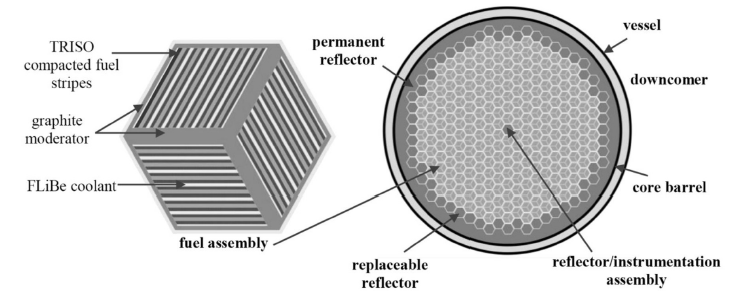
\includegraphics[width=0.9\linewidth]{ahtr.png} 
    \caption{FHR core configuration and fuel element \cite{ramey_monte_2018}.}
    \label{fig:ahtr}
\end{figure}

\subsection{Previous AHTR modeling efforts and challenges}
Modeling and simulation of the \gls{AHTR} design has been an ongoing effort 
since its conception in 2003 \cite{forsberg_molten-salt-cooled_2003}. 
The \gls{AHTR} core design differs significantly from the present \gls{LWR}-based 
nuclear power plants. 
These differences lead to modeling challenges and the need for verification and 
validation of modeling and simulation methods \cite{ramey_monte_2018}. 
Verification and validation of neutronics and thermal hydraulics tools' 
capability to successfully model the \gls{AHTR} design is a crucial step 
in support of licensure of the \gls{AHTR} design towards the eventual goal 
of deployment \cite{rahnema_phenomena_2019,rahnema_current_2015}. 
Several neutronic studies have been completed along the way to the current 
\gls{AHTR} design \cite{ramey_monte_2018,holcomb_fluoride_2013,greene_pre-conceptual_2010}. 
These efforts have shed light on the technical challenges facing the \gls{AHTR} design. 

In an effort to understand the challenges of \gls{FHR} materials, 
modeling the neutronics and thermal hydraulics in 
both plate and pebble fuelled \glspl{FHR}, a university-led Integrated 
Research Project \cite{zhang_integrated_2019} was conducted. 
During the research project, a panel of subject matter experts came together to 
generate a \gls{PIRT} by identifying phenomena and ranking their importance.
The \gls{PIRT} identifies areas in which additional research is needed to better 
understand important phenomena for adequate future modelling 
\cite{rahnema_phenomena_2019}. 
The phenomena identified as requiring further research are included in 
Table \ref{tab:phenomena}. 

\begin{table}[]
    \centering
    \onehalfspacing
    \caption{\gls{PIRT} identified \gls{FHR} physical phenomena requiring further research 
    \cite{rahnema_phenomena_2019}.}
	\label{tab:phenomena}
    \small
    \begin{tabular}{l|l}
    \hline
    \textbf{Category} & \textbf{Phenomena} \\ \hline
    Fundamental cross section data & - Moderation in FliBe \\
    & - Thermalization in FliBe \\
    & - Absorption in FliBe \\
    & - Thermalization in carbon \\
    & - Absorption in carbon \\ \hline
    Material Composition & - Fuel particle distribution \\ \hline
    Computational Methodology & - Solution Convergence \\ 
    & - Granularity of depletion regions \\
    & - Multiple heterogeneity treatment for generating multi-group \\ 
    & cross sections \\
    & - Selection of multi-group structure \\
    & - Boundary conditions for multi-group cross section generation \\ \hline 
    General Depletion & Spectral history \\ \hline 
    \end{tabular}
    \end{table}

The \gls{AHTR} has a complex core design due to the multiple heterogeneity present 
in the fuel introduced by presence of \gls{TRISO} particles embedded in plates 
\cite{ramey_monte_2018,rahnema_phenomena_2019}.
Accurately modeling the \gls{FHR}'s complex geometry with individual \gls{TRISO}
particle fidelity is necessary to obtain detailed reference power distributions 
to assess the accuracy of lower-fidelity models.
However, it is challenging, particularly for deterministic codes which 
use multigroup cross sections and traditional homogenization methods
\cite{ramey_monte_2018}. 
These traditional homogenization methods are insufficient to capture the correct physics 
in \glspl{FHR}, due to the multiple heterogeneity \cite{ramey_monte_2018}. 
In the \gls{AHTR}, single and multiple slab homogenization decreased computation time 
by 10, however they introduce a nontrivial error of $\sim$3\%
\cite{ramey_monte_2018,cisneros_neutronics_2012}.
Core physics parameters with acceptable uncertainty must be calculated to determine 
the feasibility and safety of the \gls{AHTR} design.
For Monte Carlo codes, statistical uncertainties must be reduced by increasing 
the number of neutron histories, however this comes at an increased 
computational cost.

Another technical challenge faced by the \gls{AHTR} design is the uncertainty of 
the graphite and carbonaceous moderator material properties: densities, temperatures
and thermal scattering data.
Also, the thermal scattering data ($S(\alpha,\beta)$ matrices) for the bound 
nuclei in the \gls{FLiBe} salt are lacking \cite{ramey_monte_2018}. 
Upon examination of the thermal scattering behavior of solid \gls{FLiBe}
\cite{mei_investigation_2013} and liquid \gls{FLiBe} \cite{zhu_thermal_2017}, 
it was observed that the bound and free atom cross section of \gls{FLiBe} are 
identical above 0.1eV and diverges below 0.01eV. 
This means that the use or absence of thermal scattering data will impact the 
accuracy of the results \cite{ramey_monte_2018}. 

\subsection{AHTR Benchmark}
In an effort to address and further understand the technical challenges described 
in the previous section, in 2019 the OECD-NEA initiated a benchmark to assess the 
state of the art modelling and simulation capabilities for \glspl{FHR} with 
\gls{TRISO} fuel embedded in fuel plates ("planks") of hexagonal fuel elements
\cite{noauthor_fluoride_nodate}. 
The benchmark plans to have three phases, starting from a single fuel element 
simulation without burnup, gradually extending to full core depletion and feedback. 
The overarching objective of the benchmark is to identify applicability, accuracy, 
and practicality of the current methods and codes to assess the current state 
of the art of \gls{FHR} simulation and modeling \cite{petrovic_preliminary_2021}. 
The benchmark also enables the cross-verification of codes and methodologies for the 
challenging \gls{AHTR} geometry, which is especially useful since applicable reactor 
physics experiments that may be used for validation of codes are scarce  
 \cite{petrovic_fhrahtr_2019,petrovic_preliminary_2021}. 
A detailed description of the phases of the benchmark and the results to date 
are described in Chapter \ref{chap:fhr-benchmark}. 

\section{Additive Manufacturing}
\gls{AM} is the formalized termed for what used to be called rapid prototyping 
and what is popularly called 3D printing \cite{gibson_additive_2014}. 
The basic principle of \gls{AM} is that a model is initially generated using a
\gls{3D CAD} system and is fabricated directly without the need for process 
planning. 
In \gls{AM}, the parts are made by adding materials in layers, each layer is a 
thin cross-section of the \gls{3D CAD} designed part, as opposed 
to subtractive manufacturing methods such as traditional machining
\cite{standard_standard_2012}. 
All commercialized \gls{AM} machines to date use a layer-based approach, and 
the major ways that they differ are in the materials that can be used, 
how the layers are created, and how the layers are bonded to each other
\cite{gibson_additive_2014}.
These major differences will determine the following factors: accuracy of the 
final part, its material and mechanical properties, time required to manufacture 
the part, the need for post-processing, size of \gls{AM} machine, and overall 
cost of the machine and the process \cite{gibson_additive_2014}. 
Initially, \gls{AM} was used to manufacture prototypes. 
However, with improvements in material properties, accuracy and overall quality 
of \gls{AM} output, the applications for \gls{AM} expanded, to the 
current point in which some industries build parts for direct assembly purposes
\cite{uriondo_present_2015}.  
Furthermore, using \gls{AM} in conjunction with other technologies, such as 
high-power laser technology, has enabled the use of \gls{AM} technology 
to manufacture parts made from a variety of metals \cite{gibson_additive_2014}. 

\subsection{Application of Additive Manufacturing to Nuclear Reactor Core Components}
\label{sec:am}
\gls{AM} has progressed rapidly in the last 30 years from rapid design protoyping 
with polymers in the automotive industry to scale production of metal components.  
Examples include Boeing using \gls{AM} to reduce the 979 Dreamliner's weight 
\cite{noauthor_printed_2017} and General Electric using \gls{AM} to produce fuel 
injection nozzles \cite{noauthor_transformation_2018}. 
The most common metal \gls{AM} technologies, \gls{SLM}, \gls{EBM}, \gls{L-DED}, 
and binder jetting, are not currently used to manufacture nuclear power plant parts. 
Wide-spread adoption of these methods in the nuclear industry could drastically 
reduce fabrication costs and timelines, combine multiple systems and assembled 
components into single parts, increase safety and performance by tailoring 
local material properties, and allow for redesigning of geometries for optimal 
load paths \cite{simpson_considerations_2019}. 
Many generation IV advanced reactor concepts have complex geometries, 
such as hex-ducts for sodium-cooled fast reactors, which are costly and difficult 
to fabricate using common processing techniques. 
Traditional manufacturing routes also restrict the viable geometries for 
reactor designers \cite{sridharan_performance_2019}. 
In summary, the main benefits of using \gls{AM} for reactor core components is that 
we are no longer geometrically constrained by conventional fuel manufacturing, 
and can further optimize and improve fuel geometries to enhance fuel performance and 
safety with the added benefit of lower cost \cite{bergeron_early_2018}. 

There has been experimental work done in the nuclear materials field towards 
demonstration of \gls{AM} of nuclear fuel and structural core materials. 
Bergeron et al \cite{bergeron_early_2018} successfully demonstrated additively 
manufacturing thorium dioxide using a stereolithography-based 3D printer 
and photopolymer resin. 
The high-density thorium dioxide objects were printed and sintered to densities 
of $\sim90\%$ \cite{bergeron_early_2018}. 
Rosales et al \cite{rosales_characterizing_2019} conducted a feasibility study 
of direct routes to fabricate dense uranium silicide ($U_3Si_2$) fuel pellets 
using the \gls{INL} invented \gls{AMAFT}. 
$U_3Si_2$ is an accident-tolerant nuclear fuel candidate due to its promising 
high uranium density and improved thermal properties. 
Its current metallurgical fabrication process is expensive and long, the goal of
\gls{AMAFT} is to fabricate $U_3Si_2$ at a lower cost, in a timely and
commercially-reliable manner \cite{rosales_characterizing_2019}.  
Sridharan et al \cite{sridharan_performance_2019} demonstrated the application of
the laser-blown-powder \gls{AM} process to fabricate \gls{FM} steel, a type of 
steel commonly used for cladding and structural components in nuclear reactors. 
Koyanagi et al \cite{koyanagi_additive_2020} presented the current status of 
\gls{AM} technology for manufacturing nuclear-grade \gls{SiC} materials, they 
demonstrated that combinations of \gls{AM} techniques and traditional \gls{SiC} 
densification methods enabled new designs of \gls{SiC} components with complex shapes. 
\gls{SiC} has excellent strength at elevated temperatures, chemical inertness, 
relatively low neutron absorption, and stability under neutron irradiation up 
to high doses \cite{sauder_ceramic_2014, snead_handbook_2007,koyanagi_additive_2020} 
which make it suitable for many applications in nuclear systems such as fuel cladding, 
constituents of fuel particles \cite{snead_handbook_2007} and pellets
\cite{terrani_progress_2015}, core structural components in fission reactors 
\cite{sauder_ceramic_2014}. 

\section{Nuclear Reactor Design Optimization}
The practice of nuclear reactor optimization has been around since the conception of 
nuclear reactors. 
Optimization has been applied to nuclear reactor design, reactor reloading 
patterns, and the nuclear fuel cycle.  
In the proposed work, we will focus on the optimization of nuclear reactor 
core design. 
Previous efforts towards nuclear reactor core design optimization include the use 
of deterministic and stochastic optimization techniques, and these optimization 
methods coupled with surrogate models. 

Deterministic optimization methods usually start from a random guess solution, 
thereafter the algorithm suggests a search direction based on applying local 
information to a pre-specified transition rule. 
The best solution becomes the new solution and the above procedure is continued 
for a number of times \cite{deb_multi-objective_2001}. 
Drawbacks of deterministic methods include: algorithms tend to get stuck to a 
suboptimal solution and an algorithm efficient in solving one type of problem, 
may not be efficient in solving a different problem \cite{deb_multi-objective_2001}. 
Stochastic optimization methods find globally optimal solutions more reliably. 
Evolutionary algorithms and simulated annealing are examples of stochastic 
optimization algorithms. 

The complexity of a nuclear reactor results in reactor design optimization 
being a multi-objective design problem requiring a tradeoff between desirable 
attributes \cite{byrne_evolving_2014,simon_sciences_2019}. 
When multiple conflicting objectives are important, there is no single optimum 
solution which simultaneously optimizes all objectives. 
Instead, the multi-objective optimization problem's outcome is a set of optimal 
solutions with a varying degree objective values \cite{deb_multi-objective_2001}. 
For a multi-objective problem like reactor design optimization, 
an ideal multi-objective optimization method should find widely spread solutions 
in the obtained non-dominated front \cite{deb_multi-objective_2001}, concluding 
that stochastic methods are ideal. 

Recent efforts towards nuclear reactor optimization have relied heavily on 
stochastic methods such as simulated annealing and evolutionary algorithms, 
with occasional stochastic-deterministic hybrid methods. 
Sacco et al \cite{sacco_two_2006,sacco_metropolis_2008} used stochastic 
optimization techniques similar to simulated annealing, and a 
deterministic-stochastic hybrid optimization technique
that combined one of the stochastic simulated annealing methods with the 
deterministic Nelder–Mead Simplex algorithm to optimize reactor dimensions, 
enrichment, materials etc., in order to minimize the average peak factor in a 
three-enrichment-zone reactor. 
Odeh et al \cite{odeh_core_2016} used the simulated annealing stochastic algorithm 
coupled with neutronics and thermal hyraulics codes, \gls{PARCS} and RELAP5, 
to develop an optimum core design for the \gls{NMR-50} to achieve a 10-year cycle length 
with minimal fissile loading. 
Kropaczek et al \cite{kropaczek_large-scale_2019} demonstrated the constraint 
annealing method, a highly scalable method based on the method of parallel 
simulated annealing with mixing of states \cite{kropaczek_constraint_2019}, for 
the solution of large-scale, multiconstrained problems in \gls{LWR} fuel cycle 
optimization. 
Peireira et al \cite{pereira_coarse-grained_2003,pereira_parallel_2008} 
used a coarse-grained parallel \gls{GA} and a niching \gls{GA}
to optimize the same problem as \cite{sacco_two_2006}. 
Kamalpour et al \cite{kamalpour_smart_2020} utilized the imperialist competitive 
algorithm, a type of evolutionary algorithm, to optimize a \gls{FCM} fuelled 
\gls{PWR} to extend the reactor core cycle length. 

Nuclear reactor optimization problems require the use of computationally 
extensive neutronics and thermal-hydraulics software to compute the objective 
function and constraints. 
In an effort to reduce computational cost of utilizing stochastic methods, 
multiple papers utilized optimization methods with surrogate models to replace 
high fidelity neutronics or thermal hydraulics simulations that typically 
require a high computational cost. 
Kumar et al \cite{kumar_new_2015} combined genetic algorithm optimization 
with regression splines surrogate model to optimize a reactor model for 
high breeding of U-233 and Pu-239 in desired power peaking limits, desired 
keff using the following parameters: radius of a fuel pin cell, isotopic enrichment 
of the fissile material in the fuel, mass flow rate of the coolant, and temperature 
of the coolant at the core inlet.
Betzler et al \cite{betzler_design_2019} developed a systematic approach to 
build a surrogate model to serve in place of high-fidelity computational 
analyses, they then leveraged the surrogate model with a simulated annealing 
optimization algorithm to generate optimized designs at a lower computational 
cost to understand the impact of design decisions on desired metrics for 
\gls{HFIR} \gls{LEU} core designs. 

The simulation annealing method uses a point-by-point approach, in which one
solution gets updated to a new solution in one iteration, which does not 
allow for advantages of parallel systems to be fully exploited. 
Finding an optimal solution with simulation annealing methods will take very 
long if high-fidelity codes are used to compute the objective function and 
constraints.
Therefore, using the simulation annealing method is only practical if a 
surrogate evaluation model is used as described in \cite{betzler_design_2019}.
Evolutionary algorithm method mimics nature's evolutionary principles to drive 
its search towards an optimal solution. 
Contrary to a single solution per iteration in deterministic and the stochastic 
simulation annealing methods, \glspl{EA} use a population of solutions in each 
iteration \cite{deb_multi-objective_2001}. 
With the affordability and availability of parallel computing systems, the 
evolutionary algorithm optimization method stands out as an optimization method 
that easily and conveniently exploits parallel systems. 
Therefore, in this proposed work, we will utilize the evolutionary algorithm 
optimization method. 

\subsection{Impact of additive manufacturing on nuclear reactor design 
optimization}
In section \ref{sec:am}, we discussed how with the advancements of \gls{AM} 
for reactor core components, reactor designers are no longer geometrically 
constrained by conventional fuel manufacturing, and can further optimize and 
improve fuel geometries to enhance fuel performance and safety. 
Reactor design objectives remain consistent with past objectives, such as minimizing 
fuel amount, minimizing maximum fuel temperature for a given power level. 
However, we can now approach the nuclear design problems with truly arbitrary 
geometries, no longer limited by traditional geometric shapes that are 
easy to manufacture with traditional processes: slabs as fuel plates, cylinders 
as fuel rods, spheres as fuel pebbles, axis-aligned coolant channels, etc  
\cite{sobes_artificial_2020}.
Therefore, this has opened the door for re-examination of optimization in 
completely new way, determining the optimal arbitrary geometry for a given objective 
function \cite{sobes_artificial_2020} with a much smaller set of constraints. 

With a substantial increase and change in the design space of an arbitrary 
geometry, it becomes time consuming for human reactor designer to completely 
explore the design space to find optimal geometries. 
Instead, we can leverage \gls{AI} to effectively explore the large design space 
in a timely manner to find global optimal designs. 
\gls{AI} would not replace the human reactor designer, but will shift the 
human designer's focus away from conjecturing good geometries to defining 
design criteria to find optimal designs \cite{sobes_artificial_2020}. 
Therefore, when the human designer changes the reactor criteria, the \gls{AI} 
model will easily adapt and produce new global optimal designs to fit the new 
criteria.  

\section{Evolutionary Algorithms}
Evolutionary algorithms have proved amenable to \gls{HPC} solution and 
scalable to tens of thousands of processors \cite{kropaczek_constraint_2019}
%\chapter{Fluoride-Salt-Cooled High-Temperature Reactor Benchmark}
\label{chap:fhr-benchmark}
% Main Gist 
% - The work I did for the FHR Benchmark
% Structure 
% - Specifications of benchmark problem
% - Results from benchmark
% Appendix? 
% - More details about the geometry 

\glspl{FHR} use \gls{TRISO} fuel and a low-pressure liquid fluoride-salt coolant.
\gls{FHR} technology combines \gls{FLiBe} coolant from \glspl{MSR} and 
\gls{TRISO} particles from \glspl{VHTR} to enable a reactor with 
low operating pressure, large thermal margin, and accident-tolerant 
qualities.
Within the \gls{FHR} reactor class, \glspl{AHTR} have plate-based fuel in a hexagonal 
fuel assembly. 
To address the \gls{AHTR} modeling challenges, described in Chapter 
\ref{chap:lit-review}, such as multiple heterogeneity and material cross-section 
data, the \gls{OECD}-\gls{NEA} and \gls{Georgia Tech} initiated the \gls{FHR} 
benchmark for the \gls{AHTR} design in 2019 \cite{noauthor_fluoride_nodate}. 
In section \ref{sec:fhr}, I gave an \gls{FHR} concept overview, 
a \gls{AHTR} design description, a review of previous efforts 
towards modeling these designs, and how these efforts led to the benchmark
initiation. 

The three-phase \gls{FHR} benchmark begins  with a single fuel assembly 
simulation without burnup and gradually extends to full core depletion. 
Table \ref{tab:phases} outlines the complete and incomplete benchmark phases.

\begin{table}[H]
    \centering
    \onehalfspacing
    \caption{\acrfull{FHR} benchmark Phases \cite{noauthor_fluoride_nodate}.}
	\label{tab:phases}
    \footnotesize
    \begin{tabular}{lclc}
    \hline 
    \textbf{Phases}& \textbf{Sub-phases} & \textbf{Description} & \textbf{Completed?} \\
    \hline
    \multirow{ 3}{5cm}{\textbf{Phase I: fuel assembly}} & I-A & 2D model, steady-state & \checkmark\\
    &I-B & 2D model depletion & \checkmark\\
    &I-C & 3D model depletion &\\
    \hline
    \multirow{2}{5cm}{\textbf{Phase II: 3D full core}}&II-A & Steady-state &\\
    &II-B & Depletion &\\
    \hline 
    \multirow{ 2}{5.5cm}{\textbf{Phase III: 3D full core with feedback \& multicycle analysis}}&III-A & Full core depletion with feedback &\\
    &III-B & Multicycle analysis &\\
    \hline
    \end{tabular}
\end{table}

In the subsequent sections, I will describe the benchmark's specifications for 
the \gls{AHTR} design and Phase I. Then, I will share our Phase I-A and I-B 
results generated with the OpenMC neutronics code \cite{romano_openmc_2013}. 

\section{Benchmark Specifications: AHTR Design}
Figure \ref{fig:reactor-schematic} shows the \acrfull{AHTR} schematic and a vertical 
cut of the reactor vessel. 
The \gls{AHTR} operates at 3400 MWt thermal power and 1400 MWe 
electric power \cite{varma_ahtr_2012}. 
\begin{figure}[]
    \centering
    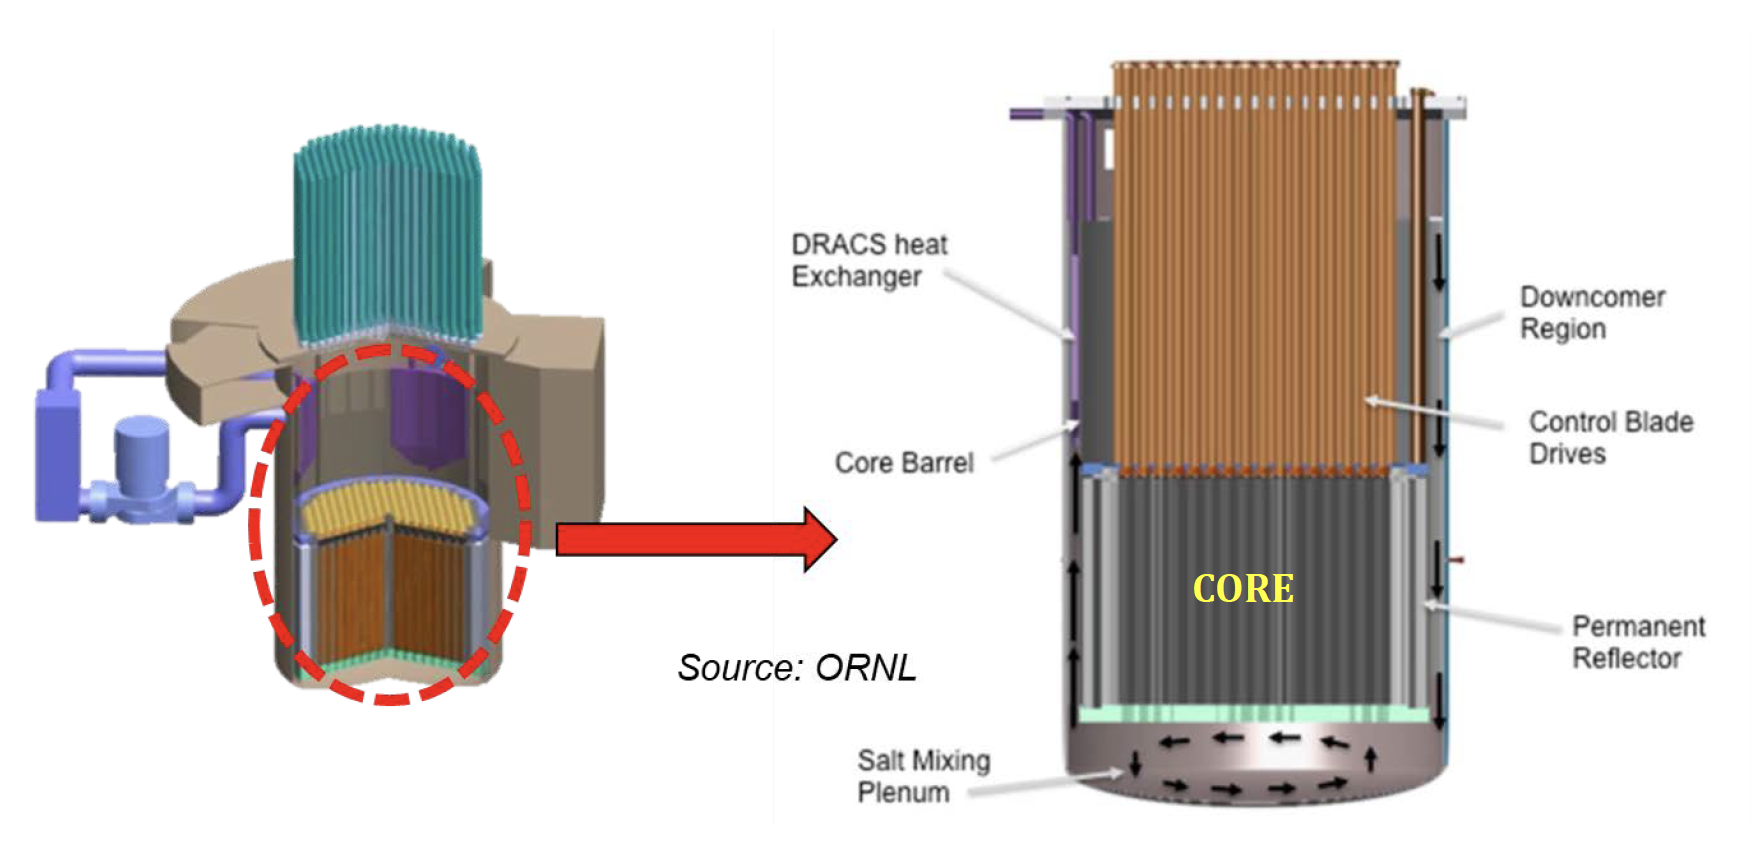
\includegraphics[width=\linewidth]{reactor-schematic.png} 
    \caption{\acrlong{AHTR} schematic (left) and vessel (right) reproduced from
    \cite{noauthor_fluoride_nodate}.}
    \label{fig:reactor-schematic}
\end{figure}
The exterior reactor vessel has a $10m$ diameter and contains an $8m$-diameter 
reactor core that contains 252 hexagonal fuel assemblies.
Each fuel assembly is $6m$ high with a $5.5m$ active core region, which contains
\gls{TRISO} particles, and $0.25m$ top and bottom non-fuelled reflector regions.
Figure \ref{fig:ahtr}, from Chapter \ref{chap:lit-review}, shows a single 
hexagonal fuel assembly geometry and the arrangement of all assemblies in the core.
The dimensions specified are room temperature dimensions. 
The benchmark's phases I and II use room temperature dimensions while phase III 
will address dimensional changes brought about by temperature expansion. 
Figure \ref{fig:ahtr-fuel-assembly} shows a detailed 2D view of the 
\gls{AHTR}'s hexagonal fuel assembly. 
\begin{figure}[]
    \centering
    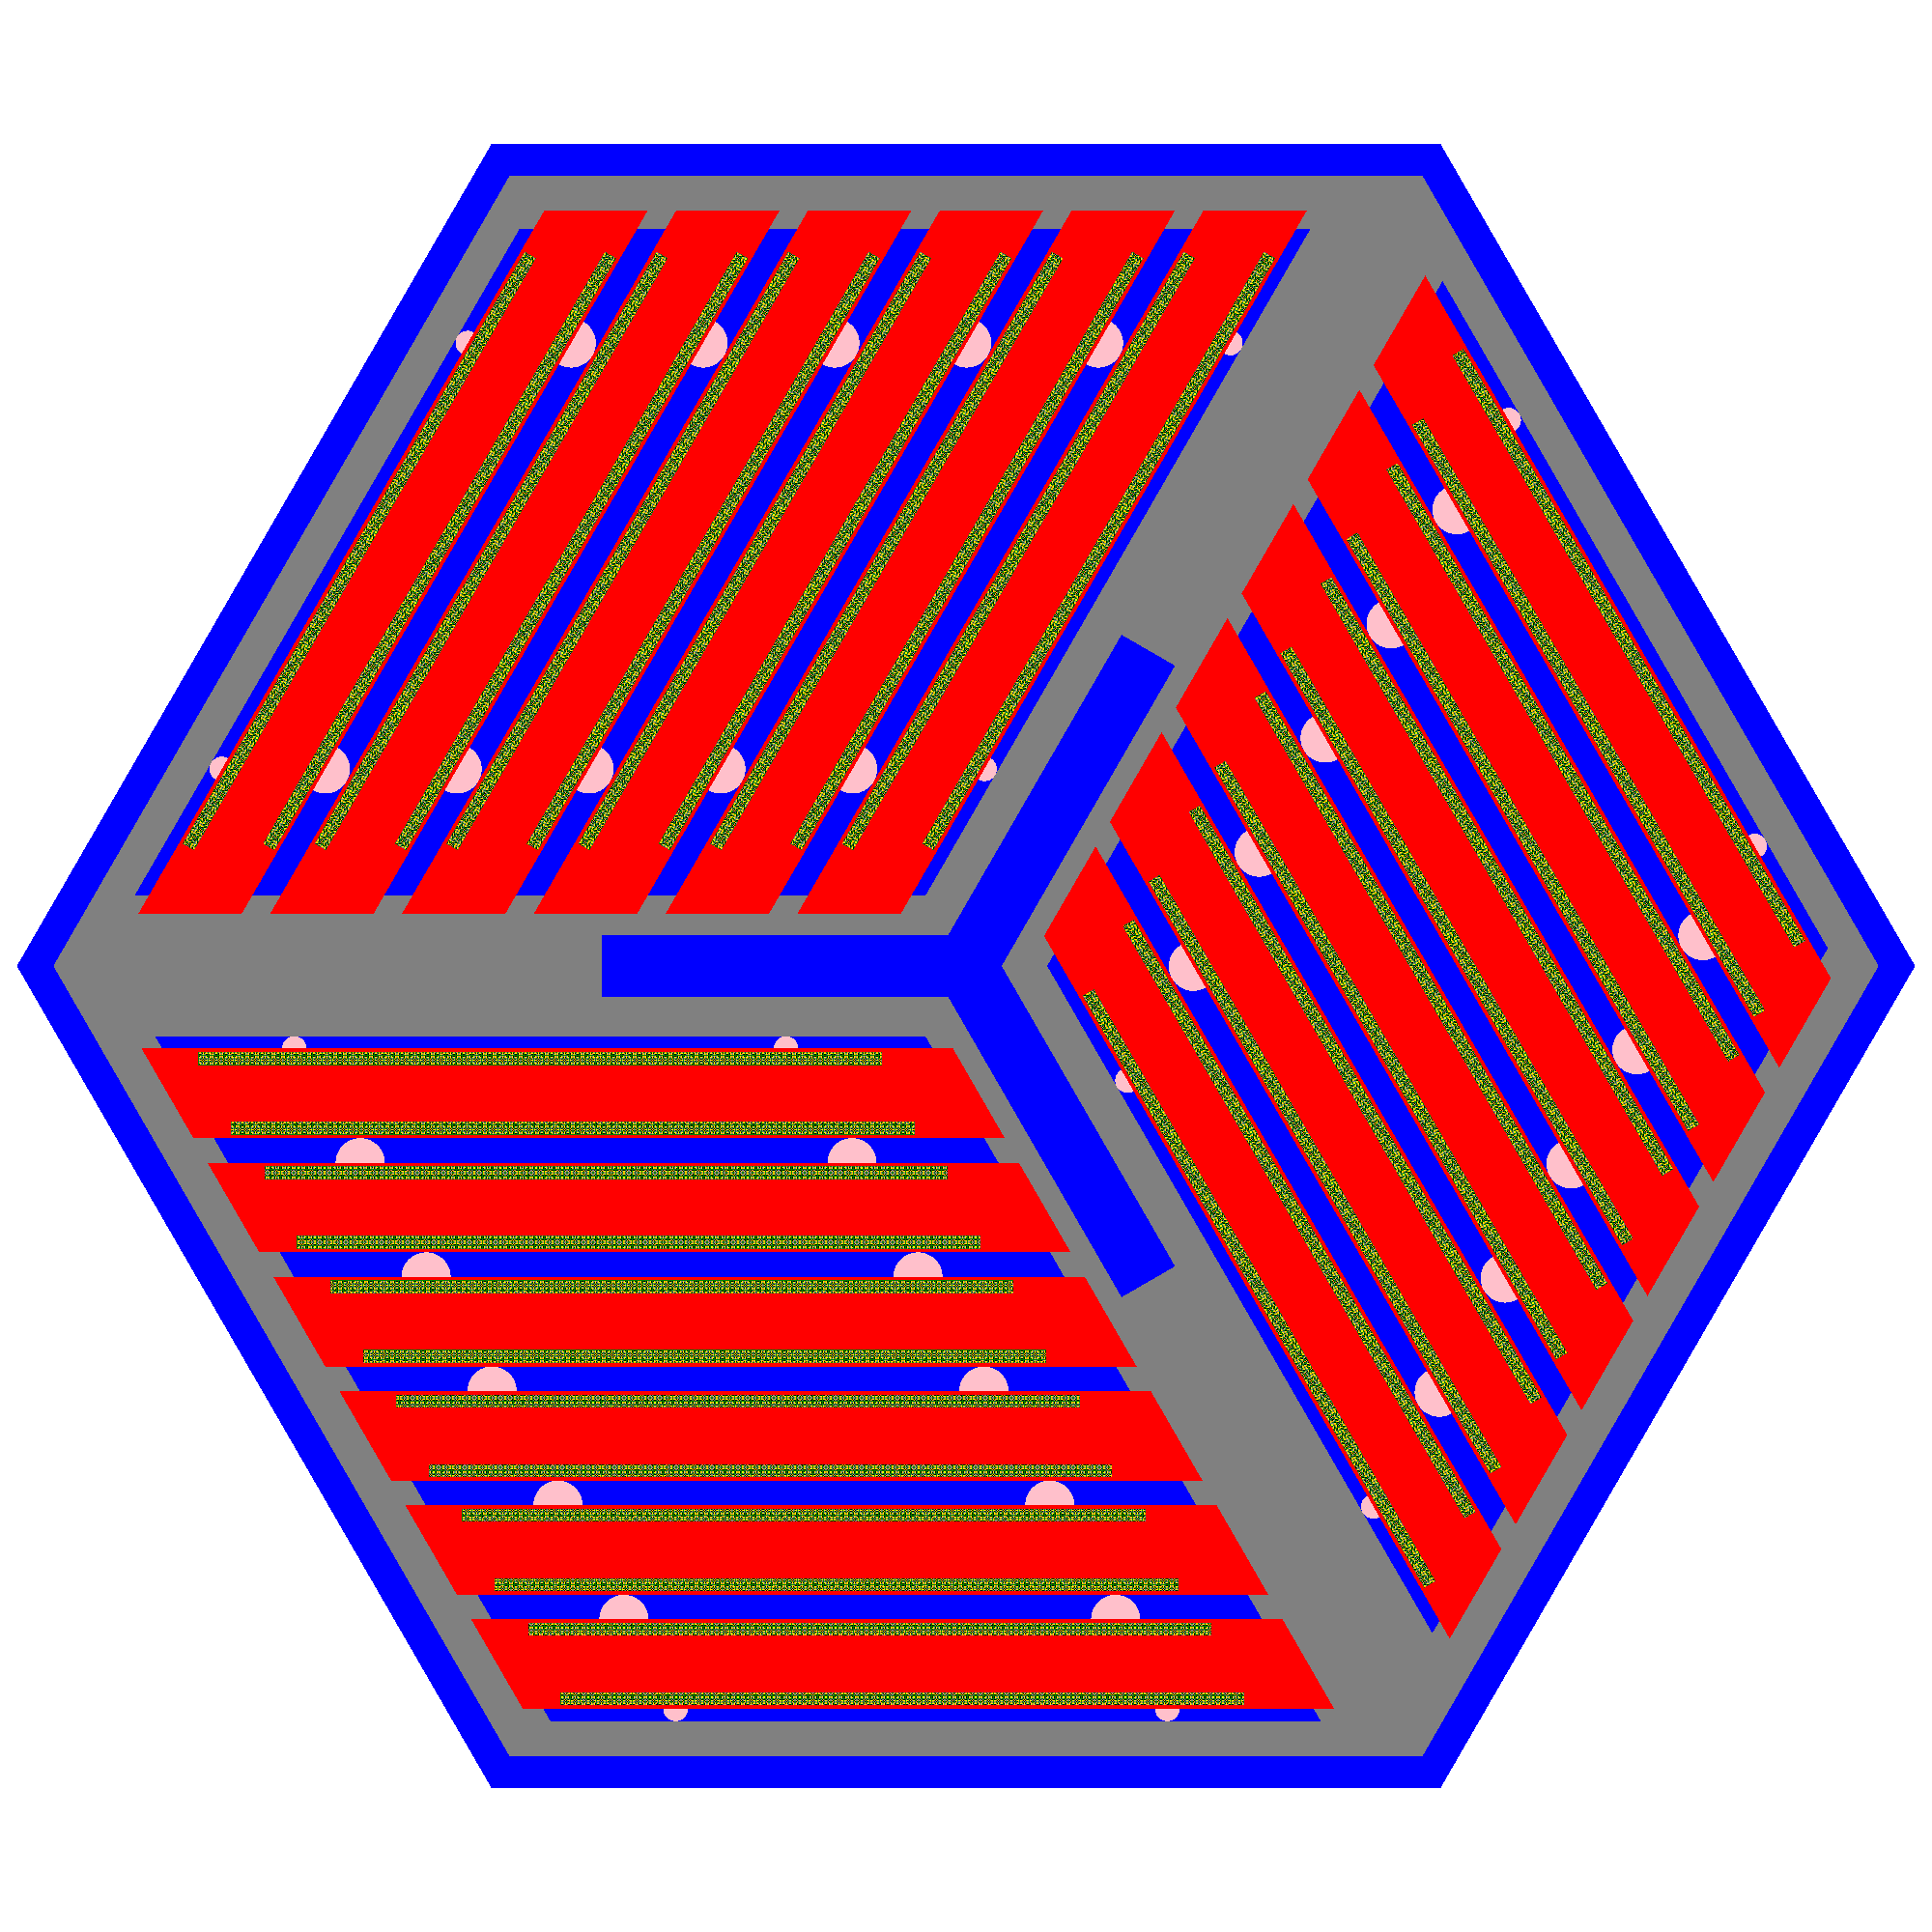
\includegraphics[width=0.9\linewidth]{ahtr-fuel-element.png} 
    \resizebox{0.4\textwidth}{!}{
        \fbox{\begin{tabular}{ll}
            \textcolor{fhrblue}{$\blacksquare$} & FLiBe \\
            \textcolor{fhrgrey}{$\blacksquare$} & Graphite (Fuel Structure)\\
            \textcolor{fhrred}{$\blacksquare$} & Graphite (Fuel Plank) \\
            \textcolor{fhrgreen}{$\blacksquare$} & Graphite (Fuel Stripe) \\
            \textcolor{fhryellow}{$\blacksquare$} & TRISO particle \\
            \end{tabular}}}
    \caption{\acrlong{AHTR} fuel assembly with 18 fuel plates arranged in 
    three diamond-shaped sectors, with a central Y-shaped and external channel 
    graphite structure. Blue: FliBE coolant in between fuel assemblies and plates, 
    and in the control rod slot, Gray: graphite structural components, 
    Red: graphite fuel plank, Pink: graphite spacers, Green: graphite matrix 
    with embedded TRISO particles.}
    \label{fig:ahtr-fuel-assembly}
\end{figure}
The hexagonal fuel assembly consists of eighteen fuel-containing graphite planks 
arranged in three diamond-shaped sectors, with a external channel wrapper and 
structural Y-shape, made of C-C composite with extra notches to hold the fuel 
planks in place. 
The diamond-shaped sections have $120^\circ{}$ rotational symmetry with each other 
\cite{varma_ahtr_2012,ramey_monte_2018,noauthor_fluoride_nodate}. 
The fuel planks have semi-cylindrical spacers attached, their radius being 
equal to the coolant channel thickness. 
\gls{FLiBe} coolant fills the gaps between the fuel planks, and between 
assemblies (note: FliBe layer around the single assembly). 
The Y-shaped control rod slot at the center of the Y-shape structure contains 
\gls{FLiBe} coolant when the control blade is not in the slot (as seen in 
Figure \ref{fig:ahtr-fuel-assembly})
\cite{varma_ahtr_2012,ramey_monte_2018,noauthor_fluoride_nodate}.
For a single fuel assembly, the internal 120-degree rotational symmetry is 
represented by periodic boundary conditions, as seen in Figure \ref{fig:bc}. 
\begin{figure}[]
    \centering
    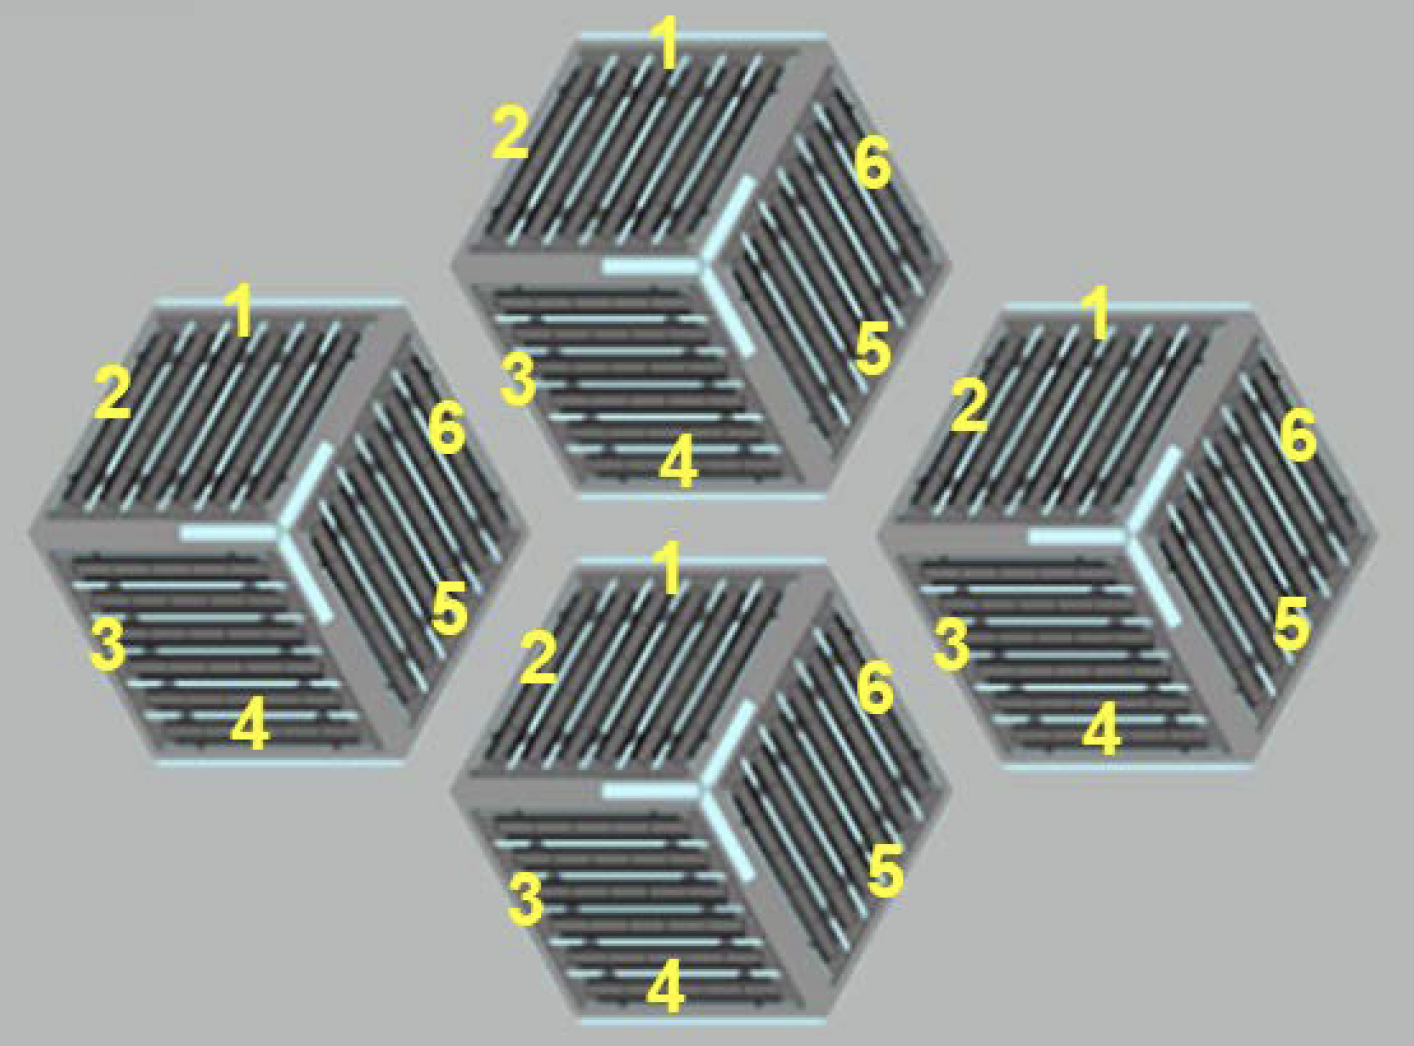
\includegraphics[width=0.7\linewidth]{bc.png} 
    \caption{Visualization of periodic boundary conditions for a single fuel 
    assembly in the \gls{AHTR}, reproduced from \cite{noauthor_fluoride_nodate}.}
    \label{fig:bc}
\end{figure}

Figure \ref{fig:ahtr-fuel-plank} magnifies a single fuel plank. 
Each fuel plank is made of an isostatically pressed carbon with fuel stripes 
on each outer side of the plank. 
\begin{figure}[]
    \centering
    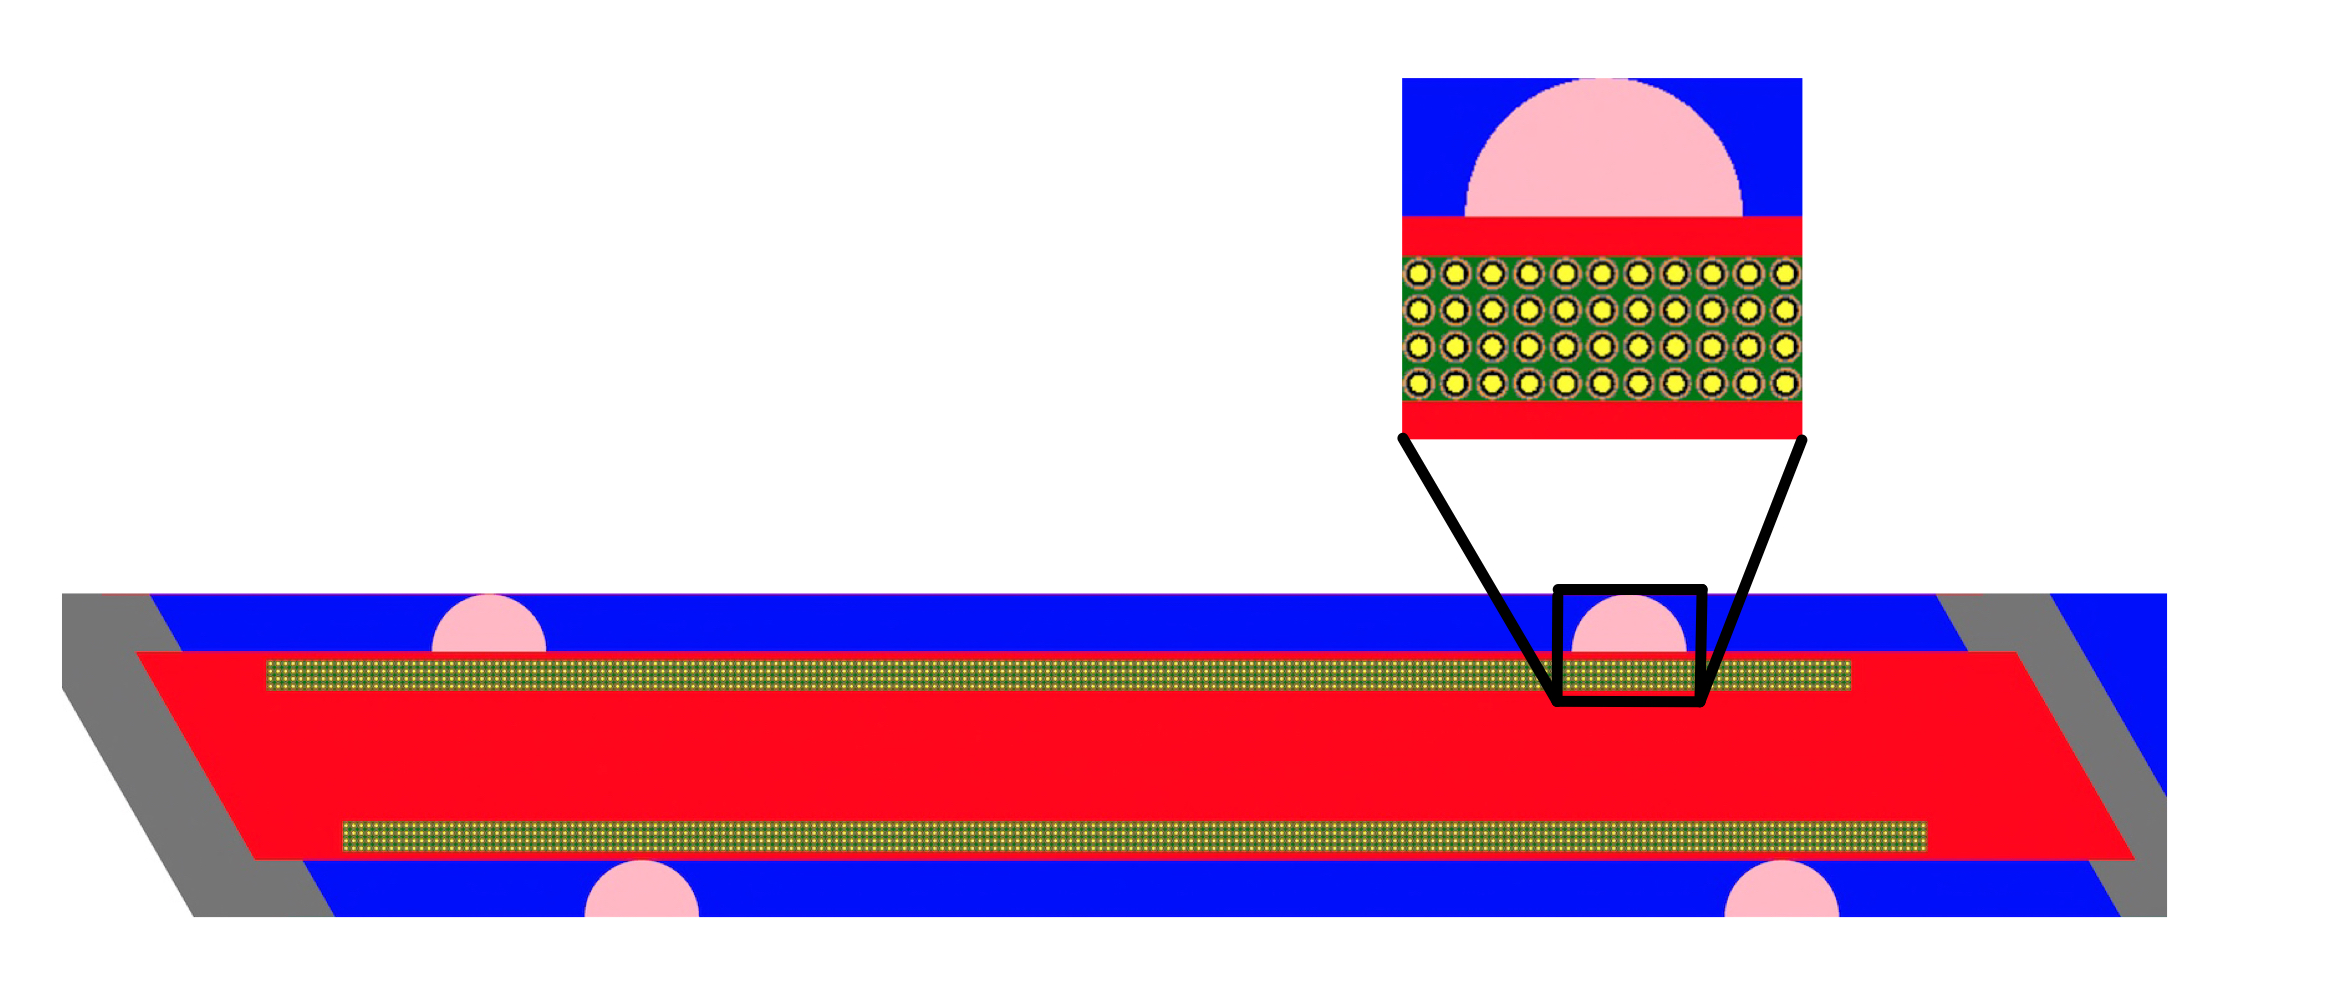
\includegraphics[width=\linewidth]{ahtr-fuel-plank.png} 
    \resizebox{0.4\textwidth}{!}{
        \fbox{\begin{tabular}{ll}
            \textcolor{fhrblue}{$\blacksquare$} & FLiBe \\
            \textcolor{fhrgrey}{$\blacksquare$} & Graphite (Fuel Structure)\\
            \textcolor{fhrred}{$\blacksquare$} & Graphite (Fuel Plank) \\
            \textcolor{fhrgreen}{$\blacksquare$} & Graphite (Fuel Stripe) \\
            \textcolor{fhryellow}{$\blacksquare$} & TRISO particle \\
            \textcolor{fhrpink}{$\blacksquare$} & Graphite (Spacer) \\
            \end{tabular}}}
    \caption{\acrlong{AHTR}'s fuel plank, with the magnification of 
    a spacer and segment of the fuel stripe with embedded TRISO particles.}
    \label{fig:ahtr-fuel-plank}
\end{figure}
The fuel stripes are prismatic regions composed of a graphite matrix filled with 
a cubic lattice of \gls{TRISO} particles with 40\% packing fraction. 
The lattice is 210 \gls{TRISO} particles wide in the x-direction, four particles 
deep in the y-direction, and 5936 particles tall in the z-direction. 
Figure \ref{fig:ahtr-triso} shows the \gls{TRISO} particle which contains five 
layers: oxycarbide fuel kernel, porous carbon buffer, inner pyrolytic carbon, 
silicon carbide layer, and the outer pyrolitic carbon. 
\begin{figure}[]
    \centering
    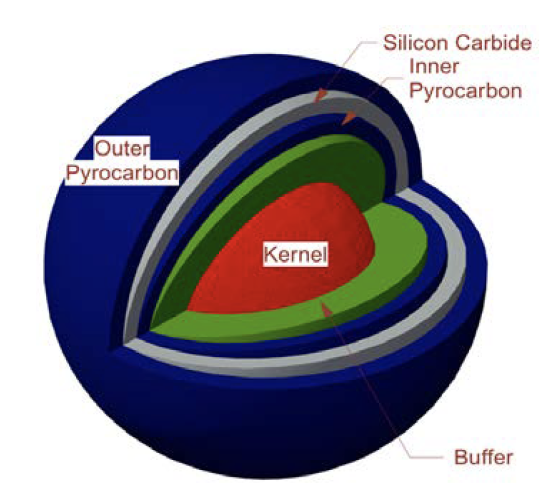
\includegraphics[width=0.6\linewidth]{ahtr-triso.png} 
    \caption{\acrlong{AHTR}'s TRISO particle schematic reproduced from 
    \cite{noauthor_fluoride_nodate}.}
    \label{fig:ahtr-triso}
\end{figure}

For reactivity control, burnable poisons and control rods are included in 
some configurations of the \gls{AHTR}. 
The burnable poisons consist of europium oxide, $Eu_2O_3$, and have a discrete
or integral (dispersed) option. 
Figure \ref{fig:discrete-poison} shows the discrete option in which small 
spherical $Eu_2O_3$ particles are stacked axially at five locations in each 
fuel plank. 
\begin{figure}[]
    \centering
    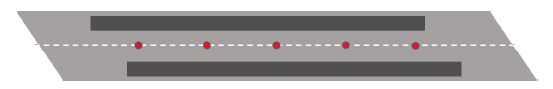
\includegraphics[width=\linewidth]{discrete-poison.png} 
    \caption{Placement of axial stacks of burnable poisons in the \acrlong{AHTR} 
    \cite{noauthor_fluoride_nodate}.}
    \label{fig:discrete-poison}
\end{figure}
In the integral option, $Eu_2O_3$ is homogenously mixed with the fuel plank 
graphite matrix (including the graphite in fuel stripes matrix and plank ends 
indented to structural sides, but excluding the graphite in spacers and 
graphite in TRISO particles). 
Each control rod is uniformly composed of \gls{MHC} and is inserted into the 
Y-shaped control rod slot where it displaces the \gls{FLiBe} that occupies the 
slot (shown in Figure \ref{fig:ahtr-fuel-assembly}). 

\section{Benchmark Specifications: Phase I}
\label{sec:phase1}
The \gls{FHR} benchmark's Phase I consists of a steady-state 2D model 
(Phase I-A) and depletion (Phase I-B) of one \gls{FHR} fuel assembly. 
The benchmark required the following results for Phases I-A and I-B:
\begin{enumerate}[label=(\alph*)]
    \item effective multiplication factor 
    \item reactivity coefficients ($\beta_{eff}$, fuel Doppler coefficient, FLiBe 
    temperature coefficient, graphite temperature coefficient)
    \item tabulated fission source distribution by one-fifth fuel stripe
    \item neutron flux averaged over the whole model tabulated in three coarse energy groups
    \item neutron flux distribution in three coarse energy groups
    \item fuel assembly averaged neutron spectrum
\end{enumerate}
Next, I report the equations used to calculate these required results.  

\subsubsection{Reactivity Coefficients (b)}
Effective delayed neutron fraction ($\beta_{eff}$) is the fraction of delayed 
neutrons in the core. 
I assumed one energy group and six delayed groups for $\beta_{eff}$. 
Reactivity coefficient is the change in reactivity ($\rho$) of the material 
per degree change in the material's temperature (T). 
I calculated each reactivity coefficient and its corresponding uncertainty 
with these equations: 
\begin{align}
    \frac{\Delta \rho}{\Delta T} &= 
    \frac{\rho_{T_{high}}-\rho_{T_{low}}}{T_{high}-T_{low}} \ [\frac{pcm}{K}] \\
    \delta \frac{\Delta \rho}{\Delta T} &= 
    \frac{\sqrt{\delta (\rho_{T_{high}})^2+(\delta \rho_{T_{low}})^2}}{T_{high}-T_{low}} \ [\frac{pcm}{K}] 
\end{align}

\subsubsection{Fission Source Distribution / Fission Density (c)}
I calculated \gls{FD} with OpenMC's \texttt{fission} tally score (f) 
for each region divided by the average \texttt{fission} tally score of all the regions:
\begin{align}
    FD_i &=  \frac{f_i}{f_{ave}} \\
    \intertext{where}
    f_i &= \mbox{fission reaction rate in a single region [reactions/src]} \nonumber \\
    f_{ave} &= \mbox{average of all $f_i$ [reactions/src]} \nonumber
\end{align}
The uncertainty calculations for $FD_i$ and $f_{ave}$: 
\begin{align}
    \delta FD_i &= |FD_i| \sqrt{(\frac{\delta f_i}{f_i})^2+(\frac{\delta f_{ave}}{f_{ave}})^2} \\
    \delta f_{ave} &= \frac{1}{N}\sqrt{\sum_i^Nf_i^2} \\
    \intertext{where}
    N &= \mbox{No. of fission score values} \nonumber
\end{align}

\subsubsection{Neutron Flux (d, e, f)}
OpenMC's \texttt{flux} score is in [$\frac{neutrons\ cm}{src}$] units. 
For the benchmark, I converted flux to [$\frac{neutrons}{cm^2s}$] units
using the following equations:  

\begin{align}
    \Phi_c &= \frac{N \times \Phi_o}{V} \\
    N &= \frac{P\times\nu}{Q\times k} \\
    \intertext{where}
    \Phi_c &= \mbox{converted flux [$\frac{neutrons}{cm^2s}$]} \nonumber \\ 
    \Phi_o &= \mbox{original flux [$\frac{neutrons\ cm}{src}$]} \nonumber \\
    N &= \mbox{normalization factor [$\frac{src}{s}$]} \nonumber \\
    V &= \mbox{volume of fuel assembly [$cm^3$]} \nonumber \\
    P &= \mbox{power [$\frac{J}{s}$]} \nonumber \\
    \nu &= \mbox{$\frac{\nu_f}{f}$ [$\frac{neutrons}{fission}$]} \nonumber \\
    Q &= \mbox{Energy produced per fission [$\frac{J}{fission}$]} = \mbox{$3.2044 \times 10^{-11}$ J per $U_{235}$ fission} \nonumber \\
    k &= \mbox{$k_{eff}$ [$\frac{neutrons}{src}$]} \nonumber 
\end{align}
The flux standard deviation is: 
\begin{align}
    \delta \Phi_c = \Phi_c \times
    \sqrt{(\frac{\delta \Phi_o}{\Phi_o})^2+ (\frac{\delta \nu_f}{\nu_f})^2 
    + (\frac{\delta k}{k})^2 + (\frac{\delta f}{f})^2}
\end{align}
I calculated reactor power based on the given reference specific power 
($P_{sp}$) of 200 $\frac{W}{gU}$: 
\begin{align}
    P &= P_{sp} \times V_F \times \rho_F \times \frac{wt\%_{U}}{100} \\
    \intertext{where}
    V_F &= \mbox{volume of fuel [$cm^3$]} = \frac{4}{3} \pi r_f^3 \times N_{total} \nonumber \\
    r_f &= \mbox{radius of fuel kernel} \nonumber\\
    N_{total} &= \mbox{total no. of TRISO particles in fuel assembly} = 101 \times 210 \times 4 \times 2 \times 6 \times 3 \nonumber\\ 
    \rho_F &= \mbox{density of fuel [$g/cc$]} \nonumber \\
    wt\%_{U} &= \frac{at\%_{U235} \times AM_{U235} + at\%_{U238} \times AM_{U238}}{\sum (at\%_i \times AM_i)} \times 100 \nonumber\\
    AM &= \mbox{atomic mass} \nonumber
\end{align}

\subsection{Benchmark Specifications: Phase I-A}
For Phase I-A, the benchmark specifies that each participant must produce a 
steady-state 2D model of one fresh fuel assembly for nine cases
and report the required results listed in Section \ref{sec:phase1}.  
Table \ref{tab:phase1a-cases} describes each case. 
\begin{table}[H]
    \centering
    \onehalfspacing
    \caption{Description of the \acrlong{FHR} benchmark Phase I-A cases \cite{noauthor_fluoride_nodate}.}
	\label{tab:phase1a-cases}
    \footnotesize
    \begin{tabular}{p{0.05\textwidth}|p{0.95\textwidth}}
    \hline 
    \textbf{Case} & \textbf{Description} \\
    \hline
    1A & Reference case. Hot full power (HFP), with temperatures of 1110K for 
    fuel kernel and 948K for coolant and all other materials (including TRISO 
    particle layers other than fuel kernel). Nominal (cold) dimensions, 
    9 wt\% enrichment, no \gls{BP}, \glspl{CR} out.\\
    \hline
    2AH & \Gls{HZP} with uniform temperature of 948 K, 
    otherwise same as Case 1A. Comparison with Case 1A provides HZP-to-HFP power 
    defect.\\
    \hline 
    2AC & \Gls{CZP}. Same as Case 2AH, but with uniform temperature 
    of 773 K. Comparison with Case 2AH provides isothermal temperature coefficient.\\
    \hline
    3A & \gls{CR} inserted, otherwise same as Case 1A. \\
    \hline
    4A & Discrete europia \gls{BP}, otherwise same as Case 1A.\\
    \hline
    4AR & Discrete europia \gls{BP} and \gls{CR} inserted, otherwise same as 
    Case 1A. \\
    \hline
    5A & Integral (dispersed) europia \gls{BP}, otherwise same as Case 1A. \\
    \hline
    6A & Increased \gls{HM} loading (4 to 8 layers of \gls{TRISO}) decreased C/HM 
    ratio (from about 400 to about 200) and decreased specific power to 100 W/gU, 
    otherwise same as Case 1A.\\
    \hline 
    7A & Fuel enrichment 19.75 wt\%, otherwise same as Case 1A.\\
    \hline 
    \end{tabular}
\end{table}

\subsection{Benchmark Specifications: Phase I-B}
For Phase I-B, the benchmark specifies that each participant must produce 
depletion results for three cases: 1B, 4B, and 7B. 
These are the same as cases 1A, 4A, and 7A, but with depletion steps added. 
The benchmark assumes that depletion occurs only in the fuel and \glspl{BP} and 
that the depletion performs under the critical spectrum assumption. 

\section{Results}
Several organizations participated in the benchmark with various Monte Carlo
and Deterministic neutronics codes, such as Serpent \cite{leppanen_serpent_2014}, 
OpenMC \cite{romano_openmc_2013}, and WIMS \cite{lindley_current_2017}. 
\gls{UIUC} participated in the benchmark with the OpenMC Monte Carlo code 
\cite{romano_openmc_2013} and the ENDF/B-VII.1 material library 
\cite{chadwick_endf/b-vii.1_2011}.
The \texttt{fhr-benchmark} Github repository contains all the results submitted 
by \gls{UIUC} for the \gls{FHR} benchmark \cite{chee_arfcfhr-benchmark_2021}. 
The benchmark used a phased blind approach -- participants were asked to 
submit Phase I-A and I-B results without knowledge of other submissions. 
Petrovic et al. \cite{petrovic_preliminary_2021} describes the preliminary 
results of the benchmark results across several institutions and concludes 
that the overall observed agreement is satisfactory. 
In the subsequent sections, I will share the results obtained by \gls{UIUC}.  

\subsection{Results: Phase I-A}
Petrovic et al. \cite{petrovic_preliminary_2021} compared the effective 
multiplication factor ($k_{eff}$) for all participants and Phase I-A cases in 
the \gls{FHR} benchmark. 
They reported that the standard deviation between participants for each case 
was in the 231 to 514 pcm range, acceptable and notably close given a blind 
benchmark, assuring us that our Phase I-A results are acceptable and in agreement 
with other benchmark participants. 

Table \ref{tab:phase1a-cases} reports Phase I-A $k_{eff}$ and reactivity 
coefficients results. 
I ran the simulations on \gls{UIUC}'s BlueWaters supercomputer with 64 XE nodes, 
which each have 32 cores \cite{ncsa_about_2017}. 
To reduce $k_{eff}$'s statistical uncertainty to $\sim$10pcm, I ran each simulation 
with 500 active cycles, 100 inactive cycles, and 200000 neutrons. 
Each simulation took \gls{WCT} ranging from 2 to 5 hours. 
\begin{table}[H]
    \centering
    \onehalfspacing
    \caption{\acrlong{UIUC}'s \acrlong{FHR} Benchmark Phase I-A results 
    \cite{chee_arfcfhr-benchmark_2021}.}
	\label{tab:phase1a-results}
    \footnotesize
    \begin{tabular}{cp{2.7cm}cccccc}
    \hline
    \textbf{Case} & \textbf{Summary} & \textbf{WCT [hr]} & \textbf{$k_{eff}$}* & 
    \textbf{$\beta_{eff}$}** & 
    \textbf{Fuel} $\frac{\Delta \rho}{\Delta T}$ & 
    \textbf{FliBe} $\frac{\Delta \rho}{\Delta T}$ & 
    \textbf{Graphite} $\frac{\Delta \rho}{\Delta T}$\\
    \hline 
    1A & Reference &2.82&1.39389 & 0.006534 & -2.24$\pm$0.15 & -0.15$\pm$0.15 & -0.68$\pm$0.15\\
    2AH & \gls{HZP} &2.82&1.40395 & 0.006534 & -3.14$\pm$0.15 & -0.20$\pm$0.14 & -0.85$\pm$0.14\\
    2AC & \gls{CZP} &2.75&1.41891 & 0.006534 & -3.36$\pm$0.14 & -0.11$\pm$0.14 & 0.07$\pm$0.14\\
    3A & \gls{CR} &2.49&1.03147 & 0.006534 & -4.03$\pm$0.28 & -0.83$\pm$0.27 & -3.18$\pm$0.29\\
    4A & Discrete \gls{BP} &5.08&1.09766 & 0.006542 & -4.06$\pm$0.24 & -1.55$\pm$0.23 & -6.51$\pm$0.24\\
    4AR & Discrete \gls{BP} + \gls{CR} &4.59&0.84158 & 0.006553 & -5.60$\pm$0.49 & -1.78$\pm$0.46 & -10.44$\pm$0.47\\
    5A & Dispersed \gls{BP} &2.33&0.79837 & 0.006556 & -5.09$\pm$0.40 & -4.87$\pm$0.40 & -22.99$\pm$0.38\\
    6A & Increased \gls{HM} &3.52&1.26294 & 0.006556 & -4.46$\pm$0.19 & 0.16$\pm$0.20 & -0.39$\pm$0.20\\
    7A & 19.75\% Enriched &2.21&1.50526 & 0.006530 & -2.49$\pm$0.13 & -0.12$\pm$0.12 & -0.62$\pm$0.12\\
    \hline
    \multicolumn{5}{l}{* All $k_{eff}$ values have an uncertainty of 0.00010.} \\
    \multicolumn{5}{l}{** All $\beta_{eff}$ values have an uncertainty of 0.000001.} 
    \end{tabular}
\end{table}

Cases 2AH and 2AC are at zero power, meaning that the fuel assembly is exactly 
critical but not producing any energy. 
For both cases, $k_{eff}$ is higher than the reference Case 1A, which I attribute to 
lower fuel temperatures. 
At lower fuel temperatures, less doppler broadening occurs, 
resulting in less neutron capture, thus, increasing $k_{eff}$. 
As expected, $k_{eff}$ is lower for Cases 3A, 4AR, and 5A than reference case 
1A since these cases introduce burnable poisons and control rods to the fuel 
assembly. 
Also, as expected, $k_{eff}$ is higher for Case 7A than reference Case 1A, since 
it has a higher enrichment. 
However, Case 6A deviated from expectations with a lower $k_{eff}$ despite an increase 
in \acrlong{HM} loading. 
This behavior is due to reduced moderation and worsened fuel 
utilization brought about by self-shielding, demonstrating that an increase in 
fuel packing fraction does not always correspond with an increased $k_{eff}$. 

$\beta_{eff}$ increased by 10-20pcm for Cases 4A, 4AR, 5A, and 6A compared to
reference Case 1A due to the introduction of control rods and poisons that 
shift the average neutron velocity to higher values, resulting in decreased
thermal fission and increased fast fission \cite{torabi_neutronic_2018}.
Table \ref{tab:phase1a-results} reports that most of the temperature coefficients 
are negative, exemplifying the \gls{AHTR}'s passive safety behavior. 
Negative reactivity feedback results in a self-regulating reactor; if the reactor's 
power rises, resulting in temperature increase, the negative reactivity
reduces power. 

Figure \ref{fig:phase1a-c} shows the fission source distribution by 
one-fifth fuel stripe for Cases 1A and 3A. 
\begin{figure}[]
    \centering
    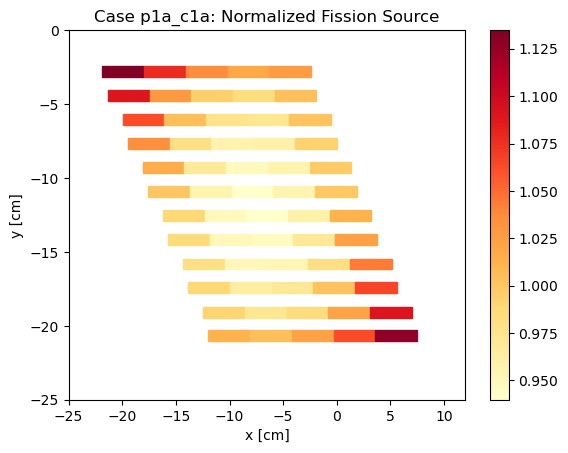
\includegraphics[width=0.52\linewidth]{p1a_c1a_c.png} 
    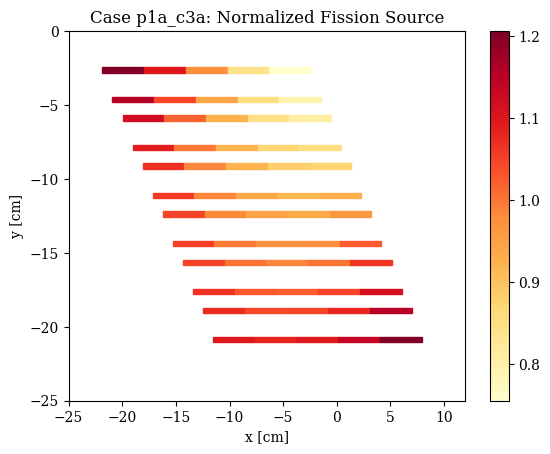
\includegraphics[width=0.52\linewidth]{p1a_c3a_c.png} 
    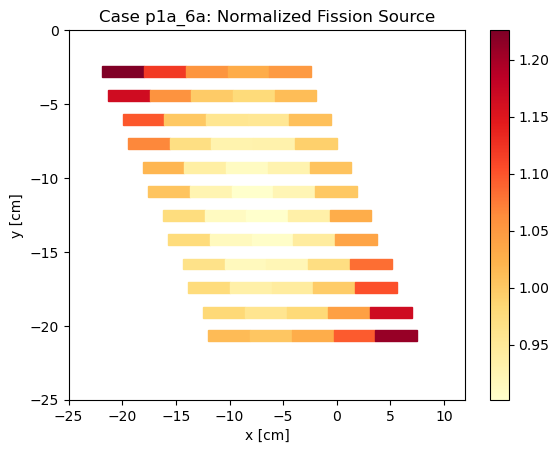
\includegraphics[width=0.52\linewidth]{p1a_6a_c.png} 
    \caption{Fission Source Distribution per one-fifth fuel stripe for 
    \acrlong{FHR} Benchmark's Phase I-A Case 1A (top), Case 3A (middle), 
    and Case 6A (bottom).}
    \label{fig:phase1a-c}
\end{figure}
Case 4AR has a similar fission source distribution as Case 3A since both 
cases have control rod insertion. 
All other cases have similar fission source distribution shape to Case 1A. 
For Case 1A, intuitively, I would assume that the highest fission source would 
occur in the center of the diamond fuel segment; however, the opposite is true. 
Power peaking occurs on exterior stripes and is minimum on the interior stripes.
Gentry et al. \cite{gentry_development_2016} reported similar power peaking 
phenomena towards the lattice cell's exterior closest to the Y-shaped carbon 
support structure where the thermal flux is most elevated. 
The lowest power is found in the interiors of the lattice tri-sections. 
This fission source distribution is caused by diminished resonance escape 
probability in the interior due to the higher relative fuel-to-carbon volume 
ratio. 
For Case 3A with an inserted control rod, the fission source is lower in 
the one-fifth stripes closer to the control rod.  
Cases 6A and 7A demonstrate a further diminished fission source in the interior 
stripes due to the higher fuel-to-carbon ratio.
This is seen in Figure \ref{fig:phase1a-c} in which case 1A and 6A have similar 
fission distribution shapes, but case 6A's has a bigger fission source value range. 

Figure \ref{fig:phase1a-d} shows the average neutron flux in the fuel assembly in 
three coarse energy groups. 
\begin{figure}[]
    \centering
    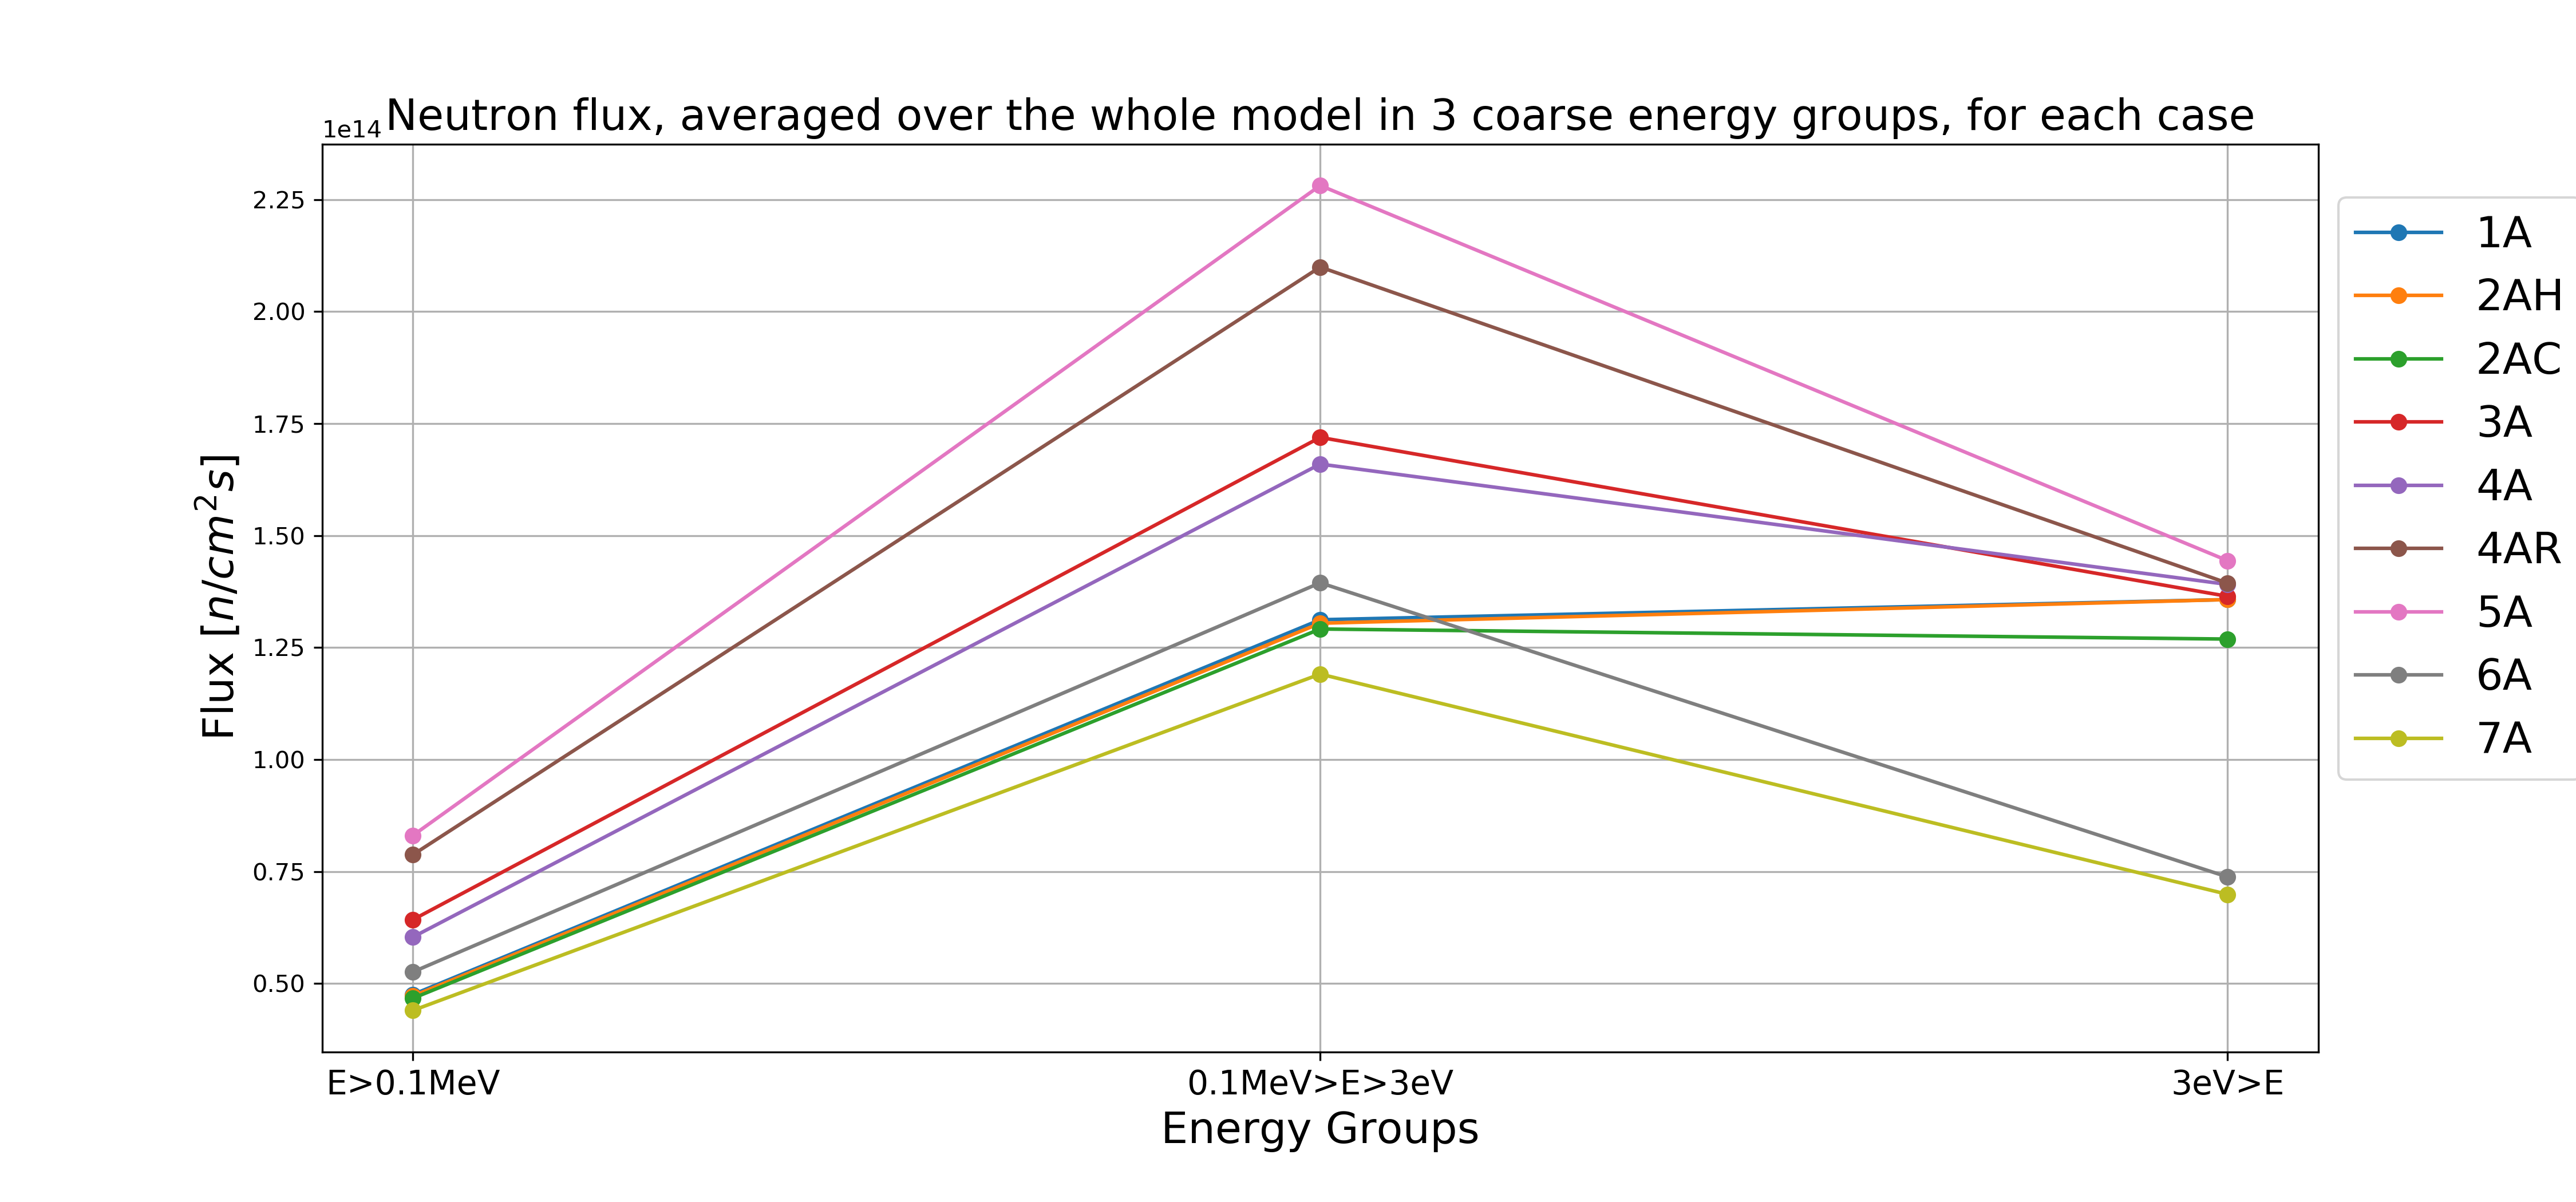
\includegraphics[width=\linewidth]{phase1a-d-flux.png} 
    \caption{\acrlong{FHR} Benchmark's Neutron flux, averaged over the whole 
    model, tabulated in three coarse energy groups for each Phase I-A case. }
    \label{fig:phase1a-d}
\end{figure}
Most of the cases have the most flux in the intermediate group, followed by 
the thermal group, and the least flux in the fast group.    
Figure \ref{fig:phase1a-e} shows the neutron flux distribution in a 100 $\times$ 
100 mesh for Cases 1A, 3A, and 6A for three coarse energy groups. 
\begin{figure}[]
    \centering
    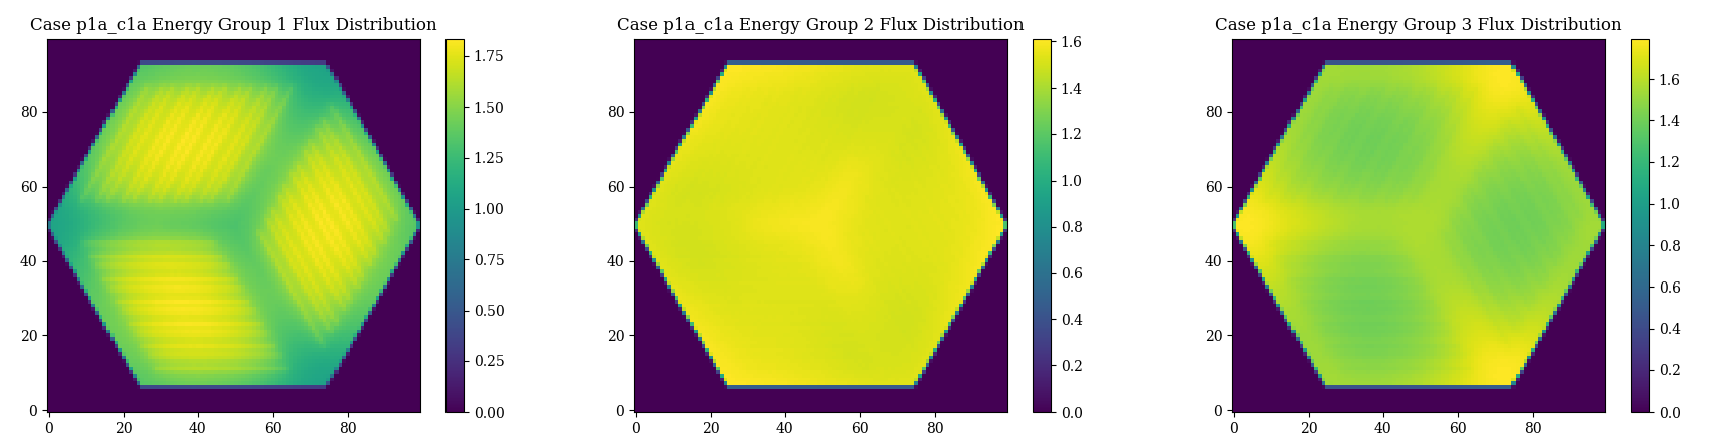
\includegraphics[width=\linewidth]{phase1a-e-c1a.png} 
    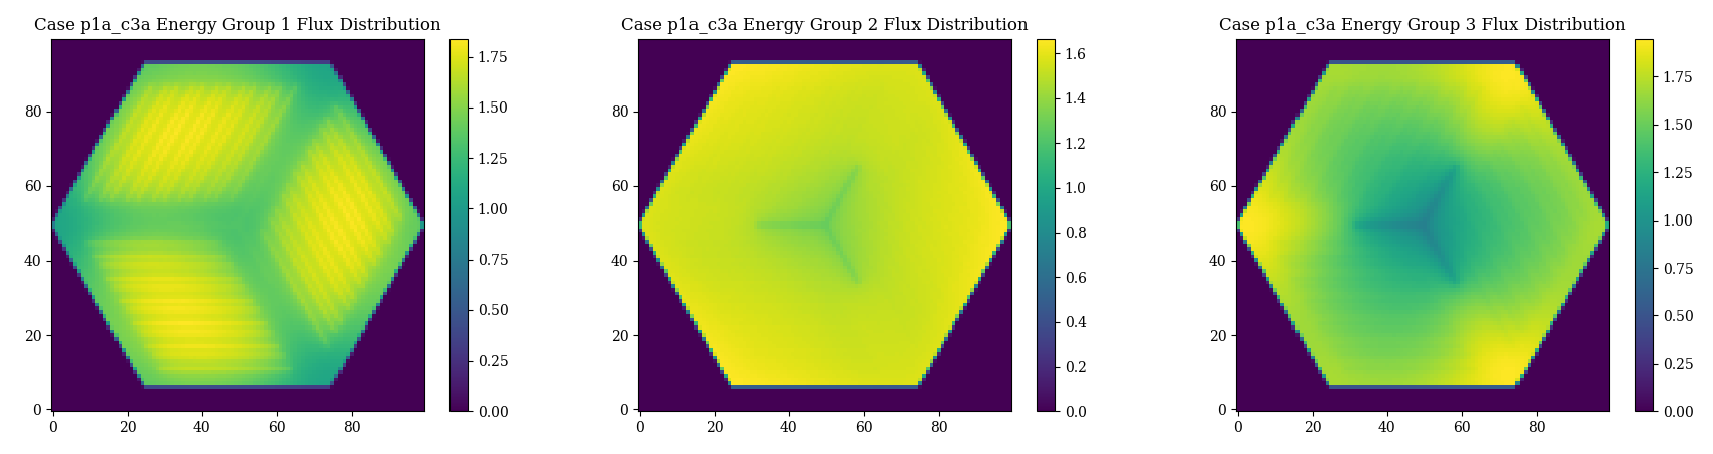
\includegraphics[width=\linewidth]{phase1a-e-c3a.png} 
    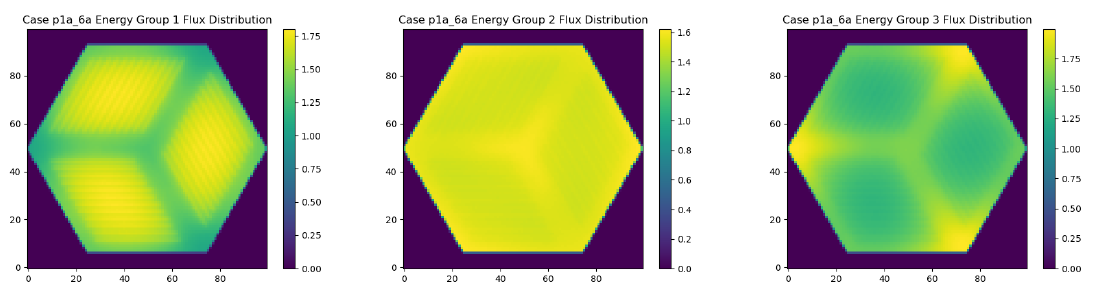
\includegraphics[width=\linewidth]{phase1a-e-c6a.png} 
    \caption{\acrlong{FHR} Benchmark's Neutron flux distribution in 100 
    $\times$ 100 mesh for three coarse energy groups: Case 1A (above), Case 3A 
    (middle), Case 6A (below). Energy group 1: $E > 0.1$ MeV, Energy group 2: 
    $3 \times 10^{-6} < E < 0.1$ MeV, Energy group 3: $E < 3 \times 10^{-6}$ MeV. }
    \label{fig:phase1a-e}
\end{figure}
For all three cases, fast-flux peaks in the diamond-shaped sectors containing 
the fuel stripes, whereas thermal flux peaks outside of the diamond-shaped 
sectors. 
This is attributed to fission occurring at thermal energies in the 
fuel stripe area. 
For Case 3A, the thermal and intermediate neutron flux is depressed in the fuel 
assembly's control rod region.  
Case 6A has an increased heavy metal loading, resulting in a more pronounced 
fast-flux peaking and thermal flux dip in the fuel stripe area. 

Figure \ref{fig:phase1a-f} shows the neutron spectrum for Cases 1A and 6A. 
\begin{figure}[]
    \centering
    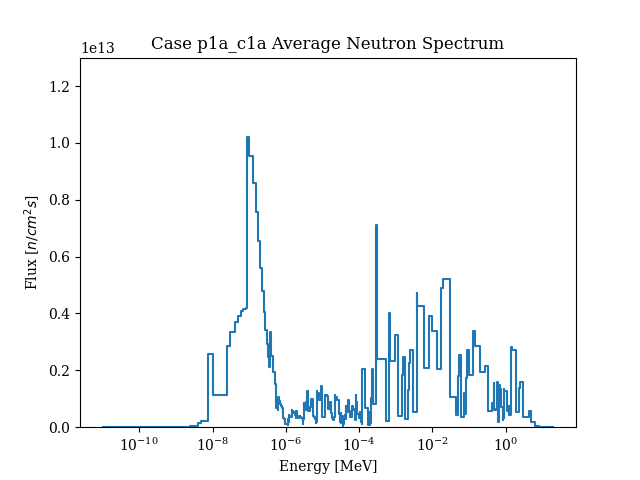
\includegraphics[width=0.75\linewidth]{p1a_c1a_f.png} 
    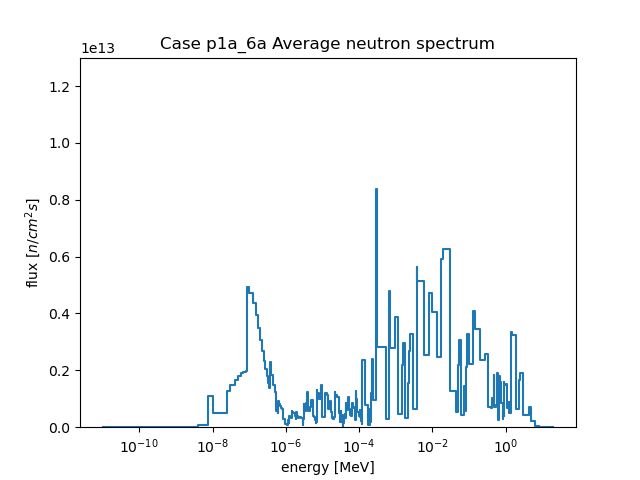
\includegraphics[width=0.75\linewidth]{p1a_c6a_f.png} 
    \caption{Neutron spectrum for \acrlong{FHR} Benchmark's Phase I-A Case 1A 
    (left) and Case 6A (right).}
    \label{fig:phase1a-f}
\end{figure}
Case 7A has a similar neutron spectrum as Case 6A since both cases have 
higher fuel content. 
All other cases have a similar neutron spectrum to Case 1A.
The neutron spectrum is faster for Cases 6A and 7A due to more heavy metal 
loading and higher enrichment, respectively.  

\subsection{Results: Phase I-B}
Figure \ref{fig:phase1b_keff} shows the $k_{eff}$ evolution during depletion 
for Cases 1B, 4B, and 7B.
\begin{figure}[]
    \centering
    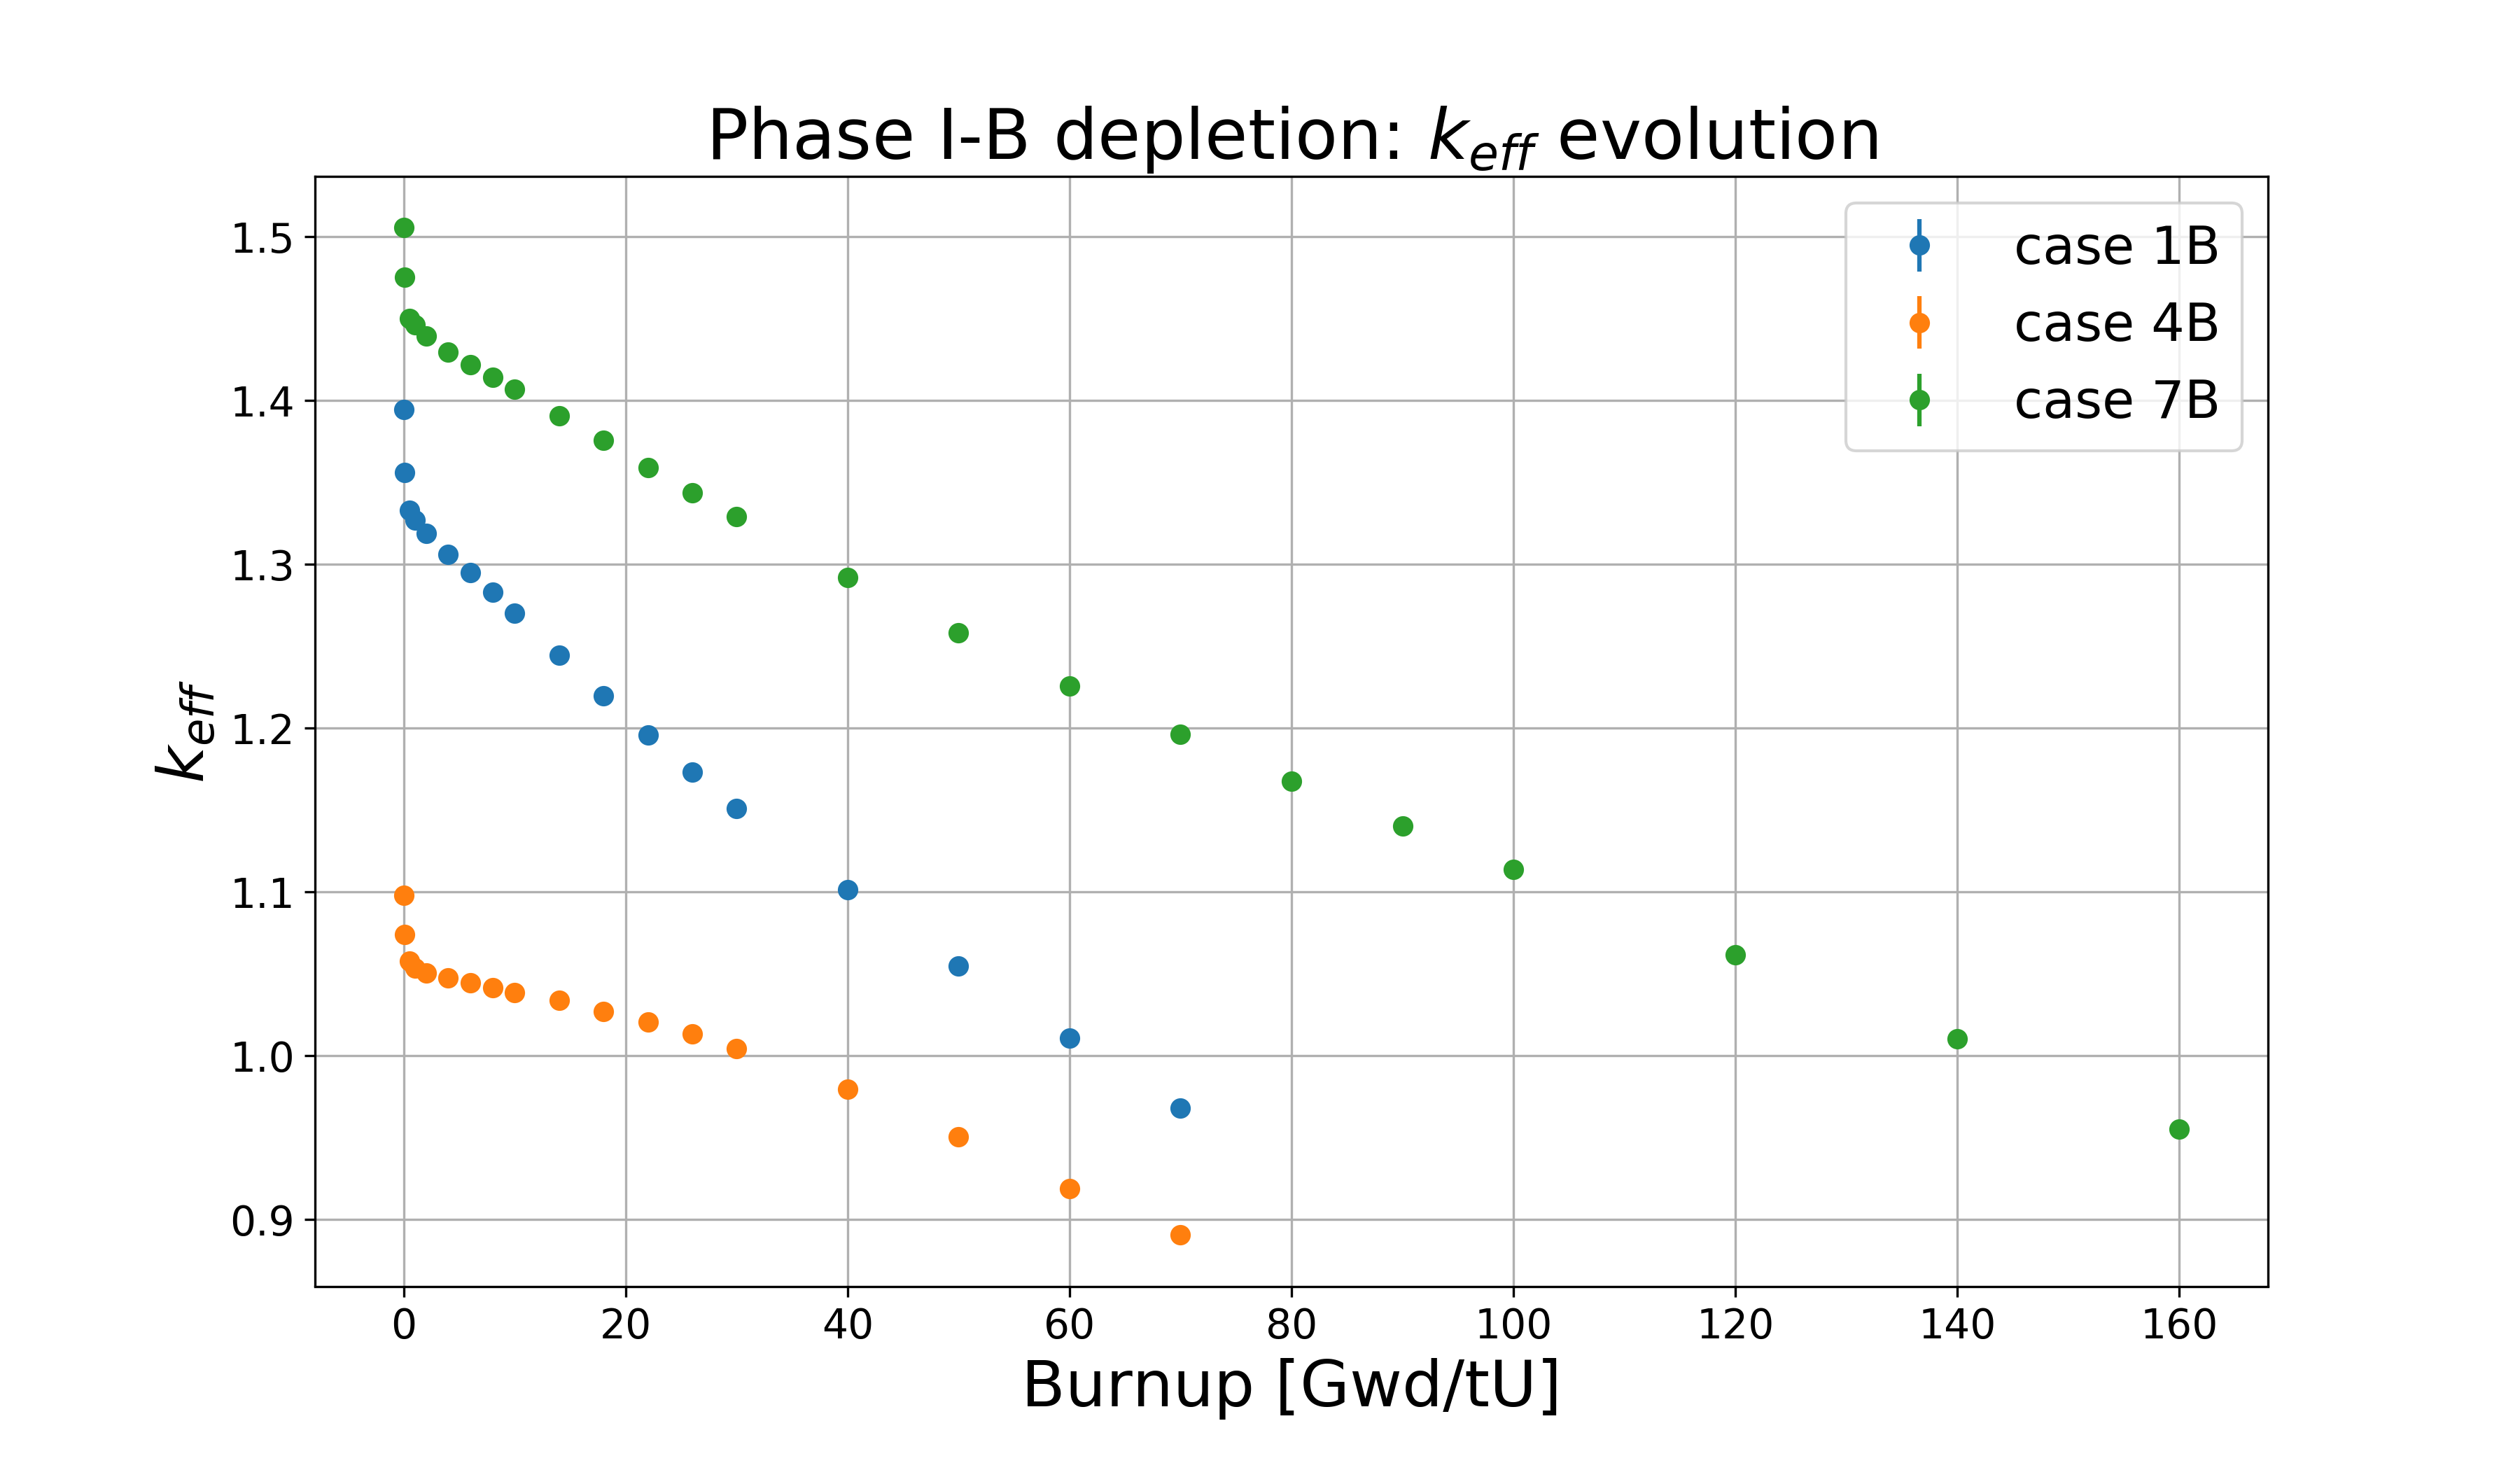
\includegraphics[width=1.1\linewidth]{phase1b_keff.png} 
    \caption{\acrlong{FHR} Benchmark's Phase I-B depletion $k_{eff}$ evolution 
    for Cases 1B, 4B, and 7B. Case 1B is the reference case, Case 4B is the 
    discrete \gls{BP} case, and Case 7B is the 19.75$\%$ enrichment case. 
    Error bars are included but are barely visible due to the low uncertainty 
    of $\sim$40pcm.}
    \label{fig:phase1b_keff}
\end{figure}
The $k_{eff}$ at zero burnup corresponds to each case's 
corresponding Phase I-A $k_{eff}$ value reported in Table \ref{tab:phase1a-results}. 
Case 1B is the reference case with $9\%$ fuel enrichment and no \glspl{BP}. 
Case 1B's $k_{eff}$ steadily decreases until it reaches 0.967845 at the final 70 
GWd/tU burnup. 
Case 4B includes burnable poisons resulting in a lower initial $k_{eff}$. 
Its $k_{eff}$ decreases at a slower rate in the beginning due to the presence of 
burnable poisons, which decreases flux in the core. 
At approximately 20 GWd/tU, $k_{eff}$ begins decreasing at a faster rate, assumedly
due to burn-up of the poison material.   
Case 7B has a $19.75\%$ fuel enrichment, resulting in a higher initial $k_{eff}$. 
With a higher enrichment, the fuel can achieve a final burnup of 160 GWd/tU. 

\section{Summary}
% more enrichment / more HM does not mean higher keff, there is shielding 
% effects, thus, this leads us to believe that the phenomena is not as expected. 

This chapter described the \gls{FHR} benchmark specifications, \gls{AHTR} design,
and Phase I-A and I-B results obtained by the UIUC team. 
The benchmark results highlight the \gls{AHTR}'s passive safety behavior with 
negative temperature coefficients. 
Results such as a lower $k_{eff}$ for the \gls{AHTR} configuration with 
higher heavy metal loading demonstrated how increased fuel packing does not always 
correspond with increased $k_{eff}$ due to self-shielding effects.
These results hint at the possibility of minimizing fuel required by optimizing 
for inhomogeneous fuel distributions within the core. 
This will be further explored in the later chapters. 


%\chapter{REALM: Reactor Evolutionary Algorithm Optimizer}
% Main Gist 
% - Genetic Algorithms / DEAP have been applied to a multitude of problems, 
%   but barely to nuclear. DEAP was created to be easily coupled with other
%   codes and to flexibly build your own reactor. 
% Structure 
% - Realm framework
% - Coupling to OpenMC and Moltres
\label{chap:realm}
In this chapter, I introduce the \gls{REALM} framework developed for the
proposed work.
\gls{REALM} is a Python package that applies evolutionary algorithm 
optimization techniques to nuclear reactor design. 
Applying evolutionary algorithms to nuclear design problems is not new, as I
previously discussed in Section \ref{sec:opt}, and available evolutionary algorithm 
packages can be customized for reactor design optimization problems. 
However, evolutionary algorithm setup is highly customizable with
an assortment of genetic algorithm designs and operators.
A reactor designer unfamiliar with evolutionary algorithms will have
to go through the cumbersome process of customizing a genetic algorithm 
for their needs and determine which operators and hyperparameters work best for 
their problem. 
Furthermore, computing fitness values with nuclear software is computationally 
expensive, necessitating using supercomputers and setting up parallelization 
for the genetic algorithm.

Therefore, the motivation behind creating REALM is to limit these inconveniences and 
facilitate using evolutionary algorithms for reactor design optimization.
\gls{REALM} provides a general genetic algorithm framework, sets up 
parallelization for the user, and promotes usability with an input file 
that only exposes mandatory parameters.
REALM also strives to be effective, flexible, open-source, parallel, reproducible, 
and usable. 
I briefly summarize how \gls{REALM} achieves these goals:  
\begin{itemize}
    \item Effective: \gls{REALM} is well documented, tested, and 
    version-controlled on Github \cite{chee_arfcrealm_2021}.
    \item Flexible: The proposed work aims to utilize \gls{REALM} to 
    explore arbitrary reactor geometries and inhomogeneous fuel distributions. 
    However, future users might want to utilize \gls{REALM} 
    to explore other arbitrary design parameters. Thus, I designed the \gls{REALM}
    framework accordingly. The user can vary any imaginable parameter 
    because \gls{REALM} uses a templating method to edit the input file of the 
    coupled software.
    \item Open-source: \gls{REALM} utilizes a well-documented, open-source 
    evolutionary algorithm Python package to drive the optimization process, 
    and established open-source nuclear software (OpenMC \cite{romano_openmc_2013} and 
    Moltres \cite{lindsay_introduction_2018}) to compute the objective function 
    and constraints. I also provide a simple tutorial for future developers to 
    follow for coupling other nuclear software to \gls{REALM}.  
    \item Parallel: \gls{REALM} runs in parallel on \gls{HPC} machines using the 
    \texttt{mpi4py} Python package \cite{dalcin_mpi_2008}.
    \item Reproducible: Data from every REALM run saves into a unique, pickled 
    file (pickle is a Python module that serializes Python objects), and all 
    results from this work are available on Github. 
\end{itemize}

\gls{REALM} essentially couples an evolutionary algorithm driver with nuclear 
software, such as neutron transport and thermal-hydraulics codes. 
Figure \ref{fig:genetic_alg} from Chapter \ref{chap:lit-review} outlines the 
evolutionary algorithm iterative problem solving process. 
I modified Figure \ref{fig:genetic_alg} to produce Figure 
\ref{fig:genetic_alg_nuclear}, which depicts how the nuclear transport and 
thermal-hydraulics software fit within the process. 
\begin{figure}[]
    \centering
    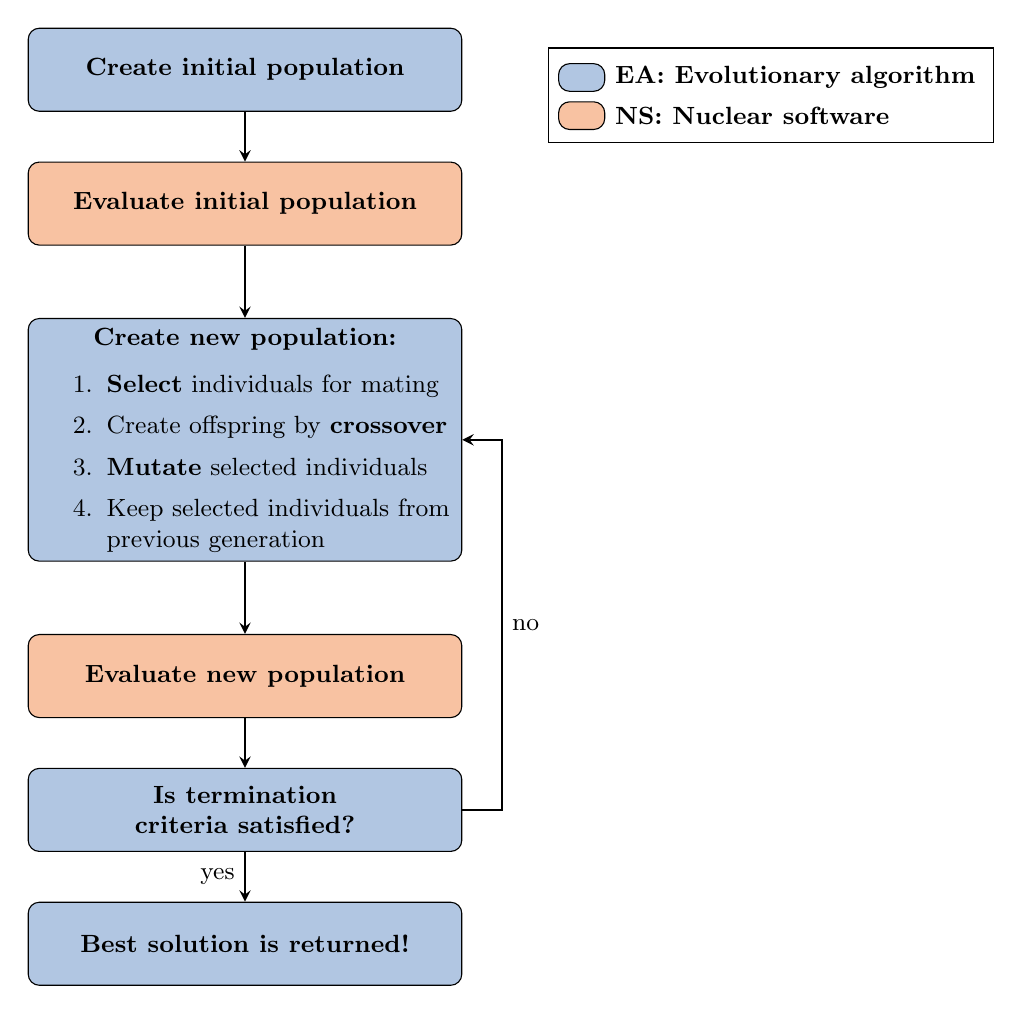
\begin{tikzpicture}[node distance=1.7cm]
            \tikzstyle{every node}=[font=\small]
            \node (1) [lbblock] {\textbf{Create initial population}};
            \node (2) [loblock, below of=1] {\textbf{Evaluate initial population}};
            \node (3) [lbblock, below of=2, yshift = -1.3cm] {\textbf{Create new population:} \\ 
            \begin{enumerate} \item \textbf{Select} individuals for mating 
                              \item Create offspring by \textbf{crossover} 
                              \item \textbf{Mutate} selected individuals 
                              \item Keep selected individuals from previous generation
                             \end{enumerate}};
            \node (4) [loblock, below of=3, yshift=-1.3cm] {\textbf{Evaluate new population}};
            \node (5) [lbblock, below of=4] {\textbf{Is termination \\ criteria satisfied?}};
            \node (6) [lbblock, below of=5] {\textbf{Best solution is returned!}};
            \draw [arrow] (1) -- (2);
            \draw [arrow] (2) -- (3);
            \draw [arrow] (3) -- (4);
            \draw [arrow] (4) -- (5);
            \draw [arrow] (5) -- node[anchor=east] {yes} (6);
            \draw [arrow] (5) -- ([shift={(0.5cm,0cm)}]5.east)-- node[anchor=west] {no} ([shift={(0.5cm,0cm)}]3.east)--(3);
            \matrix [draw,above right,yshift=10.7cm, xshift=0cm] at (current bounding box.south east) {
            \node [bbblock,label=right:\textbf{EA: Evolutionary algorithm}] {}; \\
            \node [boblock,label=right:\textbf{NS: Nuclear software}] {}; \\
            };
    \end{tikzpicture}
    \caption{Process of finding optimal solutions for a problem with a 
    genetic algorithm. Nuclear software evaluates each new population.}
    \label{fig:genetic_alg_nuclear}
\end{figure}
Therefore, \gls{REALM} initially reads and validates the JSON input 
file, initializes the \gls{DEAP} \cite{fortin_deap_2012} genetic algorithm 
hyperparameters and operators, and finally runs the genetic algorithm following 
the flow chart in Figure \ref{fig:genetic_alg_nuclear}, in which the nuclear 
software evaluates each individual's fitness. 

In the subsequent sections, I describe the evolutionary algorithm software (DEAP)
that drives \gls{REALM}, the nuclear software coupled to REALM, and details about 
the \gls{REALM} framework, such as the input file format and software architecture. 

\section{Evolutionary Algorithm Driver}
Evolutionary algorithm computation uses sophisticated, diverse techniques 
and mechanisms, resulting in even the most well-designed, software frameworks 
being complicated under the hood. 
Utilizing an existing evolutionary algorithm framework brings 
up issues in extending implementation intricacies as the user has to edit the 
source code \cite{fortin_deap_2012}. 
Therefore, an evolutionary algorithm computation framework that gives the user the 
capability to build custom evolutionary algorithms is ideal for this project.

There are many evolutionary algorithm computation packages available: 
\gls{DEAP} \cite{fortin_deap_2012}, inspyred \cite{garrett_inspyred_2014}, 
Pyevolve \cite{perone_pyevolve_2009}, and OpenBEAGLE \cite{gagne_open_2002}.
\gls{DEAP} is the newest package and places a high value on code 
compactness and clarity \cite{fortin_deap_2012}. 
\gls{DEAP} is the only framework that allows the user to prototype evolutionary 
algorithms rapidly and define custom algorithms without digging deep into 
the source code to modify lines.
This makes \gls{DEAP} the code of choice for the REALM framework's evolutionary 
algorithm driver component. 
\gls{DEAP} provides building blocks for each optimizer function and allows the 
user to customize a specialized algorithm to fit their project \cite{fortin_deap_2012}.

\subsection{\acrlong{DEAP}}
\label{sec:deap-works}
\gls{DEAP} is composed of two simples structures: a \textit{creator} and a 
\textit{toolbox}.  
The \textit{creator} module is a meta-factory that allows the run-time creation 
of classes via inheritance and composition, enabling individual and population 
creation from  from any data structure: lists, sets, dictionaries, trees, 
etc \cite{fortin_deap_2012}. 
The \textit{toolbox} is a container that the user manually populates.
In the \textit{toolbox}, the user defines the selection, crossover, and 
mutation operator types and hyperparameters. 
For example, the user registers a crossover operator under the `mate'
alias, and a selection operator under the `select' alias. 
Then, the evolutionary algorithm uses these aliased operators from the 
\textit{toolbox}. 
If the user wants to change the crossover operator, they would update the 
`mate' alias in the \textit{toolbox}, while keeping the evolutionary algorithm 
unchanged \cite{fortin_deap_2012}. 

Figure \ref{fig:deap-code} illustrates DEAP's usage of the \textit{creator} and
\textit{toolbox} modules. 
\begin{figure}[]
    \begin{minted}[
        frame=lines,
        framesep=2mm,
        baselinestretch=1.2,
        fontsize=\footnotesize,
        linenos
        ]{python}
        
        from deap import creator, base, tools, algorithms
        creator.create("Objective", base.Fitness, weights=(-1.0,)) # minimum
        creator.create("Individual", list, fitness=creator.Objective)

        toolbox = base.Toolbox()
        toolbox.register("variable_1", random.uniform, 0.0, 10.0)
        toolbox.register("variable_2", random.uniform, -1.0, 0.0)
        def individual_creator():
            return creator.Individual([toolbox.variable_1(), toolbox.variable_2()])
        toolbox.register("individual", individual_creator())
        toolbox.register("population", tools.initRepeat, list, toolbox.individual)
        def evaluator_fn(individual):
            return tuple([sum(individual)])
        toolbox.register("evaluate", evaluator_fn)
        toolbox.register("select", tools.selBest, k=5)
        toolbox.register("mutate", tools.mutPolynomialBounded, eta=0.5, low=[0, -1], up=[-1, 0])
        toolbox.register("mate", tools.cxOnePoint)
    \end{minted}
    \caption{DEAP sample code demonstrating the usage of the \textit{creator} and
    \textit{toolbox} modules to initialize the genetic algorithm. In REALM, DEAP's 
    \textit{creator} and \textit{toolbox} modules are initialized in the source 
    code based on the genetic algorithm parameters defined by the user in the 
    REALM input file. }
    \label{fig:deap-code}
\end{figure}
Line 2 creates a single-objective fitness class, \texttt{Objective}. 
The first argument defines the name of the derived class, the second argument 
specifies the inherited base class, \texttt{base.fitness}, and the third 
argument indicates the objective fitness ($-1.0$ indicates a minimum objective, 
$+1.0$ indicates a maximum objective). 
Line 3 derives an \texttt{Individual} class from the standard Python list type,
and defines its fitness attribute to be the newly created \texttt{Objective} object. 
Lines 5-9 initialize the \gls{DEAP} toolbox, register 
\texttt{variable\_1} and \texttt{variable\_2} with their upper and lower bounds, 
and define the \texttt{individual\_creator} function to return an 
\texttt{Individual} initialized with \texttt{variable\_1}, and \texttt{variable\_2}. 
Lines 10-11 and 14-17 are aliases for initializing individuals and population, 
specifying variation operators (\texttt{select}, \texttt{mutate}, \texttt{mate}), 
and evaluating individual fitness (\texttt{evaluate}) \cite{fortin_deap_2012}. 
Lines 12-13 define the evaluation function that returns the fitness values. 

In REALM, DEAP's \textit{creator} and \textit{toolbox} modules are initialized 
in the source code based on the genetic algorithm parameters defined by the user 
in the REALM input file. 
The evaluation function runs the nuclear software and returns user-defined 
fitness values. 

\subsection{General Genetic Algorithm Framework}
The creators' of DEAP provided variations of a classical genetic algorithm 
exposing different explicitness levels \cite{fortin_deap_2012}. 
The high-level examples use the in-built DEAP genetic algorithms, 
whereas the low-level example completely unpacks the genetic algorithm to expose 
a generational loop. 
The general genetic algorithm included in the \textbf{\textit{Algorithm}} class 
is based on the low-level example. 
The algorithm begins by initializing the starting population and evaluating 
each individual's fitness value. 
Then, it enters a generational loop. 
During each iteration, selection, mating, and mutation operators are applied to 
the population, then, the new individuals are evaluated, the constraints are 
applied, and the results are saved.

% include code here? 

\section{Nuclear Software}
Many nuclear software have restricted public access. 
In the proposed work, I enabled \gls{REALM} to work with open-source nuclear 
transport and thermal-hydraulics software, OpenMC \cite{romano_openmc_2013} 
and Moltres \cite{lindsay_introduction_2018}.  
OpenMC is an open-source Monte Carlo neutron transport code capable of 
performing k-eigenvalue calculations on models built using either constructive 
solid geometry or CAD representation. 
OpenMC can run in parallel using a hybrid \gls{MPI} and OpenMP programming model. 
Moltres is an open-source tool designed to simulate \glspl{MSR} using 
deterministic neutronics and thermal-hydraulics implemented as an application 
atop the \gls{MOOSE} finite-element framework.  
Moltres solves arbitrary-group neutron diffusion, temperature, and precursor 
governing equations on a single mesh and can be deployed on an arbitrary number 
of processing units \cite{lindsay_introduction_2018}.

OpenMC and Moltres are both open-source, well-documented, well-supported, and 
Github version-controlled codes that can run in parallel on \gls{HPC} machines.
Thus they achieve the \gls{REALM} goals listed at the start of this chapter, 
making them suitable to be used as \gls{REALM}'s nuclear software.
However, users can easily use restricted nuclear software with \gls{REALM} 
by coupling \gls{REALM} with the restricted software on their local machine. 
In the REALM documentation \cite{chee_arfcrealm_2021}, I outline how to couple 
other nuclear software to REALM. 

\section{REALM Input File}
REALM's input file is in JSON format. 
There are four sections that the user must define: \\ \texttt{control\_variables}, 
\texttt{evaluators}, \texttt{constraints}, and \texttt{algorithm}. 
Figure \ref{fig:realm-input} shows an example REALM input file. 
In this simulation, REALM uses a genetic algorithm with the defined 
hyperparameters to minimize the \texttt{output1} parameter which is 
calculated using the OpenMC evaluator that accepts input parameters: 
\texttt{variable1} and \texttt{variable2}. 
\begin{figure}[]
    \begin{minted}[
        frame=lines,
        framesep=2mm,
        baselinestretch=1.2,
        fontsize=\footnotesize,
        linenos
        ]{json}
        {
            "control_variables": {
                "variable1": {"min": 0.0, "max": 10.0}, 
                "variable2": {"min": -1.0, "max": 0.0}
            }, 
            "evaluators": {
                "openmc": {
                    "input_script": "openmc_inp.py",
                    "output_script": "openmc_output.py", 
                    "inputs": ["variable1", "variable2"],
                    "outputs": ["output1", "output2"]
                }
            }, 
            "constraints": {
                "output1": {"operator": [">=", "<"], "constrained_val": [1.0, 1.5]}
            }, 
            "algorithm": {
                "objective": "min", 
                "optimized_variable": "output1", 
                "pop_size": 100, 
                "generations": 10, 
                "mutation_probability": 0.5,
                "mating_probability": 0.5,
                "selection_operator": {"operator": "selBest", "k": 1},
                "mutation_operator": {
                    "operator": "mutPolynomialBounded",
                    "indpb": 0.5,
                    "eta": 0.5
                },
                "mating_operator": {"operator": "cxOnePoint"}
            }
        }
    \end{minted}
    \caption{\acrfull{REALM} sample JSON input file.}
    \label{fig:realm-input}
\end{figure}

Next, I will describe how to define each section of a REALM input file. 
The \gls{REALM} documentation \cite{chee_arfcrealm_2021} provides further 
descriptions for setting up a \gls{REALM} input file.

\subsection{Control Variables}
Control variables are parameters the genetic algorithm will vary. 
For each control variable, the user must specify its minimum and maximum values.
For example, Lines 2 to 5 in Figure \ref{fig:realm-input} demonstrate that the 
control variables, \texttt{variable1} and \texttt{variable2}, 
will be varied from 0 to 10 and -1 to 0, respectively. 

\subsection{Evaluators}
Evaluators are the nuclear software REALM utilizes to calculate objective functions. 
Presently, only \texttt{openmc} and \texttt{moltres} evaluators are available 
in REALM.
In a single REALM input file, a user may define any number of evaluators. 
For each evaluator, mandatory input parameters are \texttt{input\_script}, 
\texttt{inputs}, and \texttt{outputs}, and the optional input parameter is
\texttt{output\_script}. 
The \texttt{input\_script} is input file template's name for the evaluator software. 
The user must include a input file template in the same directory as the REALM input 
file. 
The \texttt{inputs} parameter lists the control variables that are placed into the 
input file template. 
REALM utilizes jinja2 templating to insert the control variable values into the 
\texttt{input\_script}. 
Lines 6 to 12 in the REALM input file (Figure \ref{fig:realm-input}) demonstrate 
that \texttt{variable1} and \texttt{variable2} are \texttt{inputs} into the 
\texttt{openmc\_inp.py} \texttt{input\_script}. 
Figure \ref{fig:openmcinp.py} shows the template and templated openmc script; 
once the \texttt{openmc\_inp.py} \texttt{input\_script} is templated, 
\texttt{\{\{variable1\}\}} and \texttt{\{\{variable2\}\}}  on Lines 3 and 4 will be 
replaced with values selected by the REALM genetic algorithm. 
\begin{figure}[]
    \begin{minipage}{0.4\textwidth}
        \centering
    \begin{minted}[
        frame=lines,
        framesep=2mm,
        baselinestretch=1.2,
        fontsize=\footnotesize,
        linenos
        ]{python}
        import openmc 
        # templating 
        variable1 = {{variable1}}
        variable2 = {{variable2}}
        # run openmc 
        ... 
    \end{minted}
    \end{minipage}
    \hspace{2cm}
    \begin{minipage}{0.4\textwidth}
        \centering
        \begin{minted}[
            frame=lines,
            framesep=2mm,
            baselinestretch=1.2,
            fontsize=\footnotesize,
            linenos
            ]{python}
            import openmc 
            # templating 
            variable1 = 3.212
            variable2 = -0.765
            # run openmc 
            ... 
        \end{minted}
        \end{minipage}
    \caption{\texttt{openmc\_inp.py} input script template (left). 
             Templated \texttt{openmc\_inp.py} with variable1 and variable2 
             values defined (right).}
    \label{fig:openmcinp.py}
\end{figure}

The \texttt{outputs} parameter lists the output variables that the evaluator 
will return to the genetic algorithm. 
These output parameters are also known as the objective functions used to 
evaluate the individual.  
\gls{REALM} uses three methods to return an output parameter. 
First, if the output parameter is also an input parameter, REALM will automatically 
return the input parameter's value. 
Second, the user can use predefined evaluations. 
For example, in \texttt{OpenMCEvaluation}, there is a predefined $k_{eff}$ 
evaluation.
The user may also add predefined evaluations to \texttt{OpenMCEvaluation} or 
\texttt{MoltresEvaluation}, or any other coupled codes' evaluation file.
Third, the user may include an \texttt{output\_script} that returns the desired 
output parameters. 
The \texttt{output\_script} must include a line that prints a dictionary containing 
the output parameters' names and their corresponding value as key-value pairs. 

\subsection{Constraints}
In the constraints section, the user can define constraints on any output parameter. 
Any individual that does not meet the defined constraints is removed from the 
population, encouraging the proliferation of individuals that meet the 
constraints. 
For each constrained output parameter, the user lists the \texttt{operator}s 
and \texttt{constrained\_val}s as in Line 15 of the REALM input file 
(Figure \ref{fig:realm-input}). 
Thus, for this REALM simulation, \texttt{output\_1} is constrained to be 
$>= 1.0$ and $< 1.5$. 

\subsection{Algorithm}
%Selection Operator: Tournament selection Selection pressure, a probabilistic 
%measure of a chromosome's likelihood of participation in the tournament based 
%on the participant selection pool size, is easily adjusted by changing the 
%tournament size, the reason is that if the tournament size is larger, weak 
%individuals have a smaller chance to be selected, because, if a weak 
%individual is selected to be in a tournament, there is a higher probability 
%that a stronger individual is also in that tournament.

In the algorithm section, the user defines all the hyperparameters for the 
genetic algorithm. 
The mandatory input parameters include \texttt{optimized\_variable}, 
\texttt{objective}, \texttt{pop\_size}, and \texttt{generations}.
The user specifies an \texttt{optimized\_variable}, which must be an output 
parameter from the evaluators' \texttt{outputs}. 
The user has the option to maximize or minimize this \texttt{optimized\_variable}
by defining the \texttt{objective} variable as \texttt{max} or \texttt{min}. 
The user must also specify the population size (\texttt{pop\_size}) and number 
of generations (\texttt{generations}) in the genetic algorithm. 

The optional input parameters include \texttt{mutation\_probability}, 
\texttt{mating\_probability}, \\ \texttt{selection\_operator}, 
\texttt{mutation\_operator}, and \texttt{mating\_operator}. 
As mentioned previously in Section \ref{sec:genetic_alg}, it is important to 
select genetic algorithm hyperparameters that balance the extent of exploration 
and exploitation.
The user can define the mutation and mating probability or not define them which 
results in the default values of 0.3 and 0.4, respectively. 
For each operator, the user can choose from a list of operators and define each
of their required hyperparameters. 
Table \ref{tab:deap_operators} shows the available operators and their respective 
hyperparameters. 
\begin{table}[]
    \centering
    \onehalfspacing
    \caption{Selection, mutation, and mating operators available in 
    \acrfull{REALM} and their corresponding hyperparameters. }
	\label{tab:deap_operators}
    \footnotesize
    \begin{tabular}{l|p{0.23\textwidth}|p{0.55\textwidth}}
    \hline
    \textbf{Operator} & \textbf{Available Options} & \textbf{Hyperparameters} \\ \hline
    \multirow{4}{1cm}{Selection} & \multirow{2}{2cm}{\texttt{selTournament}} & \texttt{tournsize}: no. of individuals in each tournament\\ 
    & & \texttt{k}: no. of individuals to select \\ \cline{2-3}
    & \texttt{selNSGA2} & \texttt{k}: no. of individuals to select\\ \cline{2-3}
    & \texttt{selBest} & \texttt{k}: no. of individuals to select\\ \hline
    \multirow{2}{1cm}{Mutation} & \multirow{2}{2cm}{\texttt{mutPolynomialBounded}} & \texttt{eta}: crowding degree of the mutation\\  
    && \texttt{indpb}: independent probability for each attribute to be mutated\\ \hline
    \multirow{3}{1cm}{Mating} & \texttt{cxOnePoint} & -\\ \cline{2-3}
    & \texttt{cxUniform} & \texttt{indpb}: independent probability for each attribute to be exchanged\\ \cline{2-3}
    & \texttt{cxBlend} & \texttt{alpha}: Extent of the interval in which the new values can be drawn for each attribute on both side of the parents’ attributes\\ \hline
    \end{tabular}
    \end{table}
% fill this out properly later. 
The default selection operator is \texttt{selNSGA2} with a default
\texttt{k} value, two-thirds the population size. 
The default mutation operator is \texttt{mutPolynomialBounded} with default
\texttt{eta} and \texttt{indpb} values of 0.3. 
The default mating operator is \texttt{cxBlend} with a default \texttt{alpha} 
of 0.4. 
Lines 17 to 31 in the example REALM input file (Figure \ref{fig:realm-input}) 
demonstrate \texttt{algorithm} specifications. 

\section{REALM Software Architecture}
In this section, I will describe \gls{REALM} v1.0's software architecture and 
how all the parts come together to optimize reactor design. 
Table \ref{tab:realm-architecture} outlines the classes in the REALM software 
and describes each class's purpose.
\begin{table}[]
    \centering
    \onehalfspacing
    \caption{Classes that makeup REALM's architecture and their description. }
	\label{tab:realm-architecture}
    \footnotesize
    \begin{tabular}{l|p{0.73\textwidth}}
    \hline
    \textbf{Class} & \textbf{Description} \\ \hline
    \textbf{\textit{InputValidation}} & The \textbf{\textit{InputValidation}} class contains methods 
    to read and validate the JSON \gls{REALM} input file to 
    ensure the user defined all key parameters. If they did not, \gls{REALM} 
    raises an exception to tell the user which parameters are missing. \\
    \hline
    \textbf{\textit{Evaluation}} & \gls{DEAP}'s fitness evaluator (as mentioned in Section 
    \ref{sec:deap-works}) requires an evaluation function to evaluate each 
    individual's fitness values. 
    The \textbf{\textit{Evaluation}} class contains a method that creates an evaluation 
    function that runs the nuclear software and returns the required fitness values, 
    defined in the input file. \\
    \hline 
    \textbf{\textit{OpenMCEvaluation}} & The \textbf{\textit{OpenMCEvaluation}} class contains
    built-in methods for evaluating OpenMC output files. Developers can update 
    this file with methods to evaluate frequently used OpenMC outputs. \\
    \hline 
    \textbf{\textit{ToolboxGenerator}} & The \textbf{\textit{ToolboxGenerator}} class initializes
    DEAP's \textit{toolbox} and \textit{creator} modules with genetic algorithm 
    hyperparameters defined in the input file.\\
    \hline
    \textbf{\textit{Constraints}} & The \textbf{\textit{Constraints}} class 
    contains methods to initialize constraints defined in the input file 
    and applies the constraints by removing individuals that do not meet the 
    constraint.\\
    \hline 
    \textbf{\textit{BackEnd}} & The \textbf{\textit{BackEnd}} class contains methods to save 
    genetic algorithm population results into a pickled checkpoint file and to 
    restart a partially completed genetic algorithm from the checkpoint file. \\
    \hline
    \textbf{\textit{Algorithm}} & The \textbf{\textit{Algorithm}} class contains methods to 
    initialize and execute the genetic algorithm. It executes a general genetic 
    algorithm framework that uses the hyperparameters defined in the 
    \textbf{\textit{ToolboxGenerator}}, applies constraints defined in
    \textbf{\textit{Constraints}}, evaluates fitness values using the evaluation 
    function produced by \textbf{\textit{Evaluation}}, and saves all the results 
    with \textbf{\textit{BackEnd}}. \\
    \hline
    \textbf{\textit{Executor}} & The \textbf{\textit{Executor}} class drives the \gls{REALM} code
    execution with the following steps: \\
    & 1) User input file validation with \textbf{\textit{InputValidation}} \\
    & 2) Evaluation function generation with \textbf{\textit{Evaluation}} \\
    & 3) DEAP toolbox initialization with \textbf{\textit{ToolboxGenerator}} \\ 
    & 4) Constraint initialization with \textbf{\textit{Constraints}} \\ 
    & 5) Genetic algorithm execution with \textbf{\textit{Algorithm}} \\
    \hline
    \end{tabular}
    \end{table}
Figure \ref{fig:realm_archi} depicts REALM's software architecture. 
\begin{figure}[]
    \centering
    \begin{tikzpicture}[node distance=0.5cm]
        \tikzstyle{every node}=[font=\footnotesize]
        \node (1) [b72block] {\textbf{\textit{InputValidation}}};
        \node (2) [b72block, below=of 1] {\textbf{\textit{Evaluation}}};
        \node (9) [b82block, left=of 2, yshift=0.5cm] {\textbf{\textit{OpenMCEvaluation}}};
        \node (3) [b72block, below=of 2] {\textbf{\textit{ToolboxGenerator}}};
        \node (10) [b82block, left=of 3, yshift=0.5cm] {\textbf{\textit{MoltresEvaluation}}};
        \node (4) [b72block, below=of 3] {\textbf{\textit{Constraints}}};
        \node (5) [b72block, below=of 4] {\textbf{\textit{BackEnd}}};
        \node (6) [b223block, right=of 2, yshift=0cm, xshift=0.6cm] 
        {\baselineskip=14.5pt \textbf{\textit{Executor}} \\ \raggedright 
        1) User input file validation with \textbf{\textit{InputValidation}} \\ 
        2) Evaluation function generation with \textbf{\textit{Evaluation}} \\ 
        3) DEAP toolbox initialization with \textbf{\textit{ToolboxGenerator}} \\ 
        4) Constraints initialization with \textbf{\textit{Constraints}} \\ 
        5) Genetic algorithm execution with \textbf{\textit{Algorithm}} \\};
        \draw [arrow] (1) -- ([shift={(0cm,0cm)}]1.east) -- ([shift={(-0.5cm,0.8cm)}]6.west)--([shift={(0cm,0.8cm)}]6.west);
        \draw [arrow] (2) -- ([shift={(0cm,0cm)}]2.east) -- ([shift={(-0.5cm,0.3cm)}]6.west)--([shift={(0cm,0.3cm)}]6.west);
        \draw [arrow] (9) -- ([shift={(0cm,0cm)}]9.east) -- ([shift={(0cm,0cm)}]2.west);
        \draw [arrow] (10) -- ([shift={(0cm,0cm)}]10.east) -- ([shift={(0cm,0cm)}]2.west);
        \draw [arrow] (3) -- ([shift={(0cm,0cm)}]3.east) -- ([shift={(-0.5cm,-0.25cm)}]6.west)--([shift={(0cm,-0.25cm)}]6.west);
        \draw [arrow] (4) -- ([shift={(0cm,0cm)}]4.east) -- ([shift={(-0.5cm,-0.8cm)}]6.west)--([shift={(0cm,-0.8cm)}]6.west);
        \node (7) [b223block, right=of 4, yshift=-0.8cm, xshift=0.6cm] 
        {\baselineskip=14.5pt \textbf{\textit{Algorithm}} \\ \raggedright 
        1) Accepts initialized toolbox, constraints, and evaluator \\ \hspace{0.3cm} function \\
        2) Runs the genetic algorithm \\
        3) Saves results with \textbf{\textit{BackEnd}} \\};
        \draw [arrow] (7) -- ([shift={(0.cm,0.25cm)}]7.north) -| ([shift={(-0.5cm,-1.25cm)}]6.west) -- ([shift={(0cm,-1.25cm)}]6.west);
        \draw [arrow] (5) -- ([shift={(0cm,0cm)}]5.east) -- ([shift={(-0.5cm,-1cm)}]7.west)--([shift={(0cm,-1cm)}]7.west);
    \end{tikzpicture}
    \caption{Visualization of REALM architecture.}
    \label{fig:realm_archi}
\end{figure}
% how to run realm: python realm -i square.json -p max
When the user runs a REALM input file, the \textbf{\textit{Executor}} class 
drives REALM's execution from beginning to end.
The \textbf{\textit{Executor}} calls \textbf{\textit{InputValidation}} to 
parse the input file to ensure that the user defined all mandatory parameters
and used the correct formatting.
Next, it initializes an \textbf{\textit{Evaluator}} object based on the 
\texttt{evaluators} specifications in the input file. 
It uses the \textbf{\textit{Evaluator}} object to create a function that will 
run each evaluator software with the desired input parameters and return the 
output parameters calculated by the evaluator software. 
Next, it uses the \textbf{\textit{ToolboxGenerator}} to create an initialized 
DEAP toolbox object based on the input file's \texttt{algorithm} specifications. 
The \textbf{\textit{ToolboxGenerator}} object accepts the 
\textbf{\textit{Evaluator}} object and registers it as the toolbox's `evaluate' 
tool.  
Then, it initializes a \textbf{\textit{Constraints}} object to contain 
\texttt{constraints} specified in the input file. 
Next, the \textbf{\textit{Executor}} initializes an \textbf{\textit{Algorithm}} 
object that accepts the initialized DEAP toolbox and \textbf{\textit{Constraints}} 
object. 
Finally, the \textbf{\textit{Executor}} class uses a method in the 
\textbf{\textit{Algorithm}} object to run a general genetic algorithm with 
hyperparameters from the DEAP toolbox, apply constraints defined in the 
\textbf{\textit{Constraints}} object, and calculate objective functions using 
the evaluation function created by the \textbf{\textit{Evaluator}} object, all 
the while saving the results using the \textbf{\textit{BackEnd}} class. 

In the REALM Github repository \cite{chee_arfcrealm_2021}, I included a tests 
directory that contains unit tests for all methods in the classes described 
above. 

\subsection{Installing and Running REALM}
% python realm -i square.json -p max 
% checkpoint.pkl 
There are two ways to install REALM.
First, a user can utilize \gls{PyPI} to install REALM: \texttt{pip install realm}.
Second, a user can download the REALM Github repository \cite{chee_arfcrealm_2021}
and install it from source. 

REALM is run from the command line interface. 
A user should first set up the REALM JSON input file and evaluator 
scripts in a directory. 
When running REALM from the command line, there are two mandatory arguments and 
one optional argument. 
The mandatory arguments are the input file (\texttt{-i}) and objective (\texttt{-p}). 
The optional argument is the checkpoint file (\texttt{-c}).  
Thus, the structure of a command line input for running REALM is: 
\begin{verbatim}
    python realm -i <input file name> -p <max or min> -c <checkpoint file name>
\end{verbatim} 

The checkpoint file holds the results from the REALM simulation and also acts 
as a restart file. 
Thus, if a REALM simulation ends prematurely, the checkpoint file can be used 
to restart the code from the most recent population and continue the simulation. 

\subsection{REALM Results Analysis}
The \textbf{\textit{BackEnd}} class manages each REALM simulation's results. 
\textbf{\textit{BackEnd}} puts all the results in a pickled dictionary, and it 
is saved as \texttt{checkpoint.pkl} in the same directory as the input file. 
The checkpoint file can then be reloaded into a Jupyter notebook and organized 
to produce desired plots. 
Examples of REALM results analysis can be found in the REALM documentation 
\cite{chee_arfcrealm_2021}. 

The evaluation function creates a new directory for each software, generation, 
and individual and stores the templated input file and output files associated 
with that particular run. 
The generation and individual values are indexed by zero. 
For example, the directory containing files associated with an OpenMC run for 
the tenth individual in the genetic algorithm's third generation will be named: 
\texttt{openmc\_2\_9}.

%\subsection{Using REALM on a HPC}


%\section{Hyperparameter Search}
%Hyperparameters are a model configuration argument specified by the developer to 
%guide the learning process for a specific dataset. 

\section{Summary}
This chapter described the \acrfull{REALM} framework developed for the
proposed work. 
\gls{REALM} is a Python package that applies evolutionary algorithm 
optimization techniques to nuclear reactor design using the \acrfull{DEAP} 
module, OpenMC, and Moltres nuclear software. 
The motivation for REALM's inception is to enable reactor designers to utilize 
robust evolutionary algorithm optimization methods without going 
through the cumbersome process of setting up a genetic algorithm framework,
selecting appropriate hyperparameters, and setting up its parallelization. 
REALM is designed to be effective, flexible, open-source, parallel, 
reproducible, and usable and is hosted on Github \cite{chee_arfcrealm_2021}. 
%\chapter{REALM Demonstration}
% Main Gist 
% - Demonstrate OpenMC problem with REALM. 
% Structure 
% - realm demonstration of OpenMC Coupling for a toy problem. 
This chapter demonstrates using \gls{REALM} to apply genetic algorithms 
to maximize $k_{eff}$ in a single \gls{AHTR} fuel slab.  

\section{Straightened AHTR Fuel Slab}
\subsection{Problem Definition}
This demonstration explores how inhomogeneous fuel 
distributions impact $k_{eff}$ compared to homogenous fuel distributions that 
are customary in most reactor designs. 
The reactor core explored is a straightened slab from the \gls{FHR} benchmark's
\gls{AHTR} design.
Figure \ref{fig:straightened_slab} illustrates the straightened fuel slab. 
\begin{figure}[]
    \centering
    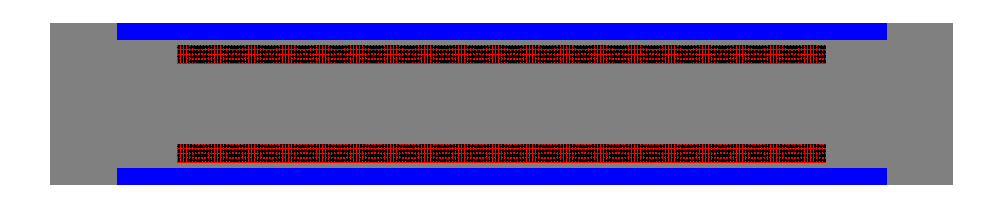
\includegraphics[width=\linewidth]{straightened_slab.png}
    \raggedright
    \resizebox{0.3\textwidth}{!}{
        \hspace{1cm}
        \fbox{\begin{tabular}{ll}
            \textcolor{fhrblue}{$\blacksquare$} & FLiBe \\
            \textcolor{fhrgrey}{$\blacksquare$} & Graphite (Fuel Plank)\\
            \textcolor{fhrred}{$\blacksquare$} & Graphite (Fuel Stripe) \\
            \textcolor{fhrblack}{$\blacksquare$} & TRISO particle 

            \end{tabular}}}
    \caption{Straightened \acrfull{AHTR} fuel slab.}
    \label{fig:straightened_slab}
\end{figure}
The slab has dimensions of $27.1 \times 3.25 \times 1.85\ cm^3$
with periodic boundary conditions in the x and y directions and reflective 
boundary conditions in the z-direction. 
The materials are the same as in the \gls{FHR} benchmark, except for 
the homogenization of each \gls{TRISO} particle's four outer layers: 
porous carbon buffer, inner pyrolytic carbon, silicon carbide layer, and the 
outer pyrolitic carbon. 
The \gls{TRISO} particles' dimensions remain the same.
The $k_{eff}$ for this original straightened \gls{AHTR} configuration is 
$1.38625 \pm 0.00109$. 

The \gls{REALM} optimization problem's objective is to maximize the slab's 
$k_{eff}$ by varying the \gls{TRISO} particle packing fraction across the slab
while keeping total \gls{TRISO} particle the total packing fraction constant at 
0.0979. 
This total packing fraction is consistent with the original straightened slab with 
TRISO particles in fuel stripes (Figure \ref{fig:straightened_slab}). 
The slab is divided into ten slices along the x-axis between the \gls{FLiBe} and 
graphite buffers resulting in ten $2.31 \times 2.55 \times 1.85\ cm^3$ slices. 
A sine distribution governs the \gls{TRISO} particle packing fraction's 
distribution across slices:
\begin{align}
    PF(x) &= (a\ sin(bx + c) + 2) \times NF\\
    \intertext{where}
    PF &= \mbox{packing fraction} \nonumber \\ 
    a &= \mbox{amplitude, peak deviation of the function from zero} \nonumber \\
    b &= \mbox{angular frequency, rate of change of the function argument } [\frac{radians}{s}] \nonumber \\
    c &= \mbox{phase, specifies (in radians) where in its cycle the oscillation is at t = 0.} \nonumber \\
    x &= \mbox{midpoint value for each slice} \nonumber \\
    NF &= \mbox{Normalization factor} \nonumber
\end{align}
The sine distribution's value at each of the ten x-slices' midpoints is collected 
and normalized by the total packing fraction to ensure a consistent amount of 
\gls{TRISO} particles in the slab.
Thus, for a packing fraction distribution of 
$PF(x) = (0.5\ sin(\frac{\pi}{3}x + \pi) + 2)  \times NF$. 
The packing fraction for the ten slices are 0.103, 0.120, 0.049, 0.138, 
0.076, 0.081, 0.136, 0.048, 0.125, 0.098, respectively. 
Figure \ref{fig:triso_distribution} shows a plot of this sine distribution, highlights 
the packing fraction at the respective midpoints, and an XY view of the slab
with packing fraction varying based on this sine distribution. 
\begin{figure}[]
    \centering
    \makebox[\textwidth][c]{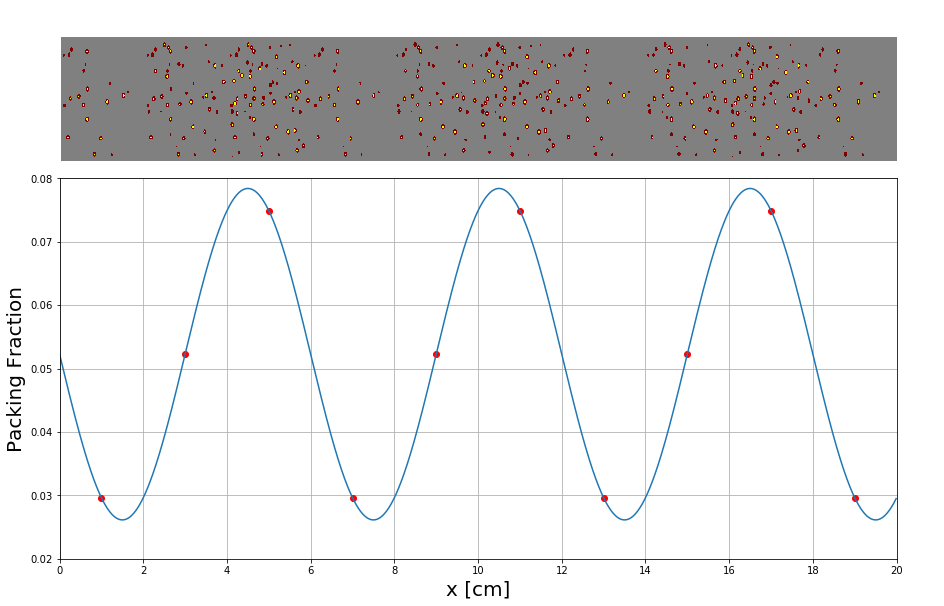
\includegraphics[width=1.1\linewidth]{triso_distribution_sine.png}} 
    \caption{Below: $PF(x) = (0.5\ sin(\frac{\pi}{3}x + \pi) + 2)  \times NF$ 
    sine distribution with red points indicating the packing fraction at each slice. 
    Above: Straightened \acrfull{AHTR} fuel slab with varying \gls{TRISO} particle 
    distribution across ten slices based on the sine distribution. }
    \label{fig:triso_distribution}
\end{figure}

In \gls{REALM}, a genetic algorithm varies the $a$, $b$, and $c$ variables to 
find a combination that produces a packing fraction distribution that maximizes 
the slab's $k_{eff}$. 
The upper and lower bounds of $a$, $b$ and $c$ are: 
\begin{itemize}
    \item 0 $<$ $a$ $<$ 2 
    \item 0 $<$ $b$ $<$ $\frac{\pi}{2}$
    \item 0 $<$ $c$ $<$ $2\pi$
\end{itemize}
The $a$ variable's bounds were selected to keep the sine distribution from falling 
below zero. $b$ and $c$ variable bounds are large enough to allow the genetic 
algorithm to explore various sine distributions. 
The OpenMC evaluator calculates $k_{eff}$. 
Each OpenMC simulation is run with 80 active cycles, 20 inactive cycles, and 
8000 particles to reach an uncertainty of approximately 130pcm. 
Figure \ref{fig:realm-input-simple} shows the \gls{REALM} input file for this 
genetic algorithm optimization problem. 
\texttt{ahtr\_slab\_openmc.py} is the template OpenMC straightened \gls{AHTR} 
slab script that accepts $a$, $b$ and $c$ from \gls{REALM}, calculates packing 
fraction distribution, and assigns packing fraction values to each fuel slice. 
Subsequently, \gls{REALM} runs the templated OpenMC script to generate $k_{eff}$. 
\begin{figure}[]
    \begin{minted}[
        frame=lines,
        framesep=2mm,
        baselinestretch=1.2,
        fontsize=\footnotesize,
        linenos
        ]{json}
        {
            "control_variables": {
                "a": {"min": 0.0, "max": 2.0},
                "b": {"min": 0.0, "max": 1.57},
                "c": {"min": 0.0, "max": 6.28},
            },
            "evaluators": {
                "openmc": {
                    "input_script": "ahtr_slab_openmc.py",
                    "inputs": ["a", "b", "c"],
                    "outputs": ["keff"],
                    "keep_files": false,
                }
            },
            "constraints": {"keff": {"operator": [">="], "constrained_val": [1.0]}},
            "algorithm": {
                "objective": "max",
                "optimized_variable": "keff",
                "pop_size": 60,
                "generations": 10,
                "mutation_probability": 0.23,
                "mating_probability": 0.46,
                "selection_operator": {"operator": "selTournament", "k": 15, "tournsize": 5},
                "mutation_operator": {
                    "operator": "mutPolynomialBounded",
                    "eta": 0.23,
                    "indpb": 0.23,
                },
                "mating_operator": {"operator": "cxBlend", "alpha": 0.46},
            },
        }
        
    \end{minted}
    \caption{\acrfull{REALM} JSON input file to maximize $k_{eff}$ in the 
    straightened \acrfull{AHTR} fuel slab by varying packing fraction distribution 
    with control variables, $a$, $b$, $c$.}
    \label{fig:realm-input-simple}
\end{figure}

\subsection{Hyperparameter Search}
In \gls{REALM}'s input file, the user can define the genetic algorithm's 
hyperparameters. 
A good hyperparameter set guides the optimization process by 
balancing exploitation and exploration to find an optimal solution quickly 
and accurately. 
Finding a good set of hyperparameters requires a trial and error process. 

I performed the hyperparameter search with a coarse-to-fine random sampling scheme, 
whose advantages were previously discussed in Section \ref{sec:balance}.
The hyperparameters varied include population size, number of generations, 
mutation probability, mating probability, selection operator, selection operator's 
number of individuals, selection operator's tournament size, mutation operator, 
and mating operator.  
I started with 25 coarse experiments and fine-tuned the hyperparameters
with 15 more experiments. 
For each genetic algorithm experiment, I hold the number of OpenMC evaluations 
constant at 600.
The number of evaluations correlates the population size and number of generations. 
I randomly sample population size and use the following equation to calculate 
the number of generations: 
\begin{align}
    \mbox{no. of generations} &= \frac{\mbox{no. of evaluations}}{\mbox{population size} }
\end{align}
Table \ref{tab:hyperparameter_search} shows the lower and upper bounds used 
for random sampling of each hyperparameter. 
\begin{table}[]
    \centering
    \onehalfspacing
    \caption{Hyperparameter search is conducted in three phases: \textit{Coarse Search}, 
    \textit{Fine Search 1}, \textit{Fine Search 2}. Each hyperparameter's lower and
    upper bounds for each phase of the search is listed.}
	\label{tab:hyperparameter_search}
    \footnotesize
    \makebox[\textwidth][c]{\begin{tabular}{p{4cm}lp{3.4cm}p{3.4cm}p{3.4cm}}
    \hline 
    \textbf{Hyperparameter}& \textbf{Type} & \textbf{Coarse Search Bounds} & \textbf{Fine Search 1 Bounds} & \textbf{Fine Search 2 Bounds} \\
    \hline
    Experiments & - & 0 to 24 & 24 to 34 & 35 to 39 \\ 
    \hline
    Population size (pop) & Continuous & 10 $<$ x $<$ 100 & 20 $<$ x $<$ 60 & 60 \\ 
    Mutation probability & Continuous & 0.1 $<$ x $<$ 0.4 & 0.2 $<$ x $<$ 0.4& 0.2 $<$ x $<$ 0.3\\
    Mating probability & Continuous & 0.1 $<$ x $<$ 0.6 &  0.1 $<$ x $<$ 0.3 &  0.45 $<$ x $<$ 0.6\\
    Selection operator & Discrete & \texttt{SelTournament}, \texttt{SelBest}, \texttt{SelNSGA2} & \texttt{SelTournament}, \texttt{SelBest}, \texttt{SelNSGA2}& \texttt{SelTournament}\\
    Selection individuals & Continuous & $\frac{1}{3}pop$ $<$ x $<$ $\frac{2}{3}pop$ & $\frac{1}{3}pop$ $<$ x $<$ $\frac{2}{3}pop$ & 15\\
    Selection tournament size (only for SelTournament) & Continuous & 2 $<$ x $<$ 8 &2 $<$ x $<$ 8&5\\
    Mutation Operator & Discrete & \texttt{mutPolynomialBounded} &\texttt{mutPolynomialBounded}&\texttt{mutPolynomialBounded}\\
    Mating Operator & Discrete& \texttt{cxOnePoint}, \texttt{cxUniform}, \texttt{cxBlend} &\texttt{cxOnePoint}, \texttt{cxUniform}, \texttt{cxBlend}&\texttt{cxOnePoint}, \texttt{cxBlend}\\ 
    \hline
    \end{tabular}}
\end{table}

The initial 25 coarse experiments' objective is to narrow down the hyperparameters 
to find a smaller set of optimal hyperparameter bounds that produce higher final 
generation $k_{eff}$ values.
Figure \ref{fig:hyperparameter_sens} shows the hyperparameters' plotted against 
each other with a third color dimension of the average $k_{eff}$ value in each 
experiment's final generation. 
The lighter the scatter point is, the larger the final population's 
average $k_{eff}$ value is, the better the hyperparameter set. 
\begin{figure}[]
    \centering
    \makebox[\textwidth][c]{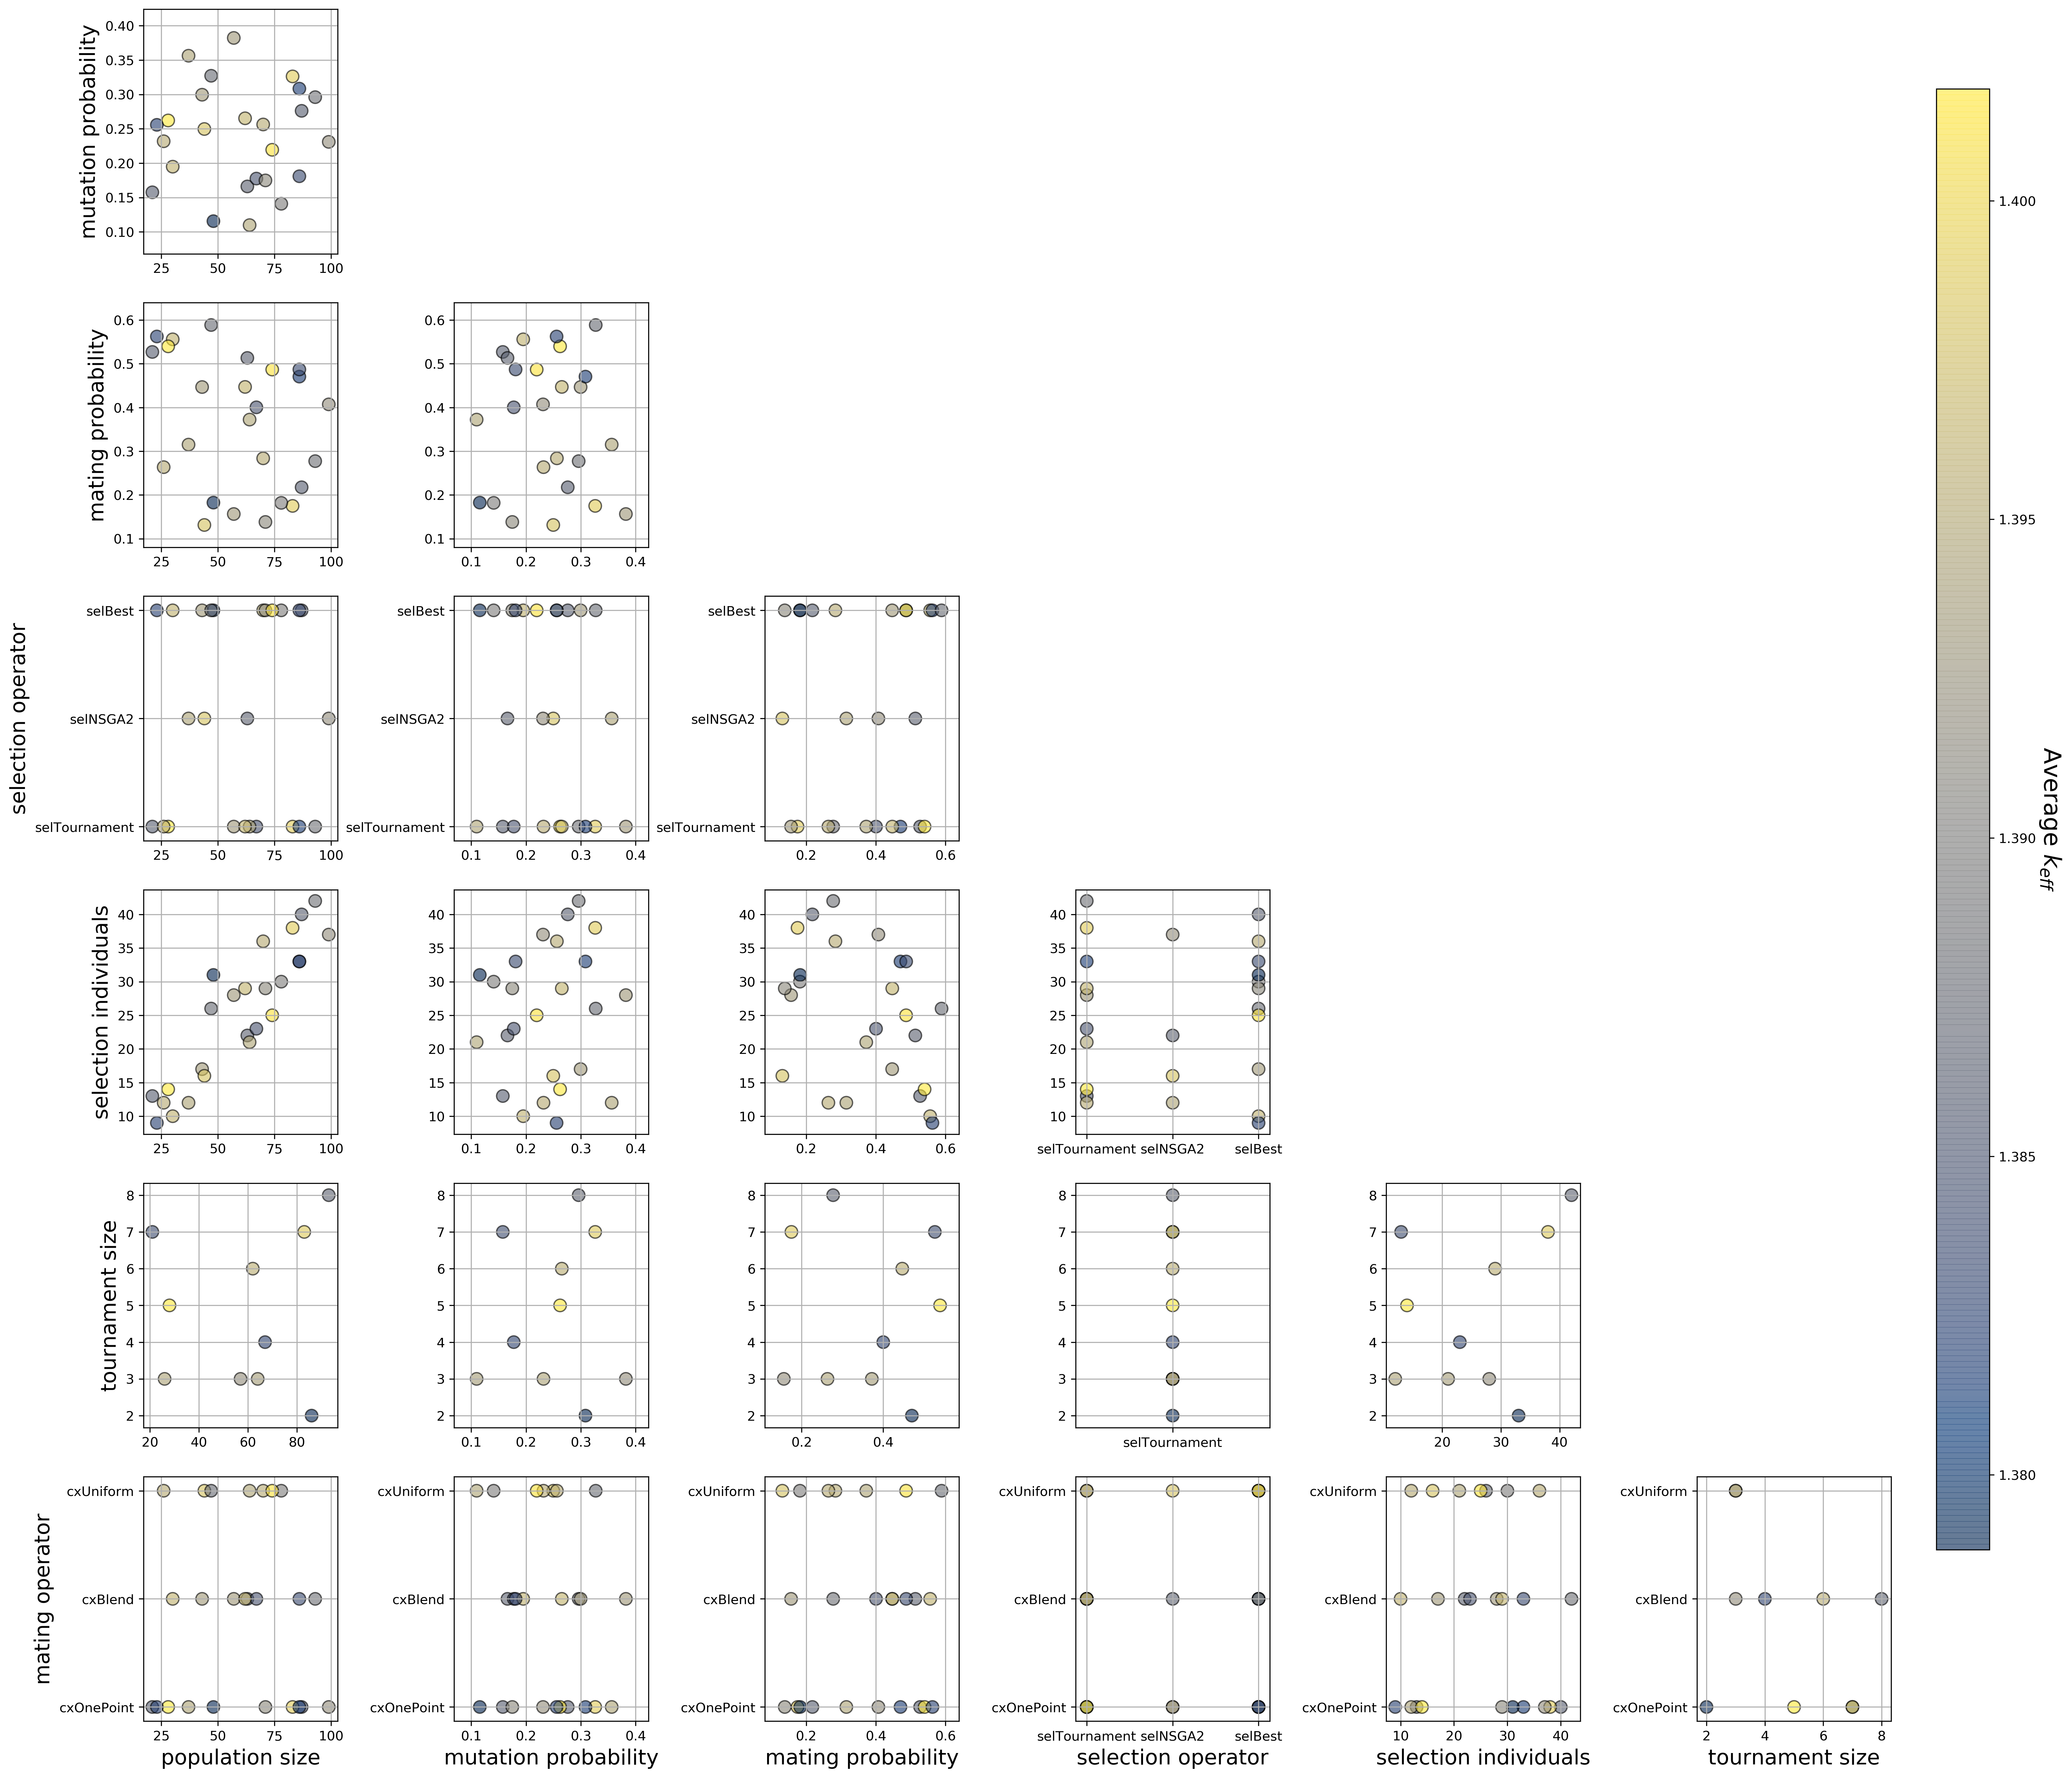
\includegraphics[width=1.3\linewidth]{hyperparameter_sens.png}} 
    \caption{Coarse hyperparameters search's results. Hyperparameter values are plotted 
    against each other with a third dimension of each experiment's final population's 
    average $k_{eff}$ indicated by each scatter point's color.}
    \label{fig:hyperparameter_sens}
\end{figure}
The hyperparameters are plotted against each other to visualize the interdependence 
between hyperparameters. 
From the coarse hyperparameter search, the trends that stood out were: 
\begin{itemize}
    \item Mutation probability has a larger $k_{eff ave}$ between 0.2 and 0.4. 
    \item Mating probability has a larger $k_{eff ave}$ when between 0.1 and 0.3. 
    \item Population size has a larger $k_{eff ave}$ when between 20 and 60. 
\end{itemize}
There is also not much interdependence between hyperparameters. 

Next, I proceeded to the fine search. 
From Figure \ref{fig:hyperparameter_sens}, I narrowed down population size, 
mutation probability, and mating probability bounds, as shown in Table 
\ref{tab:hyperparameter_search}'s \textit{Fine Search 1 Bounds} column. 
I did not see any significant trends in the other hyperparameters, so I chose 
to leave them as is. 
I ran ten more experiments (25 to 34) with sampling hyperparameters from 
the \textit{Fine Search 1 Bounds}. 
From these results, I conducted a second fine search with five experiments 
(35 to 39) with further tuned hyperparameter bounds as shown in Table 
\ref{tab:hyperparameter_search}'s \textit{Fine Search 2 Bounds} column. 
These new hyperparameter bounds were determined based on these reasons: 
\begin{itemize}
    \item Mutation probability has a larger $k_{eff ave}$ between 0.2 and 0.3.
    \item I overlooked a peaking of $k_{eff ave}$ at mating probability between 
    0.45 and 0.6 in the previous \textit{Fine Search 1}, thus shifted the bounds. 
    \item The highest $k_{eff ave}$ occurred for \texttt{selTournament}. 
    \item I narrowed down mating operator options to \texttt{cxBlend} and 
    \texttt{cxOnePoint} since they had higher $k_{eff ave}$. 
    \item I decided to select an arbitrary number for population size, 
    selection individuals, and tournament size since they did not appear to 
    correlate with $k_{eff ave}$ values. 
\end{itemize}
Figure \ref{fig:input_hyperparameters_sens} shows the relationship between 
hyperparameter values and $a$,$b$,$c$ input parameters, final generation 
$k_{eff max}$, and final generation $k_{eff ave}$. 
The coarse experiments' scatter points are $50\%$ transparent, while the fine 
experiments' scatter points are opaque. 
\begin{figure}[]
    \centering
    \makebox[\textwidth][c]{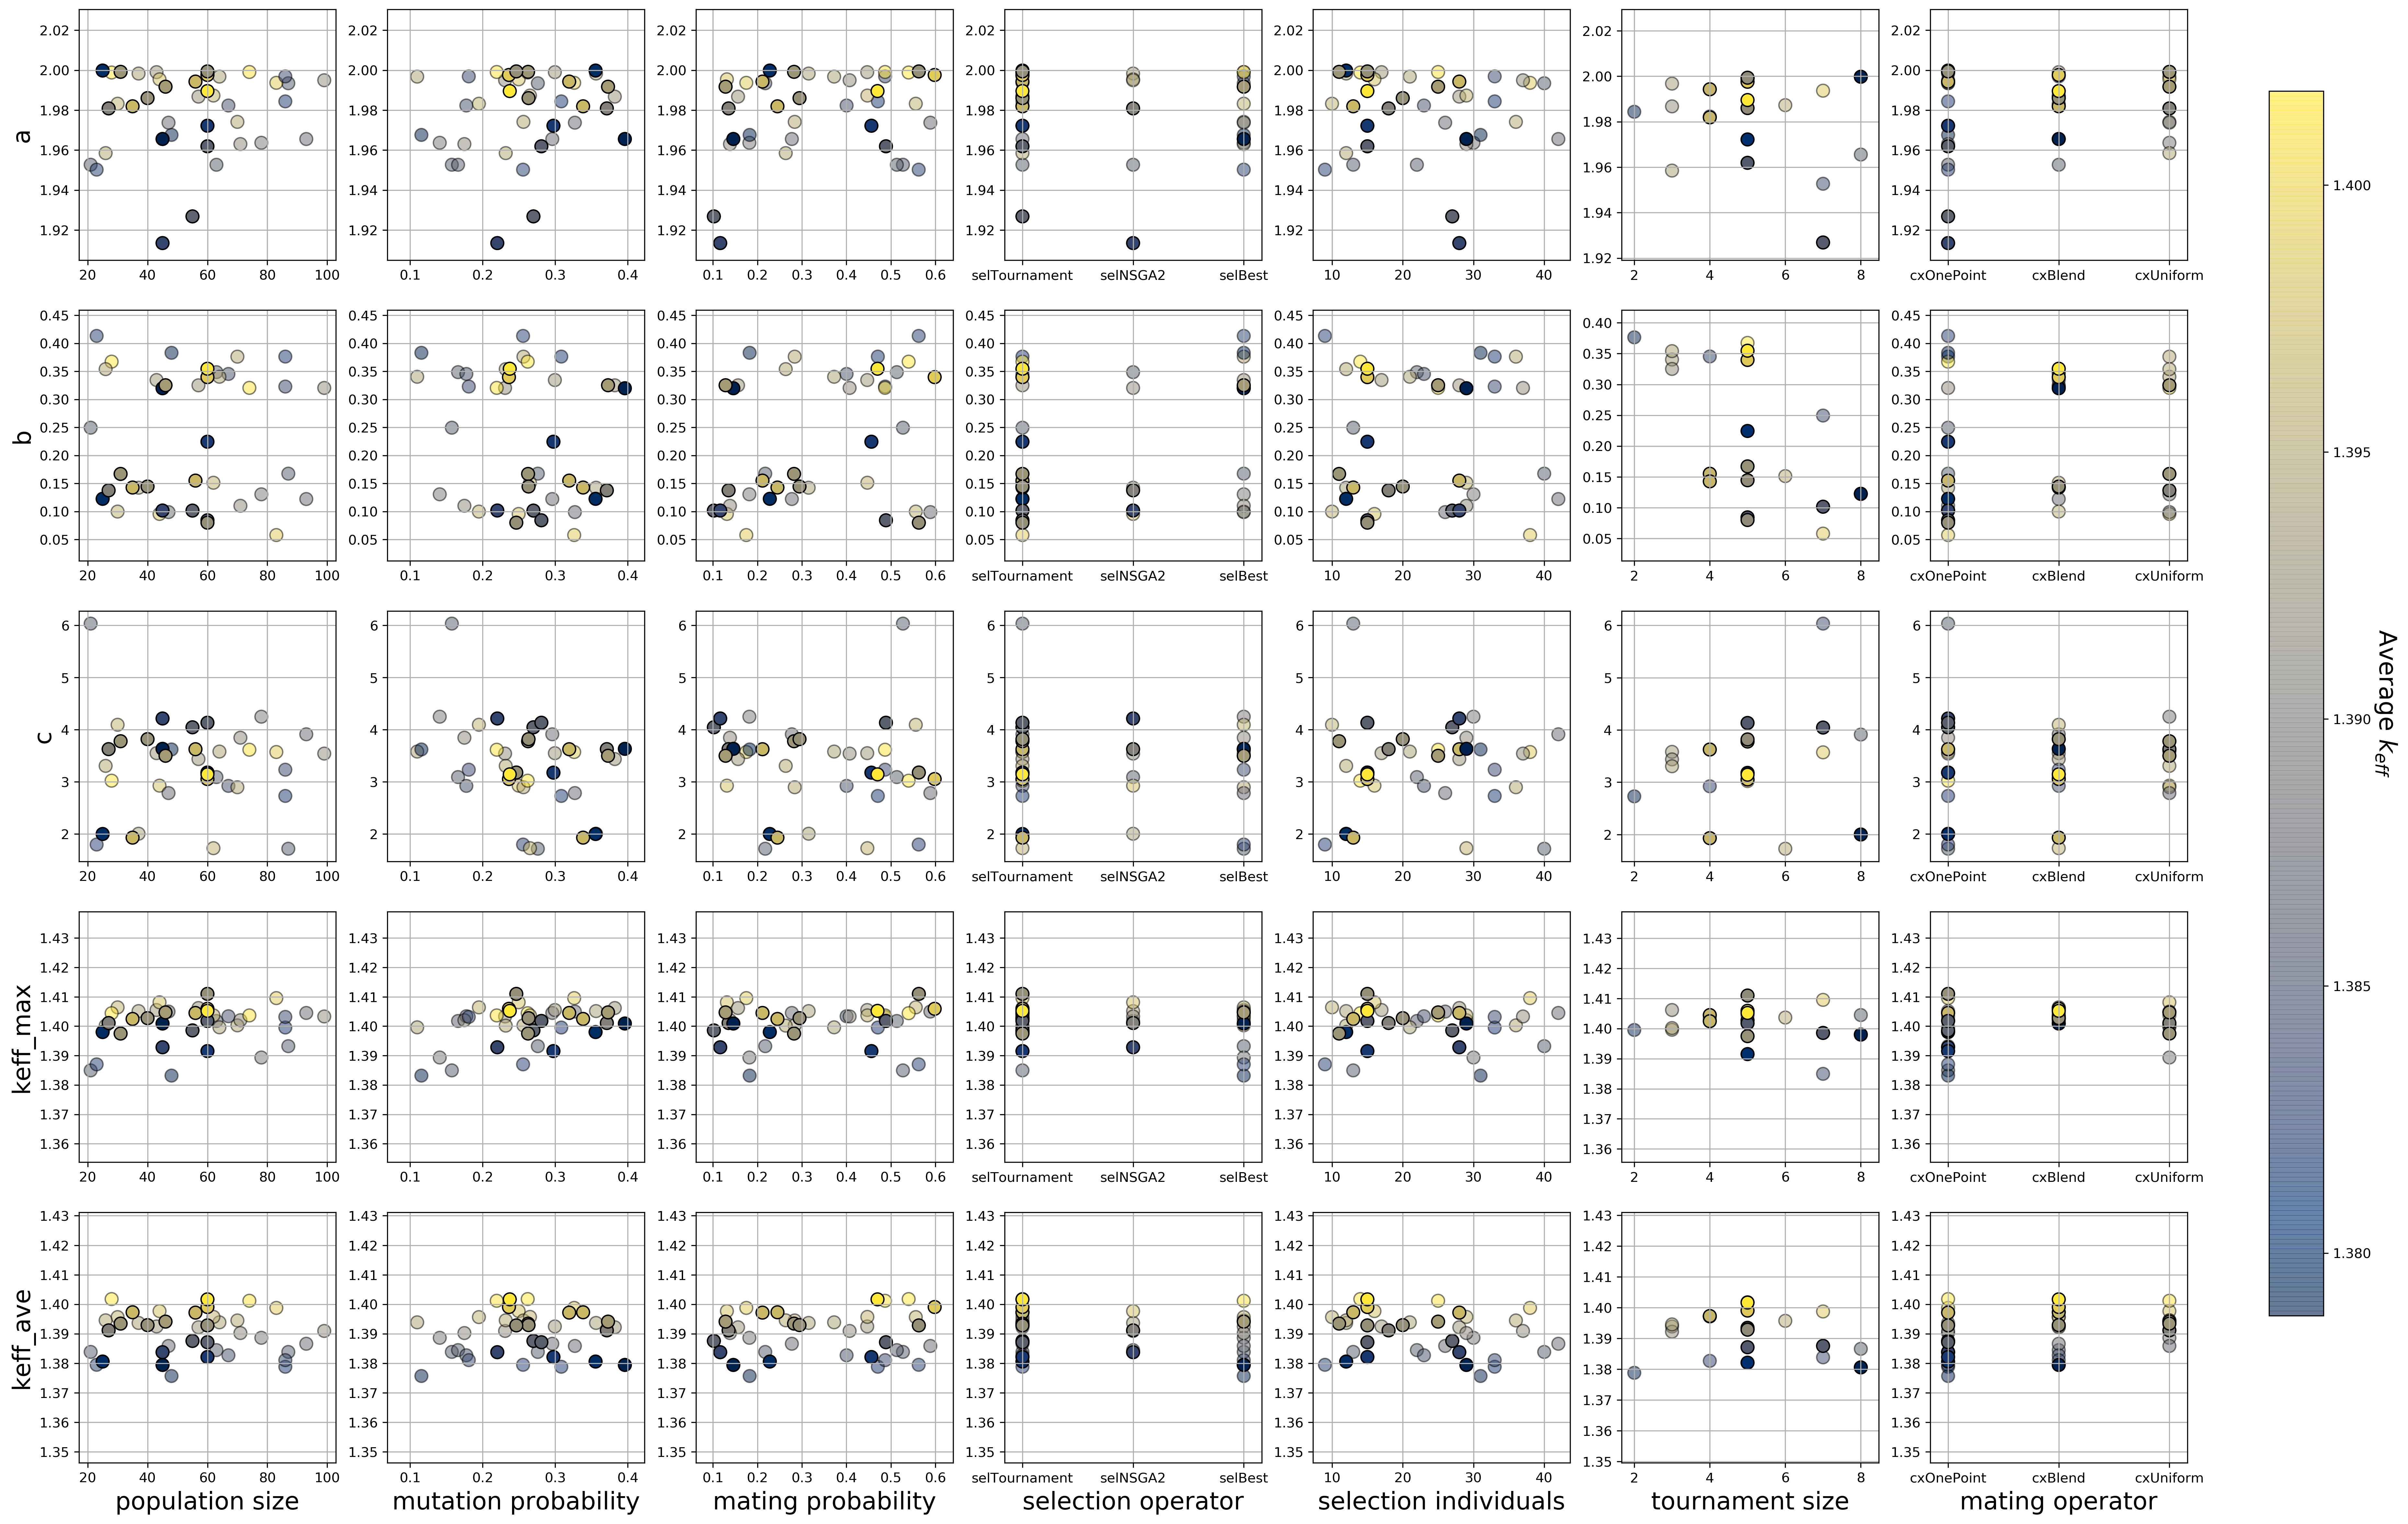
\includegraphics[width=1.3\linewidth]{input_hyperparameters_sens.png}} 
    \caption{Hyperparameters search's results. Hyperparameters are plotted 
    against a,b,c input parameters, each experiment's final generation
    $k_{eff max}$, and final generation $k_{eff ave}$ with a third dimension of 
    each experiment's final population's average $k_{eff}$ indicated by each 
    scatter point's color.}
    \label{fig:input_hyperparameters_sens}
\end{figure}
In Figure \ref{fig:input_hyperparameters_sens}, on average, the fine experiments 
(opaque scatter points) have higher $k_{eff ave}$, which indicates that the
hyperparameter search process met its objective of finding hyperparameter 
bounds that enable quicker and more accurate optimization. 

Table \ref{tab:topfive} shows the hyperparameters for the five experiments 
with the highest final generation $k_{eff ave}$.
\begin{table}[]
    \centering
    \onehalfspacing
    \caption{Input Parameters, $k_{eff}$ results, and hyperparameter values for 
    the five hyperparameter search experiments with the highest final generation 
    $k_{eff ave}$.}
	\label{tab:topfive}
    \footnotesize
    \makebox[\textwidth][c]{\begin{tabular}{p{3cm}p{3cm}p{3cm}p{3cm}p{3cm}p{3cm}}
    \hline 
    \textbf{Input/Output Parameters}& \textbf{Experiment 6} & \textbf{Experiment 15} & \textbf{Experiment 24} & \textbf{Experiment 36} & \textbf{Experiment 39}\\
    \hline 
    $k_{eff ave}$ & 1.39876 &1.40175&1.40118&1.39906&1.40165\\ 
    $k_{eff max}$ & 1.40954 &1.40440&1.40365&1.40590&1.40519\\ 
    a & 1.993&1.998&1.999&1.997&1.989\\
    b & 0.057&0.367&0.320&0.339&0.354\\ 
    c & 3.571&3.022&3.615&3.053&3.143\\
    \hline
    \textbf{Hyperparameter}& &&&&\\
    Population size & 83 & 28&74&60&60\\ 
    Generations &8&22&9&10&10 \\
    Mutation probability & 0.32 &0.26&0.21&0.23&0.23\\
    Mating probability & 0.17 &0.53&0.48&0.59&0.46\\
    Selection operator & \texttt{selTournament} &\texttt{selTournament}&\texttt{selBest}&\texttt{selTournament}&\texttt{selTournament}\\
    Selection individuals & 38 &14&25&15&15\\
    Selection tournament size & 7 &5&-&5&5\\
    Mutation Operator & \texttt{mutPolynomial} \texttt{Bounded}&\texttt{mutPolynomial} \texttt{Bounded}&\texttt{mutPolynomial} \texttt{Bounded}&\texttt{mutPolynomial} \texttt{Bounded}&\texttt{mutPolynomial} \texttt{Bounded}\\
    Mating Operator & \texttt{cxOnePoint} &\texttt{cxOnePoint}&\texttt{cxUniform}&\texttt{cxBlend}&\texttt{cxBlend}\\ 
    \hline
    \end{tabular}}
\end{table}
Figure \ref{fig:topfiveplot} shows the packing fraction distributions that 
produced the $k_{eff max}$ from each of the top five experiments. 
\begin{figure}[]
    \centering
    \makebox[\textwidth][c]{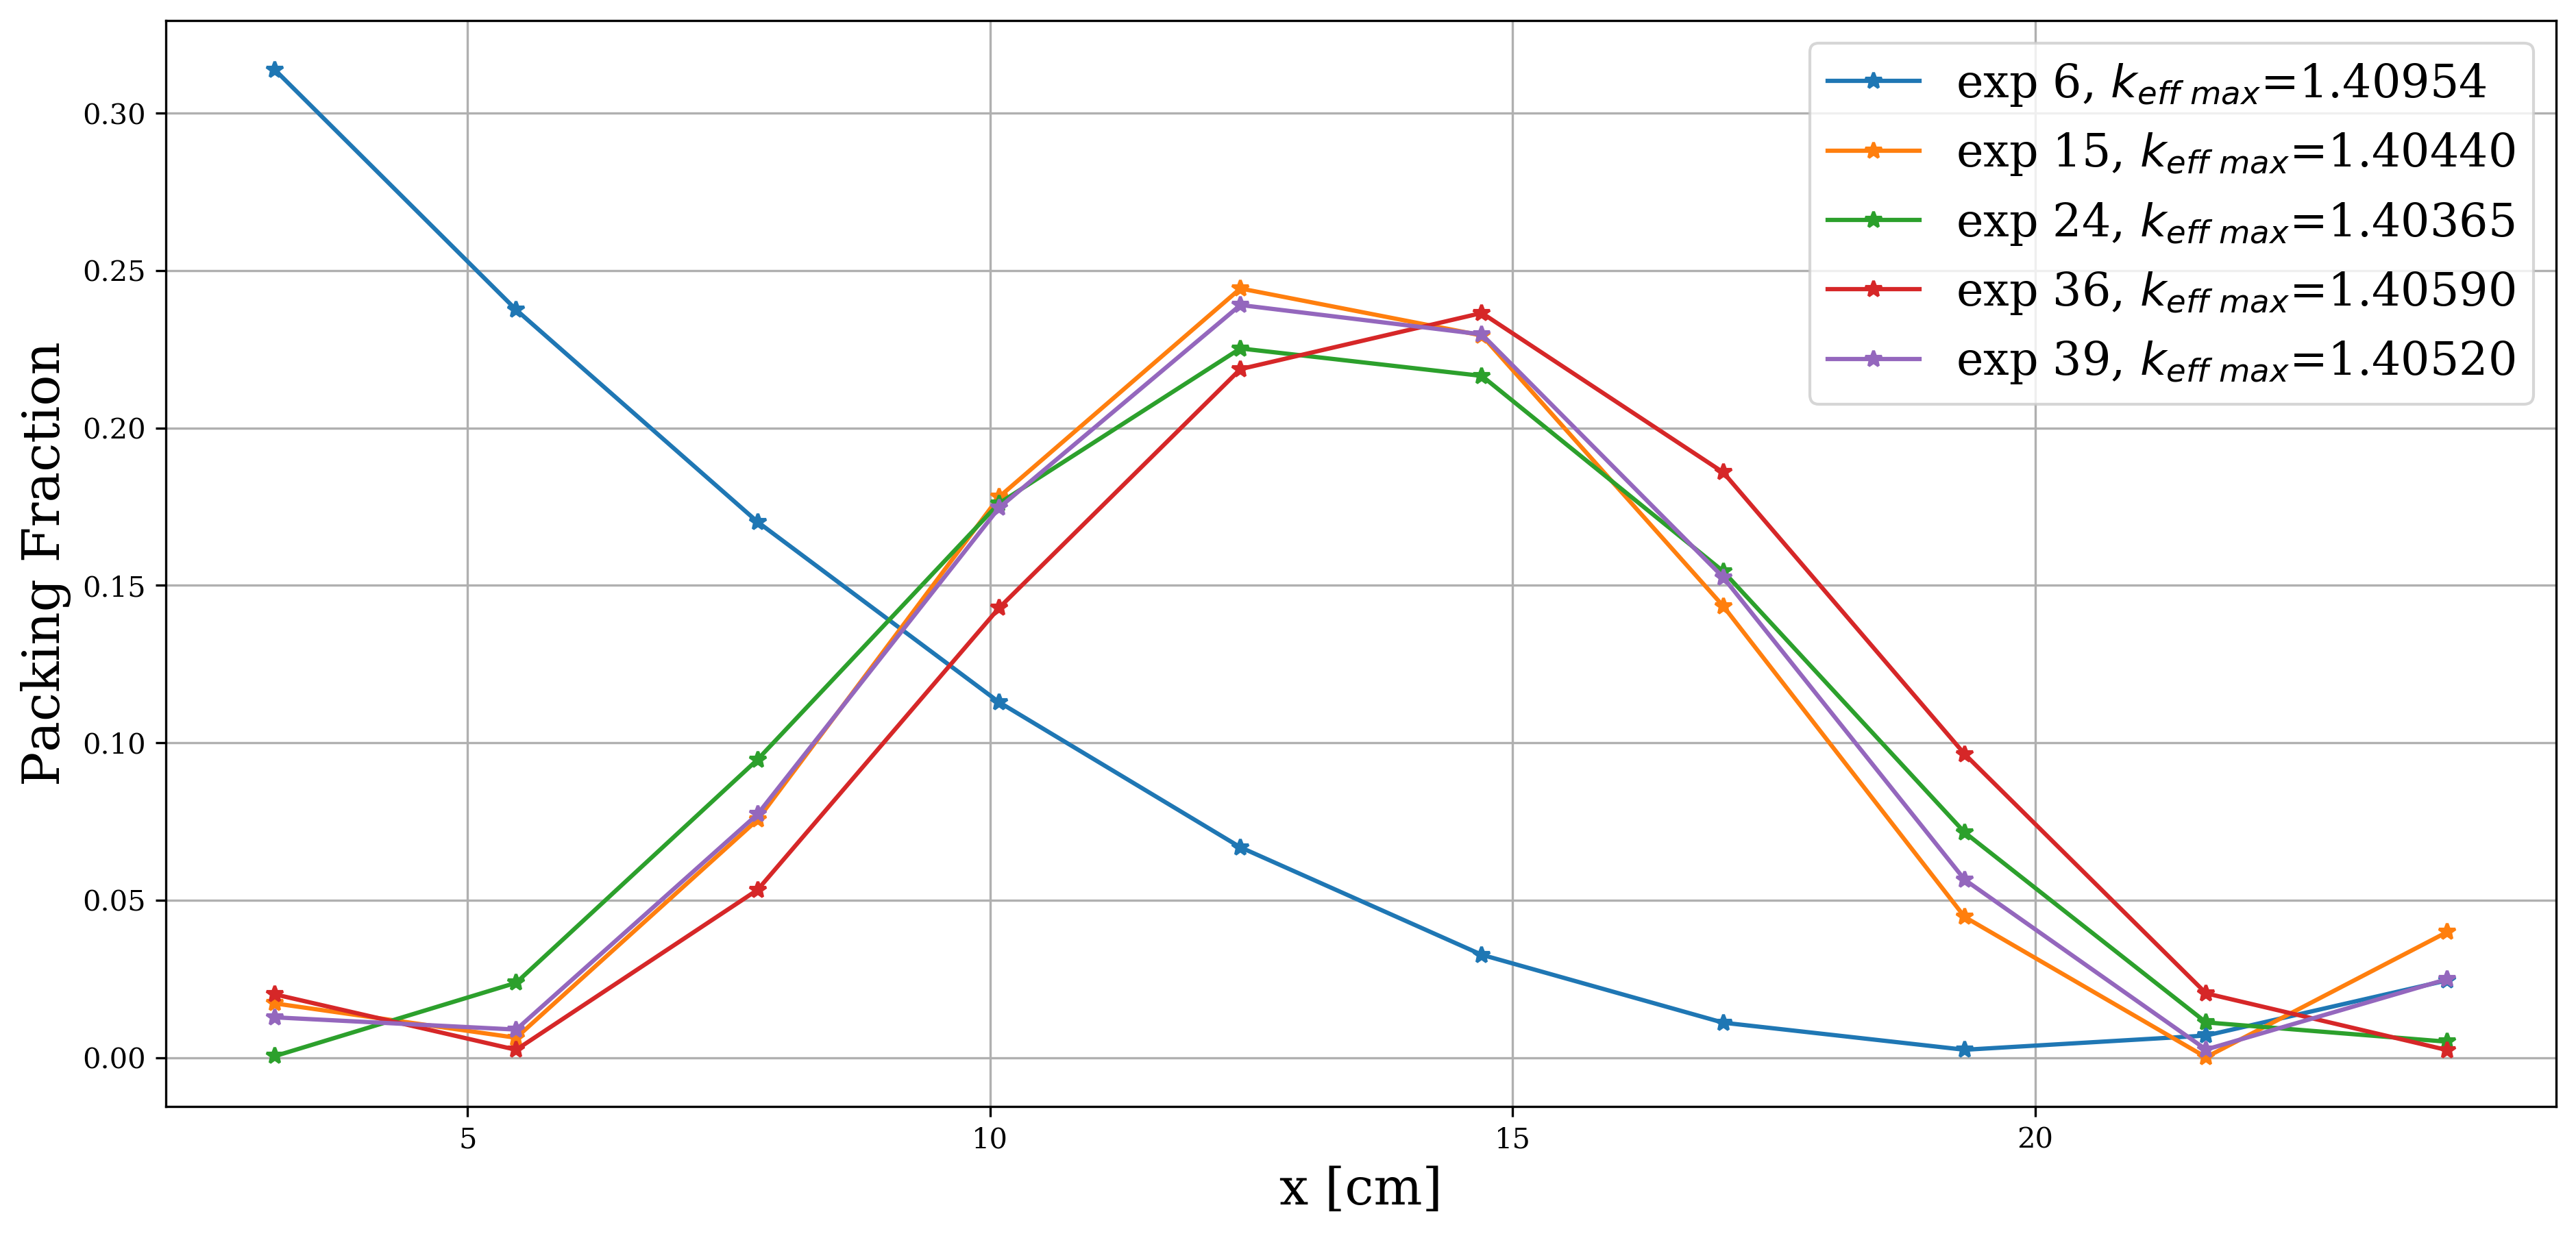
\includegraphics[width=1\linewidth]{topfive_plot.png}} 
    \caption{}
    \label{fig:topfiveplot}
\end{figure}
Four experiments had similar distributions of packing fraction peaking at approximately 
0.23 in the center of the slab, while one experiment had an exponential-looking 
distribution with peak packing fraction of 0.31 at the side of the slab.
The similar final packing fraction distributions demonstrate the robustness of 
genetic algorithms to find the optimal global solutions with different 
hyperparameters. 

These simulations are run on the BlueWaters supercomputer \cite{ncsa_about_2017}. 
In each \gls{REALM} simulation, a population size number of individual OpenMC 
simulations are run at each generation. 
Each OpenMC simulation takes approximately 13 minutes to run on a single BlueWaters 
XE node. 
With approximately 600 OpenMC evaluations per \gls{REALM} simulation, the total 
\gls{REALM} simulation time is about 130 BlueWaters node-hours. 
The hyperparameter search ran 40 REALM simulations, thus using approximately
5200 node-hours.

\subsection{Results for best hyperparameter set}
I define the best-performing hyperparameter set as the experiment that produces 
the highest $k_{eff ave}$ in its final generation. 
The best performing set of hyperparameters is from the final 
\textit{Fine Search 2}. 
It is experiment 39 in Table \ref{tab:topfive} with center-peaking packing 
fraction distribution with $k_{eff max} = 1.40519$. 
Experiment 39's $k_{eff max}$ is $\sim2000$pcm larger than the original 
straightened \gls{AHTR} configuration's $k_{eff}$. 
Figures \ref{fig:triso_distribution_sine_39} show the packing fraction distribution 
that produced $k_{eff max} = 1.40519$. 
\begin{figure}[]
    \centering
    \makebox[\textwidth][c]{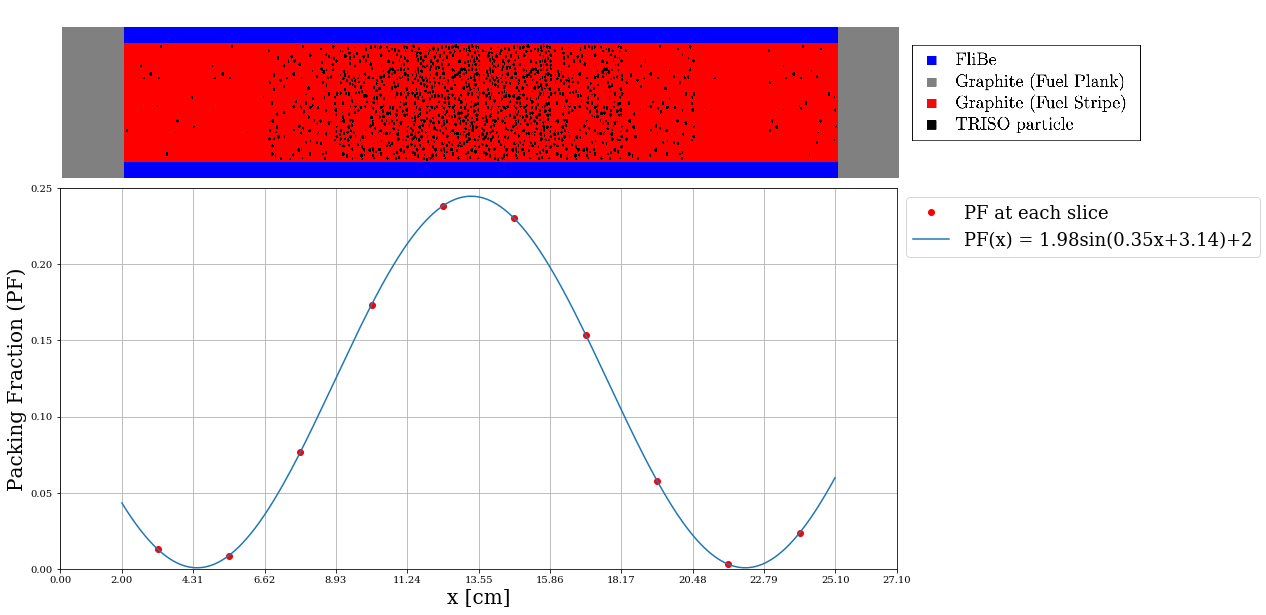
\includegraphics[width=1.1\linewidth]{triso_distribution_sine_39.png}} 
    \caption{Experiment 39 packing distribution that produced $k_{eff max} = 1.40519$. 
    Below: $PF(x) = (1.98\ sin(0.35x+3.14)+2)  \times NF$ sine distribution with 
    red points indicating the packing fraction at each slice. 
    Above: Straightened \acrlong{AHTR} fuel slab with varying \gls{TRISO} particle 
    distribution across ten slices based on the sine distribution. }
    \label{fig:triso_distribution_sine_39}
\end{figure}

Figure \ref{fig:keff_conv_39} and \ref{fig:pf_39} show the evolution of $k_{eff}$ 
and packing fraction distribution through each generation of the best performing 
39$^{th}$ experiment.
\begin{figure}[]
    \centering
    \begin{subfigure}{\textwidth}
    \makebox[\textwidth][c]{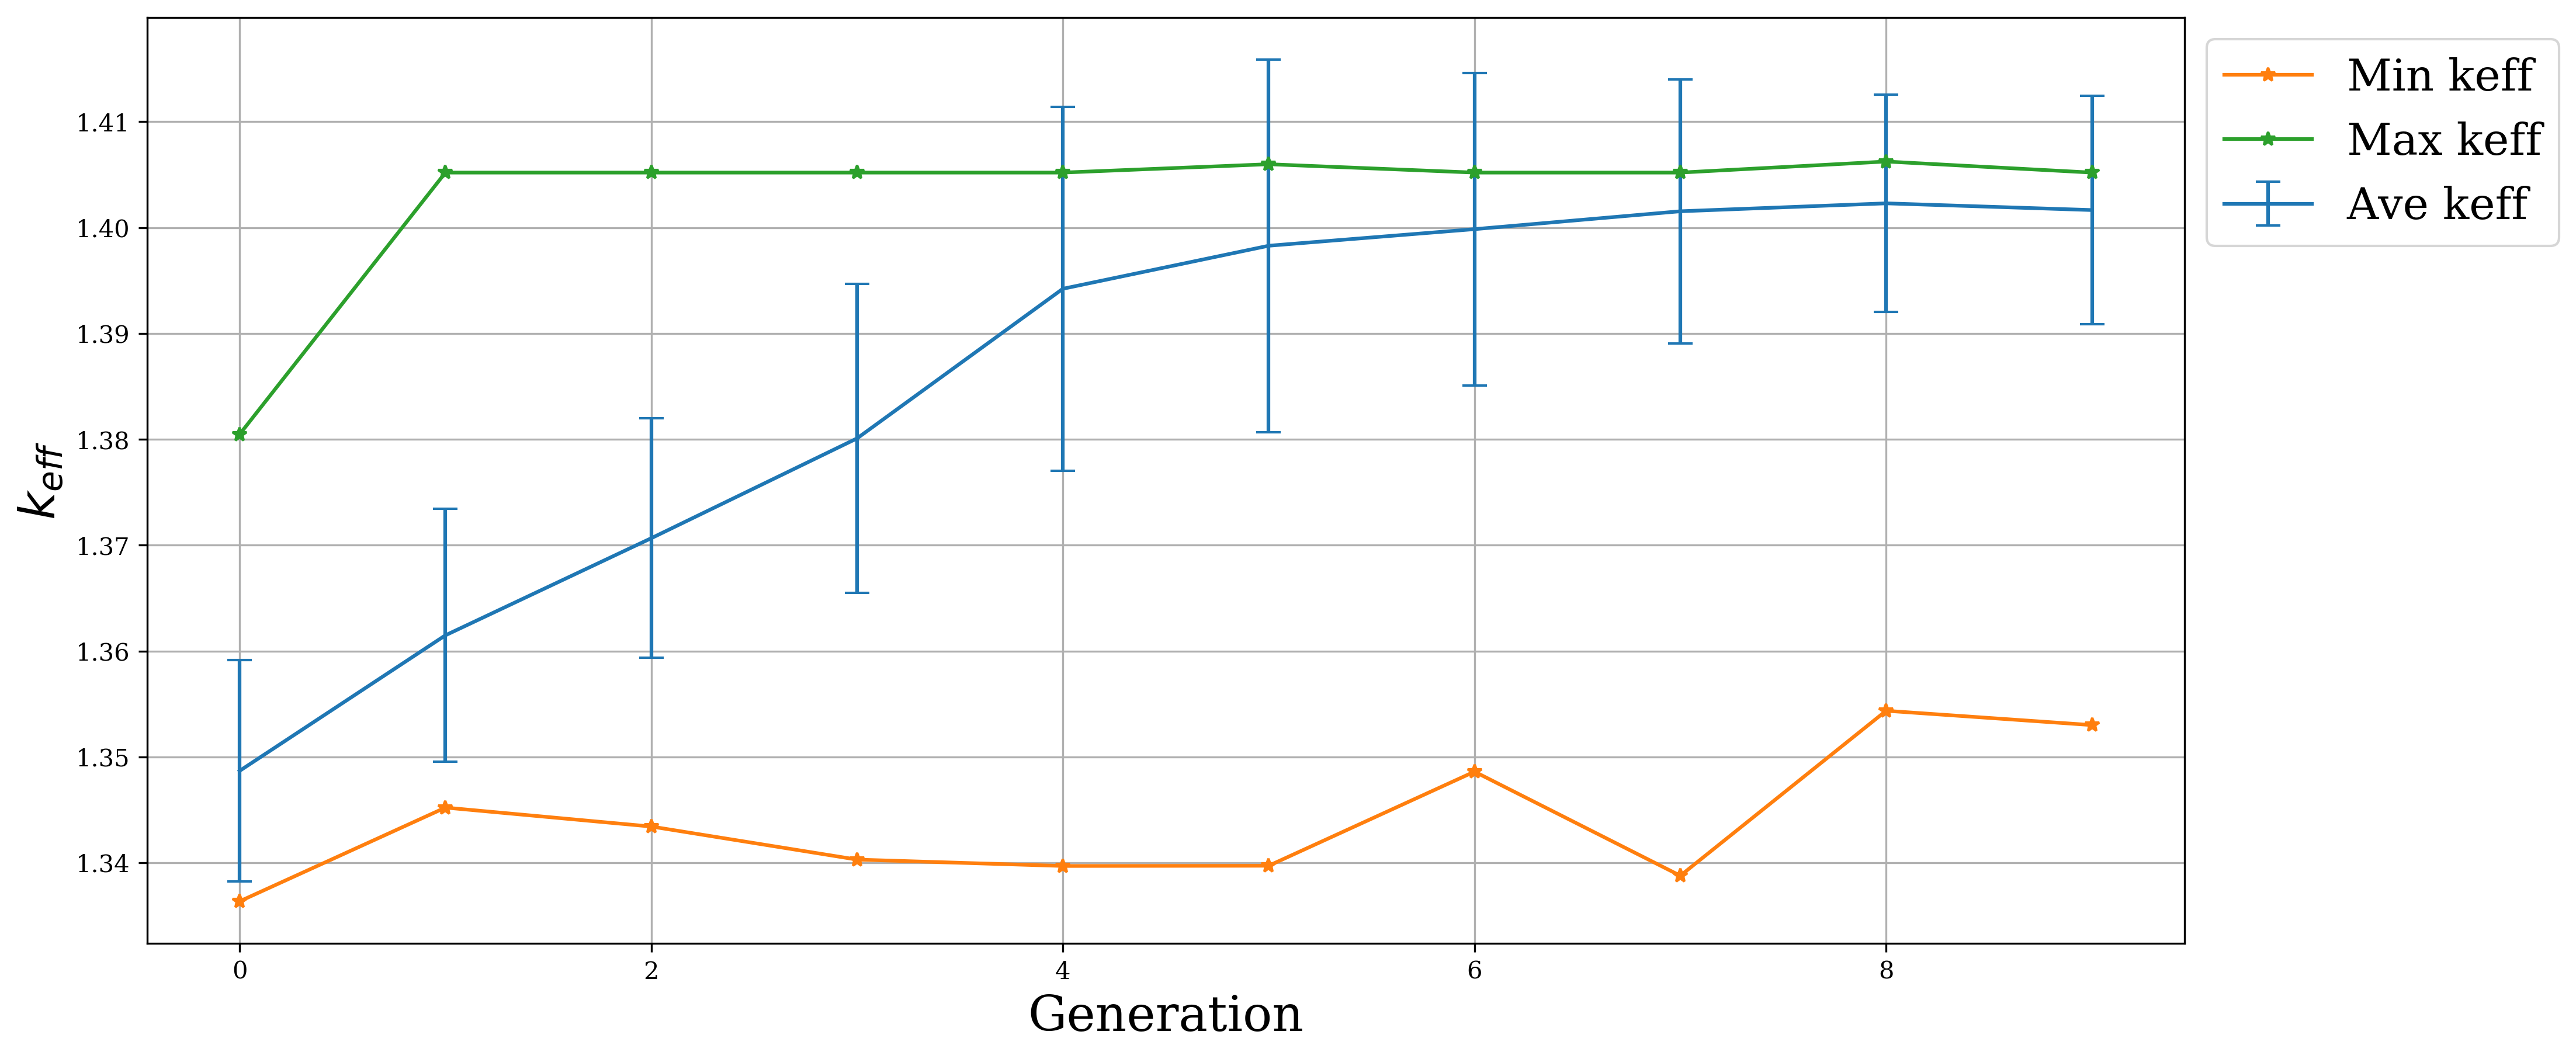
\includegraphics[width=1.1\linewidth]{keff_conv_39.png}} 
    \caption{Minimum, average, and maximum $k_{eff}$ values evolution.}
    \label{fig:keff_conv_39}
    \end{subfigure}
    \begin{subfigure}{\textwidth}
        \makebox[\textwidth][c]{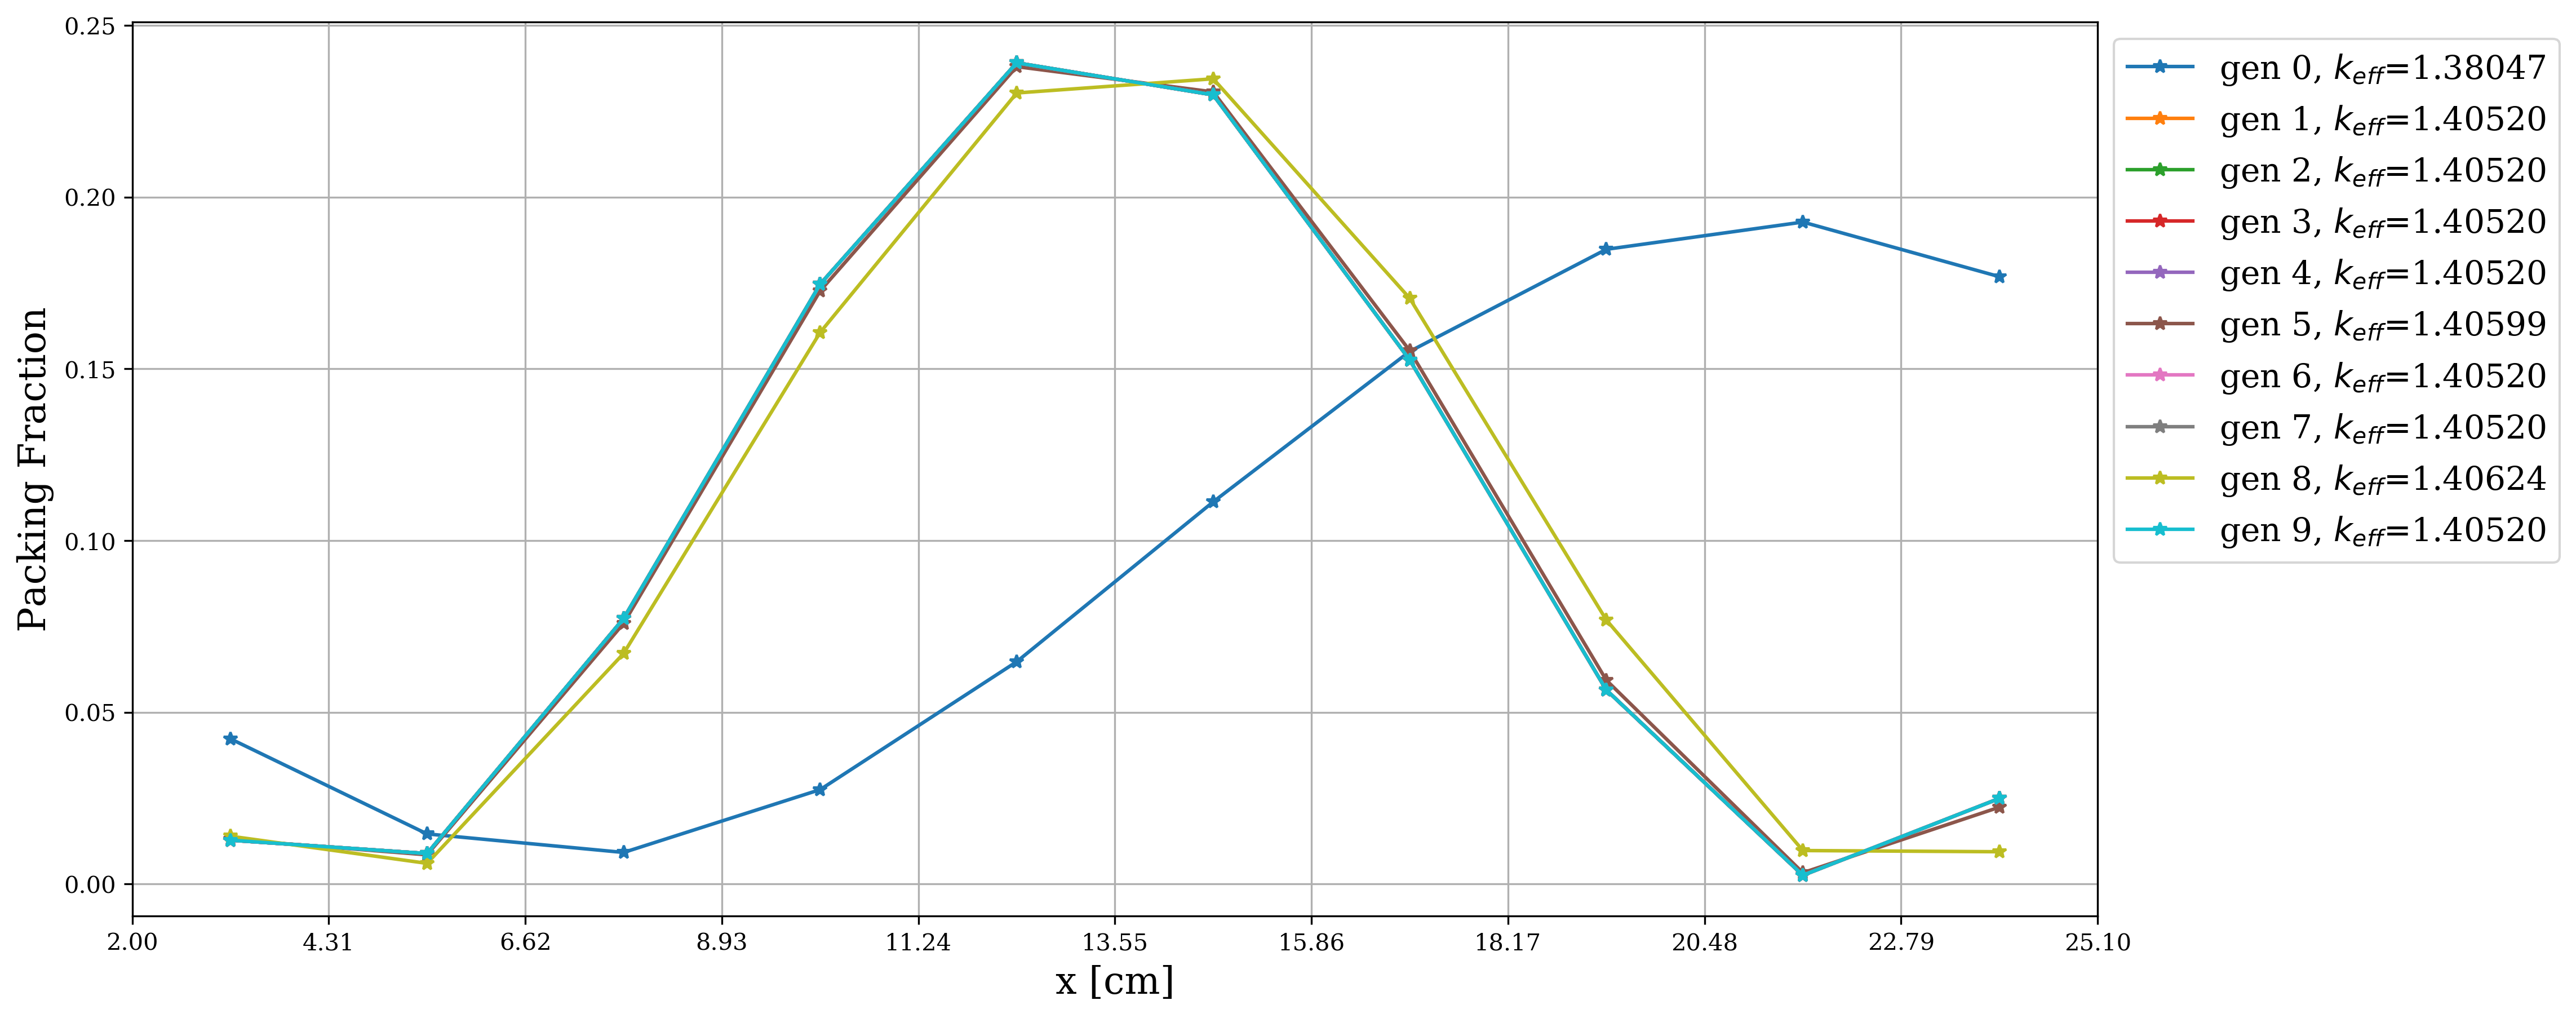
\includegraphics[width=1.1\linewidth]{pf_39.png}} 
        \caption{Maximum $k_{eff}$'s packing fraction distribution evolution.}
        \label{fig:pf_39}
    \end{subfigure}
    \caption{ Results for each generation for \gls{REALM}'s genetic algorithm optimization 
    of the Straightened \acrfull{AHTR} Fuel Slab. The \gls{REALM} simulation used 
    the 39$^{th}$ experiment's hyperparameter set.}
    \label{fig:39}
\end{figure}
The $k_{eff max}$ converged quickly by generation 1; however, this is not 
usually the case. 
The genetic algorithm optimization process is stochastic, and so there is always 
the possibility that the algorithm randomly samples a set of input parameters
that maximizes the objective function early on in the genetic algorithm 
optimization process. 
The $k_{eff ave}$ demonstrates how each generation's average $k_{eff}$
converges towards a higher value with each generation's improvements
To demonstrate how the genetic algorithm optimization process usually goes, 
Figures \ref{fig:keff_conv_15} and \ref{fig:pf_15} show the evolution of $k_{eff}$ 
and packing fraction distribution through each generation of the second-best 
performing 15$^{th}$ experiment, respectively. 
Experiment 15 demonstrates how both maximum and average $k_{eff}$ converges 
towards a higher $k_{eff}$ with improvements from each generation.
\begin{figure}[]
    \centering
    \begin{subfigure}{\textwidth}
    \makebox[\textwidth][c]{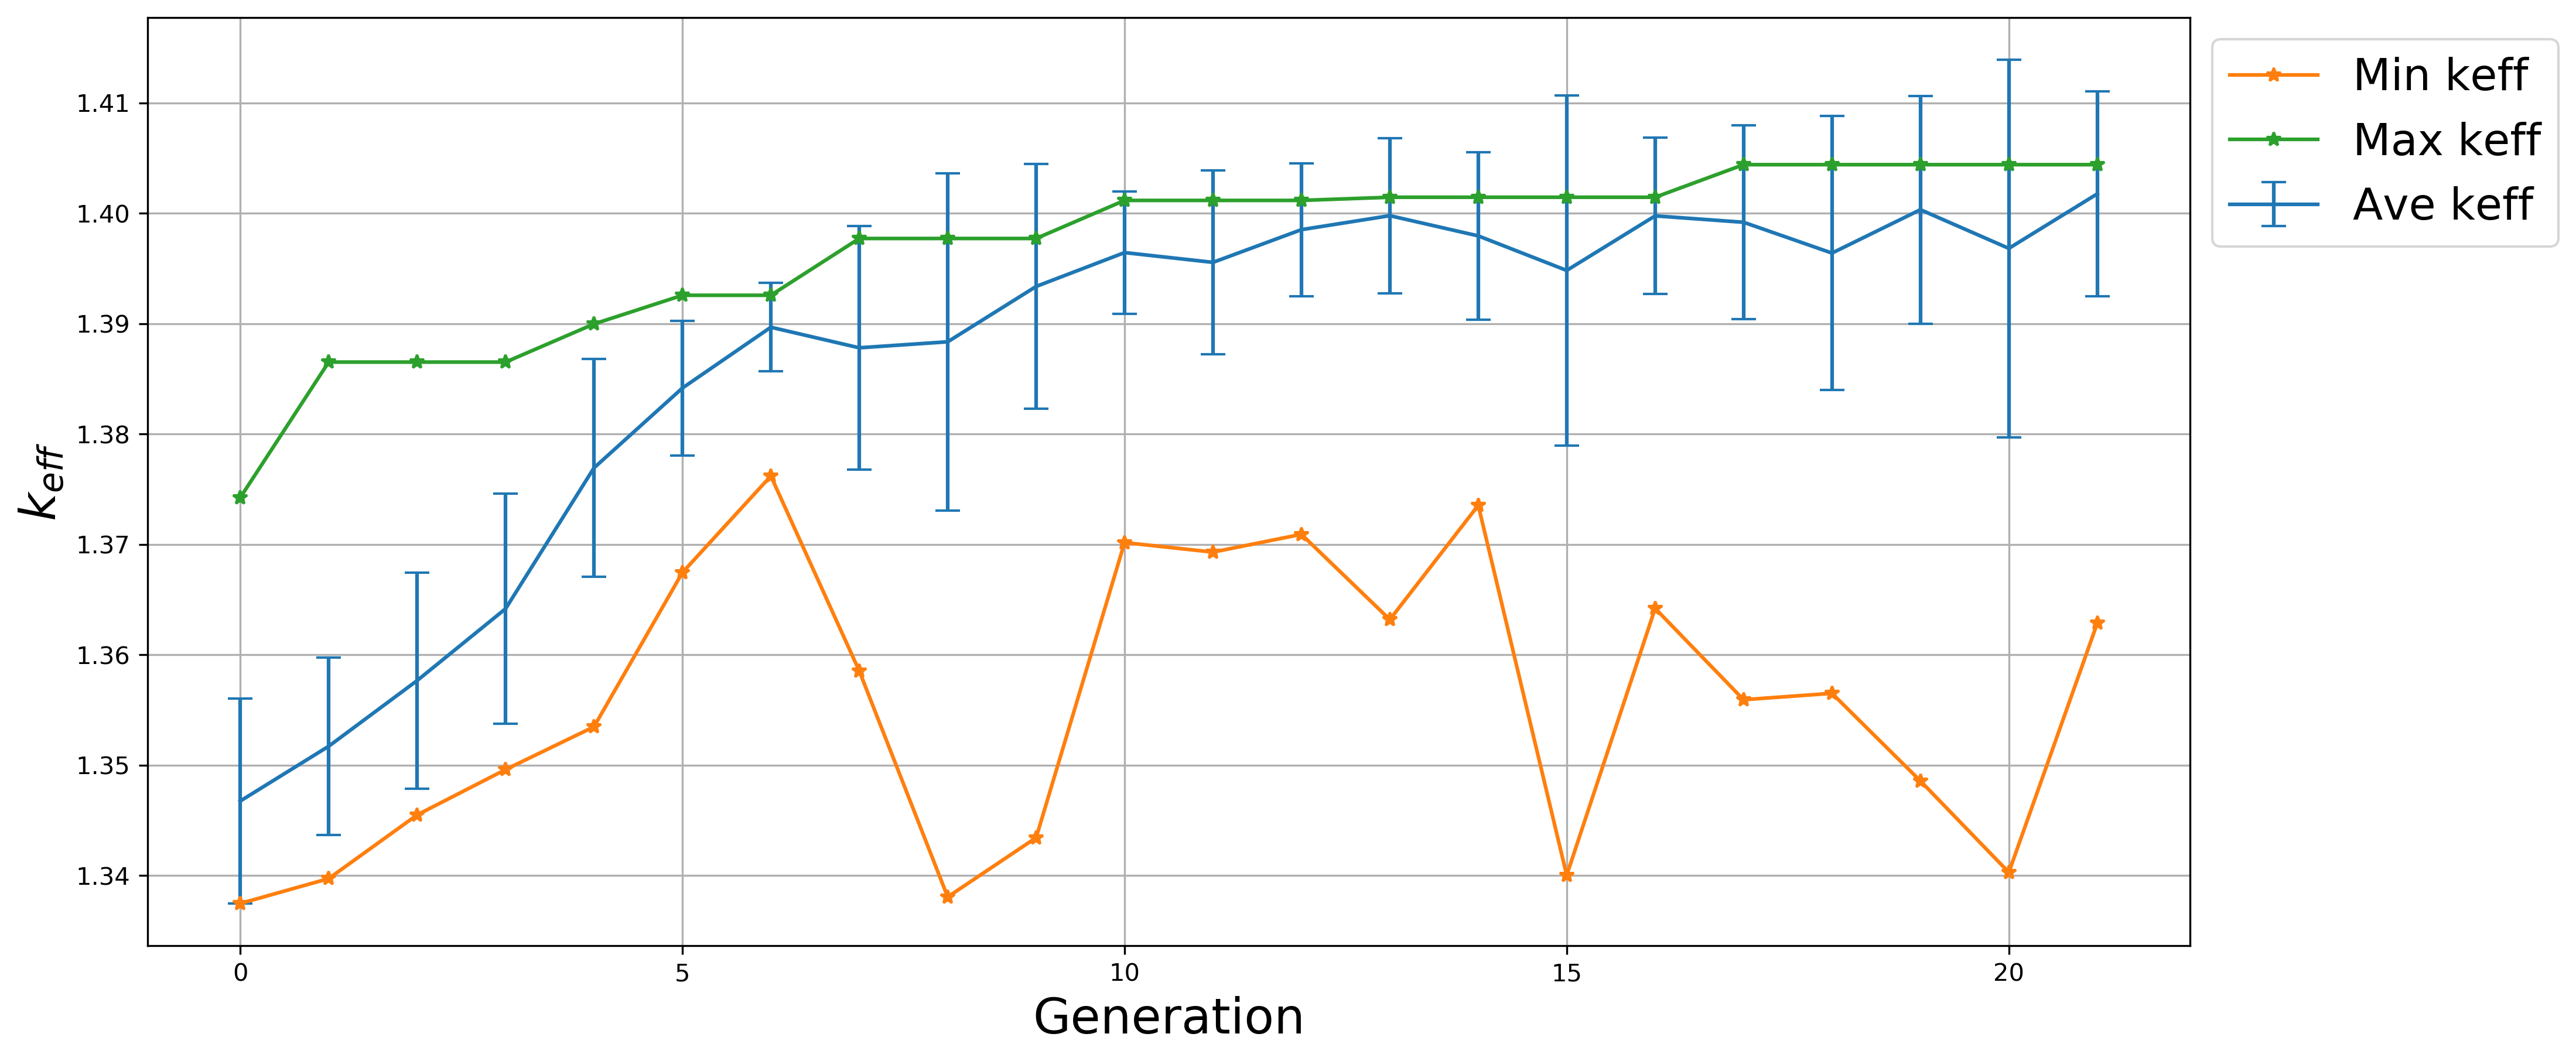
\includegraphics[width=1.1\linewidth]{keff_conv_15.png}} 
    \caption{Minimum, average, and maximum $k_{eff}$ values evolution.}
    \label{fig:keff_conv_15}
    \end{subfigure}
    \begin{subfigure}{\textwidth}
        \makebox[\textwidth][c]{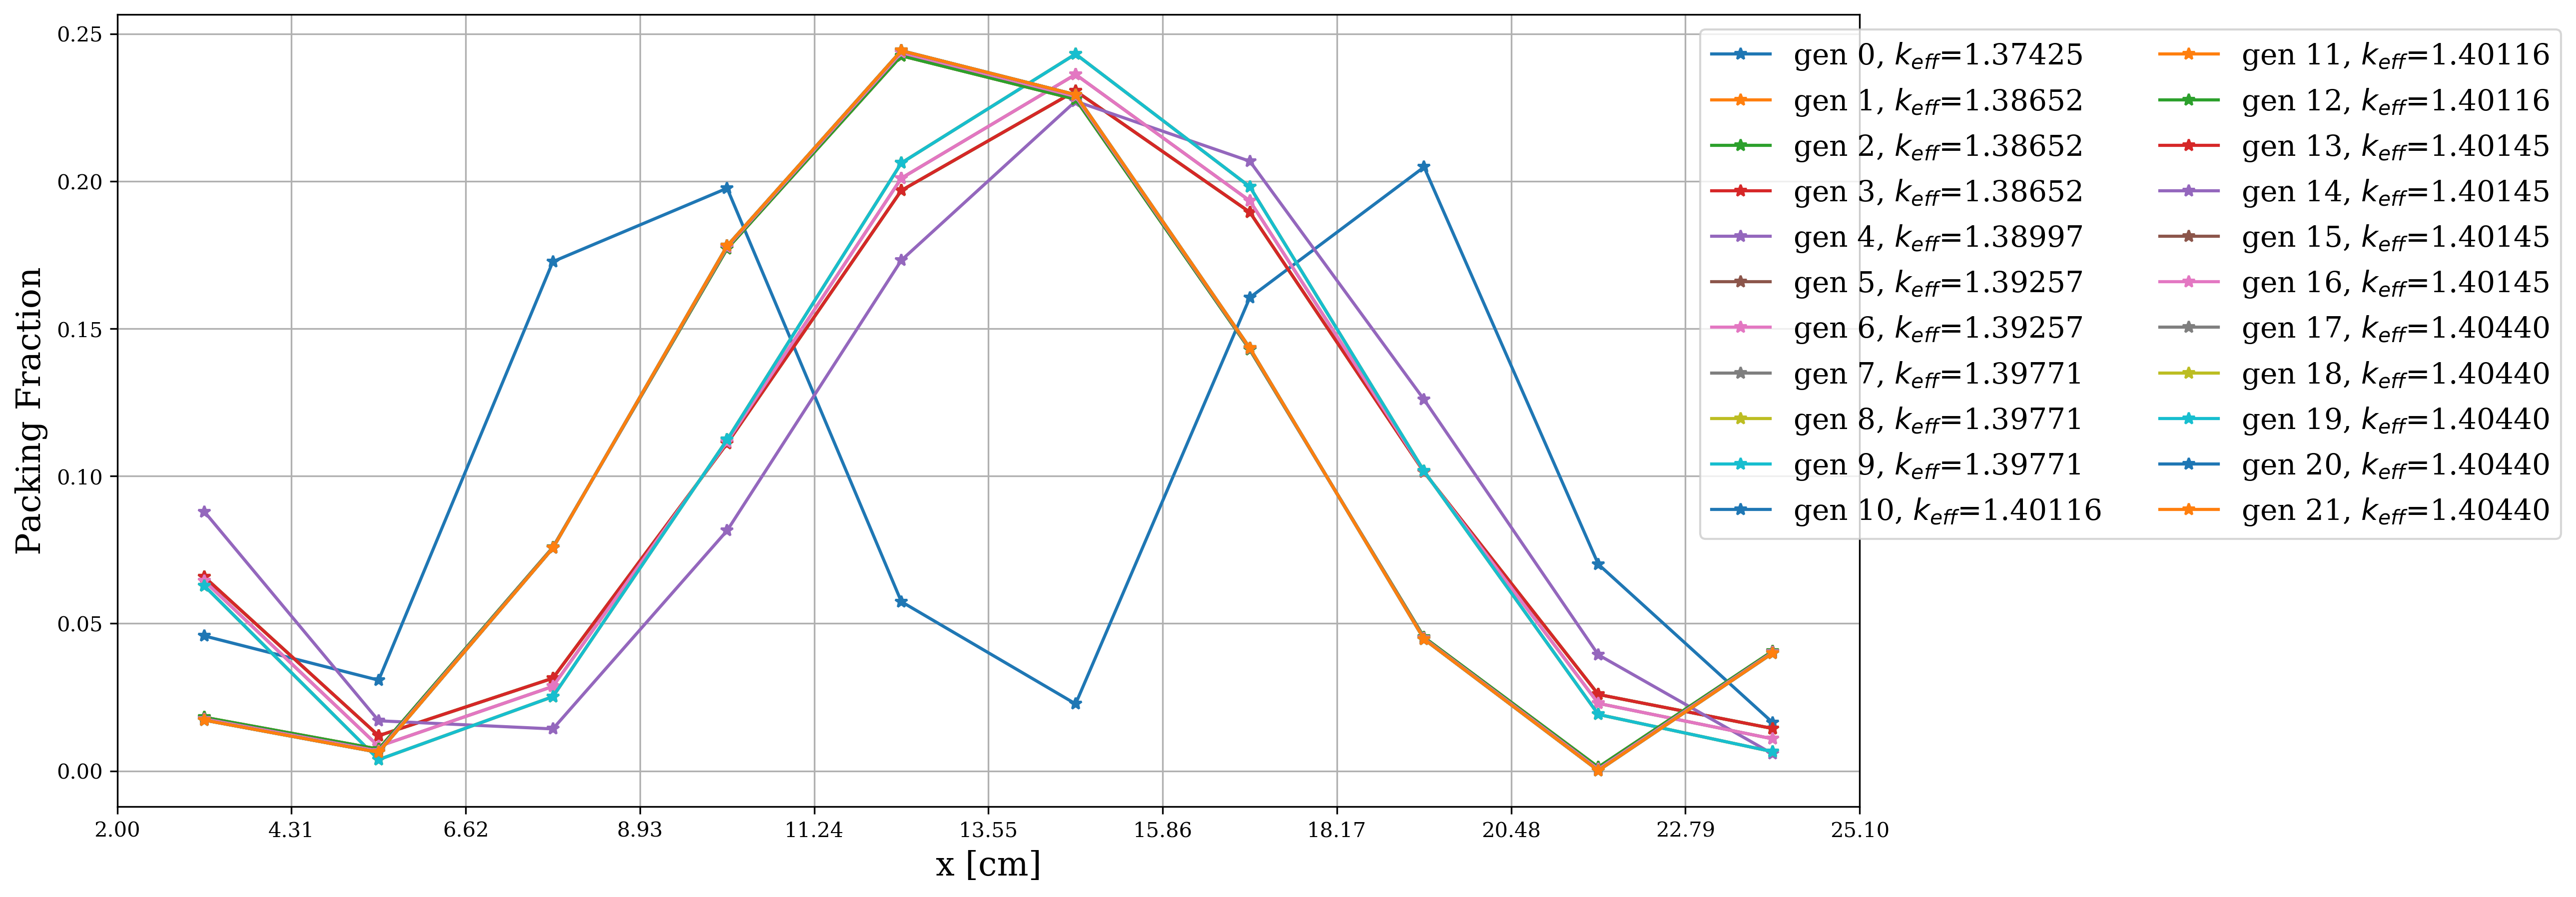
\includegraphics[width=1.1\linewidth]{pf_15.png}} 
        \caption{Maximum $k_{eff}$'s packing fraction distribution evolution.}
        \label{fig:pf_15}
    \end{subfigure}
    \caption{ Results for each generation for \gls{REALM}'s genetic algorithm optimization 
    of the Straightened \acrfull{AHTR} Fuel Slab. The \gls{REALM} simulation used 
    the 15$^{th}$ experiment's hyperparameter set.}
    \label{fig:15}
\end{figure}

Both experiments 39 and 15 have packing fractions peaking at approximately 
0.23 in the center of the slab and decreasing to zero at the slab's sides.  
The amplitude, $a$, for the packing fraction distribution that produced $k_{eff max}$ 
for experiment 39 and the other top-five experiments (Table \ref{tab:topfive}) 
have settled at the upper bound of approximately 2. 
A higher amplitude, $a$, shows that a slab geometry with larger variations of 
packing fraction results in a larger $k_{eff}$. 
These observations about packing fraction distribution for $k_{eff max}$ are 
consistent with what I understand from the original \gls{AHTR}: a high $k_{eff}$ 
occurs when there is a good balance between fuel loading and moderation space. 
Fission occurs at areas of high \gls{TRISO} particle concentration at thermal flux;
however, the neutrons are born at fast-flux and require moderation to slow down 
to thermal ranges.
Therefore, larger moderation areas ensure higher resonance escape probability for 
the fast neutrons resulting in higher thermal flux, leading to more 
fission occurring and a higher $k_{eff}$. 

Another observation is that TRISO particles peak in the center of the slab, 
proving that when the optimization problem focuses purely on the slab's neutronics 
by maximizing $k_{eff}$, the fuel tends to want to culminate in the middle. 
However, this is not ideal for other important reactor core qualities such as 
good heat transfer and ensuring flat power across the core. 
With these shortcomings in mind, I proceed to the future work chapter to discuss 
the types of simulations that will be run to optimize these other parameters. 

\section{Summary}
This chapter demonstrated successfully applying \gls{REALM} to maximize $k_{eff}$ 
in a straightened \acrfull{AHTR} fuel slab through varying the \gls{TRISO} 
particle packing fraction distribution. 
I began by conducting a coarse-to-fine random sampling hyperparameter search to 
find the genetic algorithm hyperparameters that worked best for this optimization 
problem.
Experiment 39 performed the best with a hyperparameter set that produced the 
highest final generation average $k_{eff}$ of 1.40165. 
The \gls{TRISO} particle packing fraction distribution that produced the final 
generation's maximum $k_{eff}$ of 1.40519 peaks at the center of the slab with 
a packing fraction distribution of $PF(x)=1.989\ sin(0.54x+3.143)$. 
This problem demonstrated how effective and robust genetic algorithms are for 
optimizing reactor parameters for an objective function. 
This demonstration problem had a single objective function which was to maximize 
$k_{eff}$. 
However, many other objectives should be considered, such as maximizing heat 
transfer and minimizing power peaking in the core.
Thus, in the next chapter, I propose future simulations for optimizing
these objective functions simultaneously.

%\chapter{Future Work and Proposed Simulations}
% Main Gist 
% - My planned work
% Structure 
% - Stage 1: Tune hyperparameters for moltres problem
% - Stage 2: Demonstration of realm with moltres with complicated problem 
% - Stage 3: Evaluate the moltres' heat transfer interface and improve on it


% multi objective -> maximize keff, minimize power peaking / maximize heat transfer 
% These ideas lead into the proposal section 

% IDEAS 
% vary in y direction 
% try the whole 1/3 diamond fuel elemt 

The need for this work is shown by a summary of how additive manufacturing 
of nuclear reactor core components frees complex reactor geometries from 
previous manufacturing constraints enabling reactor designers to reexamine 
reactor core design optimization.
The literature review (Chapter \ref{chap:lit-review}) concluded that stochastic 
evolutionary algorithm optimization methods can be leveraged to find global 
optimums for reactor design problems in the vast exploration design space 
enabled by additive manufacturing. 
Chapter \ref{chap:fhr-benchmark} introduced the \acrfull{AHTR} benchmark and 
highlighted the reactor's benefits such as passive safety behavior with negative 
temperature coefficients. 
In Chapter \ref{chap:realm}, I introduced the \acrfull{REALM} software package 
which applies evolutionary algorithm optimization techniques to nuclear 
reactor design. 
Chapter \ref{chap:realm-demo} demonstrated successfully applying \gls{REALM} 
to optimize the \gls{TRISO} packing fraction distribution in an \gls{AHTR} slab. 

Based on what I learnt from the preliminary work conducted, this chapter proposes 
future simulations categorized into two groups: \gls{AHTR} development and 
\gls{REALM} optimization. 
For \gls{AHTR} development, I propose the following simulations: 
\begin{itemize}
    \item \gls{AHTR} 3D full core neutronics OpenMC simulation
    \item \gls{AHTR} fuel slab and one-third fuel assembly multiphysics 
    Moltres simulation
\end{itemize}
For \gls{REALM} optimization, I propose the following \gls{REALM} simulations: 
\begin{itemize}
    \item \gls{AHTR} slab geometry optimization to maximize $k_{eff}$, 
    minimize power peaking, and maximize heat transfer by varying \gls{TRISO} 
    x-axis distribution and \gls{FLiBe} channel shape using OpenMC. 
    \item \gls{AHTR} one-third fuel assembly optimization to maximize $k_{eff}$, 
    minimize power peaking, and maximize heat transfer by varying \gls{TRISO} 
    xy axes distribution and \gls{FLiBe} channel shape using OpenMC.
\end{itemize}
The \gls{REALM} simulations proposed might be extended to include Moltres 
evaluations if the \gls{AHTR} development Moltres simulations find approximations 
and assumptions that maintain accuracy while keeping acceptable Moltres runtimes.

\section{AHTR Model Development}
The \gls{FHR} benchmark introduced in Chapter \ref{chap:fhr-benchmark} is an 
ongoing \gls{NEA} project to assess the modeling and simulation capabilities 
for the \gls{AHTR}. 
Benchmark participants', including the \gls{UIUC} team, contributed Phases I-A 
and I-B (2D assembly steady state and depletion) so far.  
The upcoming phases consist of 3D neutronics models and multiphysics models. 
Thus, in an effort to support the \gls{FHR} benchmark, the proposed work will 
complete the benchmark's Phase I-C.
Also, in preparation for the later multiphysics benchmark phases, the proposed 
work will utilize Moltres to model the multi-physics for a smaller section of 
the \gls{AHTR} geometry. 

\subsection{FHR Benchmark Phase I-C}
The \gls{FHR} benchmark's Phase I-C extends the 2D assembly model from Phases 
I-A and I-B into a 3D assembly model. 
The benchmark organizer's will release Phase I-C's detailed specifications and 
required results in June 2021.

\subsection{AHTR Multiphysics Model}


The most crucial step for successful Moltres simulation of \gls{AHTR} geometry 
is homogenization of the \gls{TRISO} particles. 
% problem is with the mesh computationally expensive to have TRISO particles 
% steps to reach Moltres model of AHTR. 

%The approximations and assumptions to be explored include: 
%\begin{itemize}
%    \item TRISO homogenization
%    \item Macroscopic cross section generation, energy and spatial discretization
%\end{itemize}

% talk about macroscopic XS generation with OpenMC. Will have to write the 
% script to couple OpenMC to Moltres

% what is okay? 
% 200pcm ?
% based on our BW allocation. 

\section{REALM Optimization}
Chapter \ref{chap:realm-demo} demonstrated \gls{REALM}'s success with the
demonstration problem, and concluded that the problem should be further
developed by considering other objectives such as maximizing heat transfer and 
minimizing power peaking in the core. 
In the proposed work, I will explore each objective separately and then together.
Table \ref{tab:objectives} describes each objective and how the objective will 
be quantified. 
\begin{table}[]
    \centering
    \onehalfspacing
    \caption{\acrfull{REALM} optimization problem objectives with their quantification 
    descriptions.}
	\label{tab:objectives}
    \footnotesize
    \begin{tabular}{p{4cm}p{8cm}}
    \hline 
    \textbf{Objective}& \textbf{Quantification}  \\
    \hline
    Best neutronics & Maximize $k_{eff}$\\ 
    Maximize heat transfer & Maximize $\phi_{total}$ in areas along FLiBe coolant \\
    Minimize power peaking & Minimize $P_{high}-P_{low}$ \\
    \hline
    \end{tabular}
\end{table}
The slab parameters that will be varied to meet the described problem objectives 
include: 
\begin{itemize}
    \item \gls{TRISO} particle packing fraction distribution
    \item \gls{FLiBe} coolant channel shape 
\end{itemize} 
I will conduct these optimizations for the straightened \gls{AHTR} fuel slab 
geometry (as seen in Figure \ref{fig:straightened_slab}) and for one 
diamond-shaped sector containing six fuel slabs (as seen in Figure 
\ref{fig:ahtr-fuel-assembly}) with x-y periodic and z reflective boundary 
conditions. 
% show how x-y variation will occur. 
Table \ref{tab:realm_simulations} outlines the details of the proposed 
simulations. 
\begin{table}[]
    \centering
    \onehalfspacing
    \caption{Proposed \acrfull{REALM} simulations for optimizing \acrfull{AHTR}
    fuel assembly. Simulations explore two geometries: straightened \gls{AHTR} 
    fuel slab and \gls{AHTR}'s diamond-shaped section containing six fuel slabs.}
	\label{tab:realm_simulations}
    \footnotesize
    \begin{tabular}{clll}
    \hline 
    \textbf{Simulation}& \textbf{AHTR Geometry} & \textbf{Objectives} & \textbf{Varying Parameters}  \\
    \hline
    1 & Single fuel slab & \tabitem Maximize $k_{eff}$ &\tabitem TRISO distribution \\
    2 & Single fuel slab & \tabitem Maximize heat transfer &\tabitem TRISO distribution \\
    3 & Single fuel slab & \tabitem Minimize power peaking & \tabitem TRISO distribution \\
    4 & Single fuel slab & \tabitem Maximize $k_{eff}$ & \tabitem FLiBe channel shape \\ 
    5 & Single fuel slab & \tabitem Maximize heat transfer & \tabitem FLiBe channel shape \\
    6 & Single fuel slab & \tabitem Minimize power peaking & \tabitem FLiBe channel shape \\
    7 & Single fuel slab & \tabitem Maximize $k_{eff}$ & \tabitem TRISO distribution \\ 
      & & \tabitem Maximize heat transfer & \\
      & & \tabitem Minimize power peaking & \\ 
    8 & Single fuel slab & \tabitem Maximize $k_{eff}$ & \tabitem FLiBe channel shape \\ 
      & & \tabitem Maximize heat transfer & \\
      & & \tabitem Minimize power peaking & \\     
    9 & Single fuel slab & \tabitem Maximize $k_{eff}$ & \tabitem TRISO distribution \\  
      & & \tabitem Maximize heat transfer & \tabitem FLiBe channel shape \\
      & & \tabitem Minimize power peaking & \\   
    10 & Diamond section with 6 fuel slabs & \tabitem Maximize $k_{eff}$ & \tabitem TRISO distribution \\ 
      & & \tabitem Maximize heat transfer & \\
      & & \tabitem Minimize power peaking & \\ 
    11 & Diamond section with 6 fuel slabs & \tabitem Maximize $k_{eff}$ & \tabitem FLiBe channel shape \\ 
      & & \tabitem Maximize heat transfer & \\
      & & \tabitem Minimize power peaking & \\     
    12 & Diamond section with 6 fuel slabs & \tabitem Maximize $k_{eff}$ & \tabitem TRISO distribution \\  
      & & \tabitem Maximize heat transfer & \tabitem FLiBe channel shape \\
      & & \tabitem Minimize power peaking & \\  
    \hline
    \end{tabular}
\end{table}
% Simulation 1 was conducted in Chapter 5 but I want to explore it further with 
% larger a bounds since it capped out at 2. 
I will use the optimal hyperparameters derived in Section 
\ref{sec:hyperparameter_search} for the proposed simulations. 
Ideally, a new hyperparameter search should be conducted for each simulation to 
find the best hyperparameter set for each unique problem; however, the 
computational expense for conducting 11 hyperparameter searches is impractical.
Using the same hyperparameter set is acceptable because the problems are similar. 
% talk about how hyperparameters that work are around the same for similar problems. 
The optimal hyperparameters are summarized in Table \ref{tab:best_hyperparameters}.
\begin{table}[]
    \centering
    \onehalfspacing
    \caption{Hyperparameter values for the best hyperparameter set calculated in 
    Section \ref{sec:hyperparameter_search}.}
	\label{tab:best_hyperparameters}
    \footnotesize
    \begin{tabular}{ll}
    \hline 
    \textbf{Hyperparameters}& \textbf{Values}  \\
    \hline
    Population size & 60\\ 
    Generations & 10\\
    Mutation probability & 0.23\\ 
    Mating probability & 0.46\\
    Selection operator & \texttt{selTournament}\\
    Selection individuals & 15\\
    Selection tournament size & 5\\ 
    Mutation operator & \texttt{mutPolynomialBounded}\\ 
    Mating operator & \text{cxBlend}\\ 
    \hline
    \end{tabular}
\end{table}

\section{Conclusion}
% summarize what the proposed work aims to demonstrate.
%\begin{frame}
    \frametitle{Conclusion}
    \begin{itemize}
        \item Relevance
        \begin{itemize}
            \item The triple heterogeneity introduced by the geometrically complex AHTR
            fuel assembly design makes accurate reactor physics simulations challenging. 
        \end{itemize}
        \item Preliminary Results
        \begin{itemize}
            \item I participated in Phase I-A and I-B (2D AHTR assembly steady state 
            and depletion models) of the OECD NEA's FHR benchmarking exercise. 
        \end{itemize} 
        \item Future Work
        \begin{itemize}
            \item Submit Phase I-C Results (3D Assembly Steady State Model)
            \item AHTR Multiphysics Model with Moltres
        \end{itemize}
    \end{itemize}
    \begin{figure}[]
        \centering
        \resizebox{\textwidth}{!}{
        \begin{tikzpicture}[node distance=3.5cm,auto,>=latex']
            \node [gblock] (a) {\textbf{Phase I-A}};
            \node [bblock] (b) [right of=a] {\textbf{Phase I-B}};
            \node [oblock] (c) [right of=b] {\textbf{Phase I-C, Preliminary Phase II}};
            \node [bblock] (d) [right of=c] {\textbf{Preliminary Phase III}};
            \node [noblock] (e) [above of=a, yshift=-2.3cm] {Stage I-1};
            \node [noblock] (e) [above of=b, yshift=-2.3cm] {Stage I-2};
            \node [noblock] (e) [above of=c, yshift=-2.3cm] {Stage I-3};
            \node [noblock] (e) [above of=d, yshift=-2.3cm] {Stage I-4};
            \node [greyblock] (e) [below of=a, yshift= 2cm, font=\small] {AHTR 2D assembly steady state model};
            \node [greyblock] (e) [below of=b, yshift= 2cm, font=\small] {AHTR 2D assembly depletion model};
            \node [lgreyblock] (e) [below of=c, yshift= 2cm, font=\small] {AHTR 3D assembly steady state and depletion models};
            \node [lgreyblock] (e) [below of=d, yshift= 2cm, font=\small] {AHTR 2D plank and assembly multiphysics steady state models};
            \draw [arrow] (a) -- (b);
            \draw [arrow] (b) -- (c);
            \draw [arrow] (c) -- (d);
        \end{tikzpicture}}
    \end{figure}
\end{frame}

\begin{frame}
    \frametitle{Conclusion}
    \begin{itemize}
        \item Relevance
        \begin{itemize}
            \item The promise of cheaper and faster additive manufacturing of reactor 
            components free complex geometries from previous manufacturing constraints
            \item We can now conduct nuclear reactor design optimization for 
            non-conventional reactor geometries and fuel distributions
        \end{itemize}
        \item Preliminary Results
        \begin{itemize}
            \item Designed the ROLLO Python package that applies 
            evolutionary algorithm optimization to reactor design using 
            DEAP, OpenMC, and Moltres
            \item Demonstrated ROLLO's capabilities with a single objective function 
            problem: maximize $k_{eff}$ in the AHTR slab by varying the 
            TRISO particle distribution. 
        \end{itemize} 
        \item Future Work
        \begin{itemize}
            \item Explore non-conventional AHTR designs with multi-objective optimizations. 
            \item Objectives: min(fuel amount), max(heat transfer), min(power peaking factor) 
            \item Control parameters: TRISO distribution, total PF, coolant channel shape 
        \end{itemize}
    \end{itemize}
    \vspace{-0.4cm}
    \begin{figure}[]
        \centering
        \resizebox{0.75\textwidth}{!}{
        \begin{tikzpicture}[node distance=1.2cm,auto,>=latex']
            \node [gblock] (a) {\textbf{ROLLO v1.0 Build}};
            \node [lgblock] (b) [right of=a, xshift=2.3cm] 
            {\textbf{ROLLO v1.0 Single Objective Problem Demonstration}};
            \node [oblock] (c) [right of=b, xshift=2.3cm] 
            {\textbf{ROLLO Single Objective Problems}};
            \node [oblock] (d) [right of=c, xshift=2.3cm] 
            {\textbf{ROLLO Multi Objective Problems}};
            \node [noblock] (e) [above of=a] {Stage II-1};
            \node [noblock] (e) [above of=b] {Stage II-2};
            \node [noblock] (e) [above of=c] {Stage II-3};
            \node [noblock] (e) [above of=d] {Stage II-4};
            \node [greyblock] (e) [below of=a, yshift= -0.35cm, font=\small] 
            {Build first version of ROLLO based on design specifications};
            \node [lgreyblock] (e) [below of=b, yshift= -0.85cm, font=\small] 
            {Demonstrate ROLLO's capabilities with a single objective reactor 
            design problem: vary TRISO particle distribution in AHTR fuel slab 
            to maximize keff};
            \node [llgreyblock] (e) [below of=c, xshift=1.8cm, yshift= -0.7cm, font=\small] 
            {Explore non-conventional reactor designs by varying TRISO particle 
            distribution, total fuel packing fraction, and FliBe coolant channel
            shape with the following objectives alone and in combination: 
            minimize fuel amount, maximize heat transfer, minimize power peaking 
            factor.};
            \draw [arrow] (a) -- (b);
            \draw [arrow] (b) -- (c);
            \draw [arrow] (c) -- (d);
        \end{tikzpicture}}
    \end{figure}
\end{frame}

%%%%%%%%%%%%%%%%%%%%%%%%%%%%%%%%%%%%%%%%%%%%%%%%%%%%%%%%%%%%%%%%%%%%%%%%%%%%%%%
% APPENDIX
%
%\appendix
%\include{apx}

\backmatter

%%%%%%%%%%%%%%%%%%%%%%%%%%%%%%%%%%%%%%%%%%%%%%%%%%%%%%%%%%%%%%%%%%%%%%%%%%%%%%%
% BIBLIOGRAPHY
%
\bibliographystyle{unsrt}
\bibliography{2021-chee-prelim}

\end{document}
\endinput
